\documentclass[aoas]{imsart}

\newcommand{\ba}{ {\boldsymbol a} }
\newcommand{\bA}{ {\boldsymbol A} }
\newcommand{\bb}{ {\boldsymbol b} }
\newcommand{\bB}{ {\boldsymbol B} }
\newcommand{\bc}{ {\boldsymbol c} }
\newcommand{\bC}{ {\boldsymbol C} }
\newcommand{\bd}{ {\boldsymbol d} }
\newcommand{\bD}{ {\boldsymbol D} }
\newcommand{\be}{ {\boldsymbol e} }
\newcommand{\bE}{ {\boldsymbol E} }
\newcommand{\boldf}{ {\boldsymbol f} }
\newcommand{\bF}{ {\boldsymbol F} }
\newcommand{\bg}{ {\boldsymbol g} }
\newcommand{\bG}{ {\boldsymbol G} }
\newcommand{\bh}{ {\boldsymbol h} }
\newcommand{\bH}{ {\boldsymbol H} }
\newcommand{\bi}{ {\boldsymbol i} }
\newcommand{\bI}{ {\boldsymbol I} }
\newcommand{\bj}{ {\boldsymbol j} }
\newcommand{\bJ}{ {\boldsymbol J} }
\newcommand{\bk}{ {\boldsymbol k} }
\newcommand{\bK}{ {\boldsymbol K} }
\newcommand{\bl}{ {\boldsymbol l} }
\newcommand{\bL}{ {\boldsymbol L} }
\newcommand{\bm}{ {\boldsymbol m} }
\newcommand{\bM}{ {\boldsymbol M} }
\newcommand{\bn}{ {\boldsymbol n} }
\newcommand{\bN}{ {\boldsymbol N} }
\newcommand{\bo}{ {\boldsymbol o} }
\newcommand{\bO}{ {\boldsymbol O} }
\newcommand{\bp}{ {\boldsymbol p} }
\newcommand{\bP}{ {\boldsymbol P} }
\newcommand{\bq}{ {\boldsymbol q} }
\newcommand{\bQ}{ {\boldsymbol Q} }
\newcommand{\br}{ {\boldsymbol r} }
\newcommand{\bR}{ {\boldsymbol R} }
\newcommand{\bs}{ {\boldsymbol s} }
\newcommand{\bS}{ {\boldsymbol S} }
\newcommand{\bt}{ {\boldsymbol t} }
\newcommand{\bT}{ {\boldsymbol T} }
\newcommand{\bu}{ {\boldsymbol u} }
\newcommand{\bU}{ {\boldsymbol U} }
\newcommand{\bv}{ {\boldsymbol v} }
\newcommand{\bV}{ {\boldsymbol V} }
\newcommand{\bw}{ {\boldsymbol w} }
\newcommand{\bW}{ {\boldsymbol W} }
\newcommand{\bx}{ {\boldsymbol x} }
\newcommand{\bX}{ {\boldsymbol X} }
\newcommand{\by}{ {\boldsymbol y} }
\newcommand{\bY}{ {\boldsymbol Y} }
\newcommand{\bz}{ {\boldsymbol z} }
\newcommand{\bZ}{ {\boldsymbol Z} }
\newcommand{\vc}[1]{\mbox{\boldmath $#1$}}
\newcommand{\balph}{ {\boldsymbol \alpha} }
\newcommand{\balpha}{ {\boldsymbol \alpha} }
\newcommand{\bbet}{ {\boldsymbol \beta} }
\newcommand{\bbeta}{ {\boldsymbol \beta} }
\newcommand{\bgam}{ {\boldsymbol \gamma} }
\newcommand{\bgamma}{ {\boldsymbol \gamma} }
\newcommand{\bGamma}{ {\boldsymbol \Gamma} }
\newcommand{\bdelta}{ {\boldsymbol \delta} }
\newcommand{\bDelta}{ {\boldsymbol \Delta} }
\newcommand{\beps}{ {\boldsymbol \epsilon} }
\newcommand{\bepsilon}{ {\boldsymbol \epsilon} }
\newcommand{\bphi}{ {\boldsymbol \phi} }
\newcommand{\bPhi}{ {\boldsymbol \Phi} }
\newcommand{\bpi}{ {\boldsymbol \pi} }
\newcommand{\bpsi}{ {\boldsymbol \psi} }
\newcommand{\bkap}{ {\boldsymbol \kappa} }
\newcommand{\bkappa}{ {\boldsymbol \kappa} }
\newcommand{\bKappa}{ {\boldsymbol \Kappa} }
\newcommand{\blam}{ {\boldsymbol \lambda} }
\newcommand{\blambda}{ {\boldsymbol \lambda} }
\newcommand{\bLambda}{ {\boldsymbol \Lambda} }
\newcommand{\bmu}{ {\boldsymbol \mu} }
\newcommand{\bMu}{ {\boldsymbol \Mu} }
\newcommand{\bet}{ {\boldsymbol \eta} }
\newcommand{\bome}{ {\boldsymbol \omega} }
\newcommand{\bomega}{ {\boldsymbol \omega} }
\newcommand{\bOmega}{ {\boldsymbol \Omega} }
\newcommand{\bnabla}{ {\boldsymbol \nabla} }
\newcommand{\brho}{ {\boldsymbol \rho} }
\newcommand{\bsigma}{ {\boldsymbol \sigma} }
\newcommand{\bSig}{ {\boldsymbol \Sigma} }
\newcommand{\bSigma}{ {\boldsymbol \Sigma} }
\newcommand{\btheta}{ {\boldsymbol \theta} }
\newcommand{\bTheta}{ {\boldsymbol \Theta} }
\newcommand{\bzeta}{ {\boldsymbol \zeta} }
\newcommand{\bPsi}{ {\boldsymbol \Psi} }
\newcommand{\btau}{ {\boldsymbol \tau} }
\newcommand{\bxi}{ {\boldsymbol \xi} }
\newcommand{\bzero}{ {\boldsymbol 0} }
\newcommand{\bones}{ {\boldsymbol 1} }
\newcommand{\given}{\,|\,}
\newcommand{\sS}{{\cal S}}
\newcommand{\Ss}{{\cal S}}
\newcommand{\Field}{{\cal F}}
\newcommand{\colsp}{{\cal C}}
\newcommand{\nullsp}{{\cal N}}
\newcommand{\rowsp}{{\cal R}}
\newcommand{\tildeC}{\tilde{C}}
\newcommand{\tildeK}{\tilde{K}}
\newcommand{\tildew}{\tilde{w}}
\newcommand{\tildebw}{\tilde{\bw}}
\newcommand{\tildebW}{\tilde{\bW}}
\newcommand{\calC}{{\cal C}}
\newcommand{\calcbC}{{\bf {\cal C}}}

% Do not remove even for final version
\newcommand{\kcomment}[1]{{\color{blue}{\{KR: #1\}}}}
\newcommand{\kc}{\kcomment}


\usepackage{amsmath}
\usepackage{pstricks,pst-grad}
\usepackage{graphicx}
\usepackage{floatrow}
\usepackage[linesnumbered,ruled,vlined]{algorithm2e}
\floatsetup[table]{capposition=top}
\usepackage{subfigure}
\usepackage[utf8]{inputenc}
\usepackage{booktabs}                     % horizontal lines in tables
\usepackage{comment}

% == Enable text degree
\usepackage{textcomp}

\usepackage{amsthm,amsmath,natbib}
\RequirePackage[colorlinks,citecolor=blue,urlcolor=blue]{hyperref}

% == Trygve Test
\usepackage{color, colortbl}
\definecolor{Gray}{gray}{0.9}

% put your definitions there:
\startlocaldefs
\newcommand{\edcomment}[1]{{\color{green}{\{Editor: #1\}}}}
\newcommand{\frevcomment}[1]{{\color{blue}{\{Rev 1: #1\}}}}
\newcommand{\srevcomment}[1]{{\color{red}{\{Rev 2: #1\}}}}
\newcommand{\trevcomment}[1]{{\color{violet}{\{Rev 3: #1\}}}}
\endlocaldefs

\begin{document}

\begin{frontmatter}

% "Title of the paper"
\title{Informative Autonomous Sampling of Oceanographic Variables Using Joint Excursion Sets}
\runtitle{Excursion Probabilities for Informative Sampling}

\begin{aug}
\author{\fnms{Trygve Olav} \snm{Fossum}\thanksref{t1,t2}, \corref{} \ead[label=e1]{trygve.o.fossum@ntnu.no}}
\author{\fnms{Cédric} \snm{Travelletti}\thanksref{t3}, \corref{} \ead[label=e1]{cedric.travelletti@stat.unibe.ch}}
\author{\fnms{Jo} \snm{Eidsvik}\thanksref{t4}, \ead[label=e2]{jo.eidsvik@math.ntnu.no}}
\author{\fnms{David} \snm{Ginsbourger}\thanksref{t3}, \ead[label=e3]{david.ginsbourger@idiap.ch}}
\and
\author{\fnms{Kanna} \snm{Rajan}\thanksref{t5}. \ead[label=e4]{kanna.rajan@fe.up.pt}}

\affiliation[t1]{Department of Marine Technology, The Norwegian University of Science and Technology (NTNU), Trondheim, Norway.} 
\affiliation[t2]{Centre for Autonomous Marine Operations and Systems (AMOS).}
\affiliation[t3]{Institute of Mathematical Statistics and Actuarial Science, University of Bern, Switzerland.}
\affiliation[t4]{Department of Mathematical Sciences, NTNU.}
\affiliation[t5]{Underwater Systems and Technology Laboratory, Faculty of Engineering, University of Porto, Portugal.}

\address{\\Trygve Olav Fossum \\Department of Marine Technology\\ Otto Nielsens veg. 10, 7491 Trondheim\\ Norway\\
\printead{e1}}
\address{Jo Eidsvik\\Department of Mathematical Sciences\\ Hogskoleringen 1, 7491 Trondheim\\ Norway\\ \printead{e2}}
\address{David Ginsbourger\\ Idiap Research Institute\\ Rue Marconi 19, 1920 Martigny\\ Switzerland\\
\printead{e3}}
\address{Kanna Rajan\\Underwater Systems and Technology Laboratory,
  Faculty of Engineering,\\ Rua Dr. Roberto Frias\\ University of Porto, Portugal\\
% Department of Engineering Cybernetics\\ O. S. Bragstads Plass 2D, 7034 Trondheim\\ Norway\\
\printead{e4}}

\runauthor{TO. Fossum et al.}
\end{aug}

\begin{abstract}

  Improving and optimizing oceanographic sampling is a crucial task for marine science and maritime management. Faced with limited resources to understand processes in the water-column, the combination of statistics and autonomous robotics provides new opportunities for experimental designs. In this work we develop methods for efficient spatial sampling applied to the mapping of coastal processes by providing informative descriptions of spatial characteristics of ocean phenomena. Specifically, we define a design criterion based on reducing uncertainty in the joint excursions of vector-valued Gaussian random fields, and derive tractable expressions for the expected Bernoulli variance reduction in such a framework. We demonstrate how this criterion gives a description of the boundary uncertainty, that can be used to prioritize sampling efforts at locations that are ambiguous, making exploration more effective. We use simulations to study the properties of methods and to compare them with state-of-the-art approaches, followed by results from field deployments with an autonomous underwater vehicle as part of a case study mapping the boundary of a river plume. The results demonstrate the potential of combining statistical methods and robotic platforms to effectively inform and execute data-driven environmental sampling.
  
%Motivated by the challenges related to efficient allocation of sampling resources in environmental sensing, the combination of Excursion Probabilities and Gaussian process modeling is explored for autonomous robotic sampling of ocean features; enabling information driven measures  sampling efforts to high-interest regions. These regions are usually characterized by gradients of measurable environmental variables, e.g., temperature or salinity gradients, on which EPs subsequently can be used...Correlation among samples and multivariate requirements are typical in environmental studies.
\end{abstract}

%\begin{keyword}[class=MSC]
%\kwd[Primary ]{}
%\kwd{}
%\kwd[; secondary ]{}
%\end{keyword}

\begin{keyword}
\kwd{Ocean Sampling}
\kwd{Excursion Sets}
\kwd{Gaussian Processes}
\kwd{Experimental Design}
\kwd{Adaptive Information Gathering}
\end{keyword}

\end{frontmatter}

\section{Introduction}

Monitoring the world's oceans has gained increased importance in 
light of the changing climate and increasing anthropogenic impact. A
central problem for understanding these factors is the lack of
representative data with sufficient resolution. Most of this
\emph{undersampling} can be attributed to the large spatio-temporal
variations on which ocean processes transpire, prompting the need for
effective means of sampling. By \emph{sampling}, we refer to the design of observational strategies in the spatial domain, where the use of new technologies including autonomous platforms can be combined with statistical methods to pursue measurements with high scientific relevance. In this paper we build upon the potential that lies in using autonomous underwater vehicles (AUVs) to conduct efficient sampling in the ocean \citep{das11b,Das2015,fossuminformation,fossum18b}. %Addressing this, the combination of statistical tools and robotic platforms is a natural symbiosis which enables information-based environmental sensing.

There are several obstacles when doing sampling with an AUV in the ocean, and we discuss some of these to motivate our setting, and also the modeling and methodological choices that will be made. First, full numerical ocean models based on complex differential equations cannot provide accurate results for online operations because the onboard computers lack the computational power required. Hence statistical proxy models of the environment must be used on the AUV. For our purpose, we rely on Gaussian process (GP) representations of the ocean variables of interest. Second, %with limited available information about the state of the ocean, 
with undersampling issues one must usually plan for active learning during the operation, where a relevant criterion is used to extract the most valuable designs. %, preferable in such a way that there is substantial value in reacting to information obtained from measurements taken in-situ. 
The acquired in-situ information must then be assimilated into the statistical model onboard the AUV, so that it can be used to re-compute the sampling criterion and in this way inform decisions on where to sample next. We use a criterion focusing on the prediction of excursion sets (ESs) for the multivariate spatial processes of interest. Third, the number of sampling designs is enormous, creating a trade-off between optimization and computability. One must often compromise in both development and practical operations, and we will rely on short-horizon optimization routines for sequential designs among nearest neighbors points in a spatial grid created for the AUV operation.

% After reviews: - This is moved to Section 2.1. 

%Traditional data collection at sea has typically been based on static
%buoys, Lagrangian floats, or ship-based methods, with significant
%logistical limitations that directly impact coverage and sampling
%resolution. Modern methods using satellite remote-sensing provide
%large-scale coverage but have limited resolution, are limited to
%sensing the surface of the ocean, and are impacted by cloud cover. The
%advent of robust mobile robotic platforms \citep{Bellingham07} has
%resulted in significant contributions to environmental monitoring and
%sampling. In particular, autonomous underwater vehicles (AUVs), have
%advanced the state of sampling and consequently have made robotics an
%integral part of ocean observation; our previous work has contributed
%to this effort \citep{das11b,Das2015,fossum18b,fossuminformation}. Other ¤ %statistical work in the oceanographic domain include \cite{wikle2013modern}
%focusing on hierarchical statistical models; \cite{sahu2008space},
%studying spatio-temporal models for sea surface temperature and
%salinity data; and \cite{mellucci2018oceanic} looking at the
%statistical prediction of features using an underwater glider.

%\begin{itemize}
%
%\item Full numerical ocean models cannot provide accurate results
%  online if run on robotic sensing platforms, as onboard computers
%  cannot deliver the computational power required. Hence statistical
%  proxy models of the environment must be used for learning where to sample.
%
%\item With limited available information about the state of the ocean, there is substantial value in reacting to
%  information obtained from measurements taken in-situ. This
%  acquired information must be assimilated into statistical models that
%  can be used to inform decisions on where to sample
%  sequentially.%\emph{in-situ}; this is usually referred to as the \emph{adaptivity gap} \citep{ause2008phd}.
%
%\item For sampling problems related to environmental sensing, the
%  number of choices (i.e. locations, trajectories, and candidate
%  designs) is enormous, creating a
%  trade-off between optimization (finding the most resource-efficient
%  design to collect necessary data) and computability (arriving at a
%  solution in reasonable time). To successfully resolve features, this
%  trade-off has to be considered in development and practice.
%
%\end{itemize}

%Addressing this, the combination of statistical tools and robotic platforms is a
%natural symbiosis which enables information-based sensing. Central to
%this is the ability to model spatially-correlated variables and
%provide formal measures of uncertainty. Our formulation is based on
%Gaussian Processes (GPs) as they allow efficient implementation 
%and evaluation in real time onboard a robotic platform.

%Sampling can, in this context, not simply be distributed evenly ---along simple transects or ``lawn-mover" patterns--- but must instead be prioritized to relevant regions to ensure it is cost-effective while providing adequate coverage and resolution of the area of scientific interest.

%While the focus has often been on
%biological and anthropogenic impact from micro-plastics to
%pollution, biological oceanographers have focused intently on studying
%micro-organisms at the base of the human food web. These organisms are
%critically impacted by the changing dynamics in the upper water-column,
%especially in coastal zones which are complex and often hard to observe
%in space and time. By studying the bio-geochemical processes in the
%upper water-column scientists can measure the impact of change, natural
%or anthropomorphic, and provide an informed opinion to policy makers to
%effect changes in preserving the environment. However, the challenge of 
% The pressure on marine resources is growing and increased accuracy,
% resolution, and persistent monitoring of the oceans is crucial for
% long-term sustainable management. 

% A
% sustained focus on prioritized and efficient data collection strategies
% have therefore started to emerge. The advent of marine robotic
% platforms, especially

% provided means to execute this prioritization through the capacity of
% autonomy and data-driven sampling, where data collection in principle
% can be optimized. These capabilities have made

% of the emerging sensing practice for ocean science, allowing scientists
% to increase the observational efficiency and resolution beyond what was
% previously possible. But how should a robotic platform, such as an AUV,
% effectively prioritize and identify important regions for sampling? The
% answer to this question relates to 

% , and
% the application domain is clearly an arena where statisticians can
% contribute.
% There has recently been some statistical attention in oceanography:

%From an oceanographic perspective, interesting regions are usually directly tied to a distinct phenomena that is of scientific interest. Each phenomenon can in turn be characterized by a set of process specific conditions expressed through different measures of key environmental variables, such as temperature or salinity. One such measure is the gradient, that can be associated with a number of important processes, such as the vertical location of the thermocline and pycnocline, location of upwelling systems, vertical mixing, eddies, fronts, and currents \cite{sverdrup2006}, as well as distribution, growth, and accumulation of biological activity \cite{SatOceanSoci00, Ryan2014}. These gradients create boundaries separating the ocean into process specific regions which are of profound interest to both identify and map effectively. Quantification of gradient features is therefore a much needed competence in robotic sampling.

%The imperfect understanding of causality coupled with the underlying fundamental uncertainty of the ocean implies that we need to obtain more measurements and use statistical models and methods to determine what and how phenomena form, to increase the quality of predictive statements. 

We design AUV sampling strategies for reducing the spatially-integrated
Bernoulli variance (IBV) in the ES indicator variables. 
Recent work on ESs and associated excursion probabilities (EPs) connected to spatial statistics include
\cite{french2013spatio,bolin2015excursion,french2016credible}.
Our focus is on uncertainty
characterization and how it is influenced by sampling. In this sense,
our work is similar to \cite{bect2012,chevalier2014fast,azzimonti2016quantifying} who describe analytical results for
the IBV for univariate processes. A major contribution of our work is
to derive closed-form results for this design criteria for situations
where the underlying model is based on multivariate GPs. Another contribution is that we embed this approach in a sequential strategy to produce algorithms, and in applying this on an AUV in the real-world
scenario of autonomously sampling temperature and salinity variables in a river plume.

Motivating examples relevant for ESs of multivariate processes are abundant. In medicine, doctors do not rely solely on a single symptom but must see several combined effects before making a diagnosis. In our context of environmental applications, an example is that of photosynthesis where plants and algae produce oxygen only when exposed to enough light, carbon dioxide and water. Our key motivation in this paper is that temperature and salinity, combined, drive several processes in the oceans. For instance, salmon lice larvae are known to depend on relatively high temperature and high salinities to survive. Salmon lice are parasites to salmon, and the bivariate ES for temperature and salinity is hence important to understand for sustainable salmon fisheries management. The salinity and temperature excursions of a river plume can similarly help characterize its oceanographic and bio-geochemical processes \cite{hopkins2013detection,Pinto2018}, and sampling should be aimed at mapping relevant parts to reduce uncertainty in the temperature and salinity ES. Unlike what has been done in previous plume exploration studies, we emphasize the links to spatial statistical modeling and targeted multivaraite sampling criteria for sequential sampling. Addressing this, the combination of statistical tools and robotic platforms is a natural symbiosis which enables information-based environmental sensing.

The remainder of this paper is organized as follows: Section
\ref{sec:bg} provides select background on ocean sampling; Section
\ref{sec:ESEP} defines ESs, EPs, and the design criteria of IBV;
Section \ref{sec:GP_EP} sets up the required statistical modeling
assumptions of the bivariate GPs for temperature and salinity;
Section \ref{sec:sur} builds on these assumptions when deriving the
analytical derivation of the design criteria; Section
\ref{sec:heuristics} extends these results and present heuristics for
adaptive sampling; Section \ref{sec:simulations}
discusses properties of the methods in simulation studies. Section
\ref{sec:case_study} demonstrates the methodology used in field work
characterizing a river plume; and Section \ref{sec:concl_disc}
contains a summary and a discussion of future work.


\section{Background on Ocean Processes and Observations}\label{sec:bg}


%\subsection{Observing Processes in the Upper Ocean}

% The processes occurring in the upper water-column and the photic zone
% (upper sunlit zone) are of vital importance for long-term sustainable
% management of the greater marine ecosystem, climate, and human health.
% With the onset of the warming oceans and increased anthropogenic
% pressure, it is critical to improve our understanding of the associated
% ecosystem response.
% owing to current observation practices.

Central to understanding the changes taking place in the upper
water-column is knowledge of the biophysical interaction driven by
an agglomeration of physical forcings %(wind, topography, bathymetry,
%tidal influences, and local geography, such as fresh water inflows) 
and incipient micro-biology driven by planktonic and coastal anthropogenic
input, such as pollution and agricultural runoff transported into the ocean by rivers and streams. These often result in a range of ecosystem-related phenomena such as blooms%, anoxic zones
and plumes. %, all of which have significant direct and indirect effects on society.

% On observation and why robotics
Traditional data collection to understand such phenomena at sea has typically been based on static
buoys, floats, or ship-based methods, with significant
logistical limitations that directly impact coverage and sampling
resolution. Modern methods using satellite remote-sensing provide
large-scale coverage but have limited resolution, are limited to
sensing the surface, and are impacted by cloud cover. Numerical ocean models similarly find it challenging to provide detail at
smaller scale \citep{Lermusiaux:2006}. 
The advent of mobile robotic platforms \citep{Bellingham07} has
resulted in significant contributions to environmental monitoring and
sampling. In particular, AUVs have
advanced the state of in-situ sampling, and made robotics an
integral part of ocean observation, filling parts of the undersampling gap (See Fig. \ref{fig:envir1}). %The previously listed challenges related to undersampling have also been driving ocean sensing practices towards more autonomous, networked, and distributed use of robotic assets (See Fig. \ref{fig:envir1}), where observation is guided by assimilation of recent measurements and statistical models.

%Walter Munk referred to the 20\textsuperscript{th} century
%as the \emph{century of undersampling} \citep{munk2002}, pointing out
%a lack of sufficient sampling resolution in time and space as a
%critical issue for characterizing ocean phenomena. Even today,
%policymakers struggle with limited observability of severe
%environmental problems; a prominent example is the recent (May 2018)
%outbreak of harmful algal blooms in Northern Norway\footnote{Report
%  from the Institute of Marine Research: https://bit.ly/2KZGJfI}, with
%losses exceeding 12 million tons of salmon valued at \$80 million
%(Norwegian Directorate of Fisheries). This is a case in point of how
%adequate sampling efforts could have provided a more accurate
%assessment and early warning of changing environmental conditions.

\begin{figure}[!h] 
  \centering 
  \subfigure[Illustration of an ocean sensing network and the sense-plan-act control methodology.]{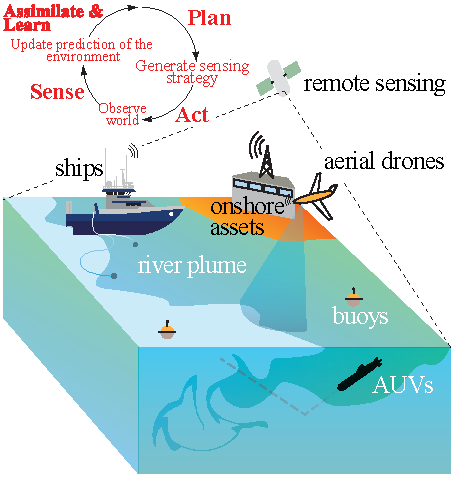
\includegraphics[width =
    0.49\textwidth]{Figures/envir2.pdf}\label{fig:envir1}}
  \hfill
  \subfigure[Frontal patterns off of the Nidelva river, Trondheim, Norway.]{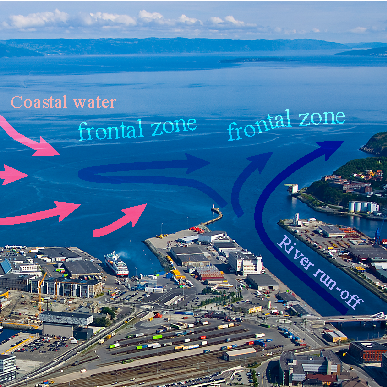
\includegraphics[width =
    0.49\textwidth]{Figures/river_proccess.pdf}\label{fig:nidelven}}
  \caption{\ref{fig:envir1} Traditional ocean observation based on
    ship-based sampling has recently been augmented by autonomous robotic vehicles. % and their interactions. 
    AUV platforms are an integral part of this network being able to reason and make decisions for efficient onboard adaptive sampling. % using the sense-plan-act control approach to autonomous control.
    \ref{fig:nidelven} The interaction of river and ocean creates
    processes that are challenging to map, where the combination of
    statistics and robotics can play a vital role in enabling more
    effective observation practices.}
\label{fig:envir}
\end{figure}

The AUVs considered here
operate at $1$-$3$ m/s in the upper water column. The in-water operation time capacity depends on survey speed, payload sensors and navigation. AUVs have limited computational capacity, and they are usually done on a single-board computer (SBC), like the Raspberry Pi or an multicore GPU NVIDIA Jetson TX1. 

%By deploying AUVs together with other resources, one can augment information from synthetic ocean models, remote-sensing data, or fixed-location sensors on buoys. 
Surveys with AUVs are usually limited to observations
along fixed transects that are pre-programmed by the human operator. This occurs on a spatial grid, called a waypoint graph. A more effective approach is to instead use onboard algorithms to continuously evaluate, update, and refine future sampling locations (sense-plan-act cycle in Fig. \ref{fig:envir1}), making the information
gathering \emph{adaptive} \citep{das11b,fossum18b,fossuminformation}. In doing so, the space of sampling opportunities is still limited by the waypoint graph, but the AUV has flexibility to 
modify its path at each waypoint based on what has been measured onboard
\citep{py10,Rajan12,Rajan12b}.

The application that is of focus in this work is towards spatial characterization of a frontal system generated by river
plumes. Fig. \ref{fig:nidelven} shows the survey area (Nidelva, Norway) where cold freshwater enters
from the river, creating a strong gradient in both temperature and
salinity. Because of the local topography and the Coreolis force
%\citep{coriolis1835memoire} 
the cold fresh water tends to flow near
land to the east, %. Depending on the river discharge, tidal effects,
%wind, and temperature differences, this boundary often gets
%distorted. Initial knowledge about the location and evolution of these
but the locations of these features are highly uncertain, making deterministic planning challenging. 

%River plumes belong to a class of ocean processes that are local and
%act on smaller \emph{sub-mesoscale} extent (from $5 m^2$ -- $10 km^2$) where
%lateral spatial variability tends to dominate. 
%At larger \emph{mesoscale} ($>50 km^2$), both three-dimensional space and time
%dynamics are important and can shift substantially, while in the case
%At this scale of river plumes one can further often limit scope to covering only lateral near surface spatial elements, and the case appears very amenable for AUVs usage. 
%However, the methodological framework can be extended to higher dimensional situations in a similar manner.

%\begin{figure}[!h] 
%\centering 
%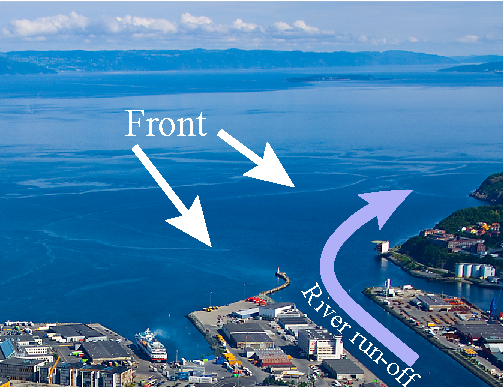
\includegraphics[width=0.85\textwidth]{Figures/pictures/c-updated.pdf}
%\caption{Frontal patterns off of the Nidelva river, Trondheim, Norway.}
%\label{fig:nidelven}
%\end{figure}

%\begin{figure}[!h]
%\centering
 % \subfigure[River front - Columbia River, Astoria, Oregon, US.]{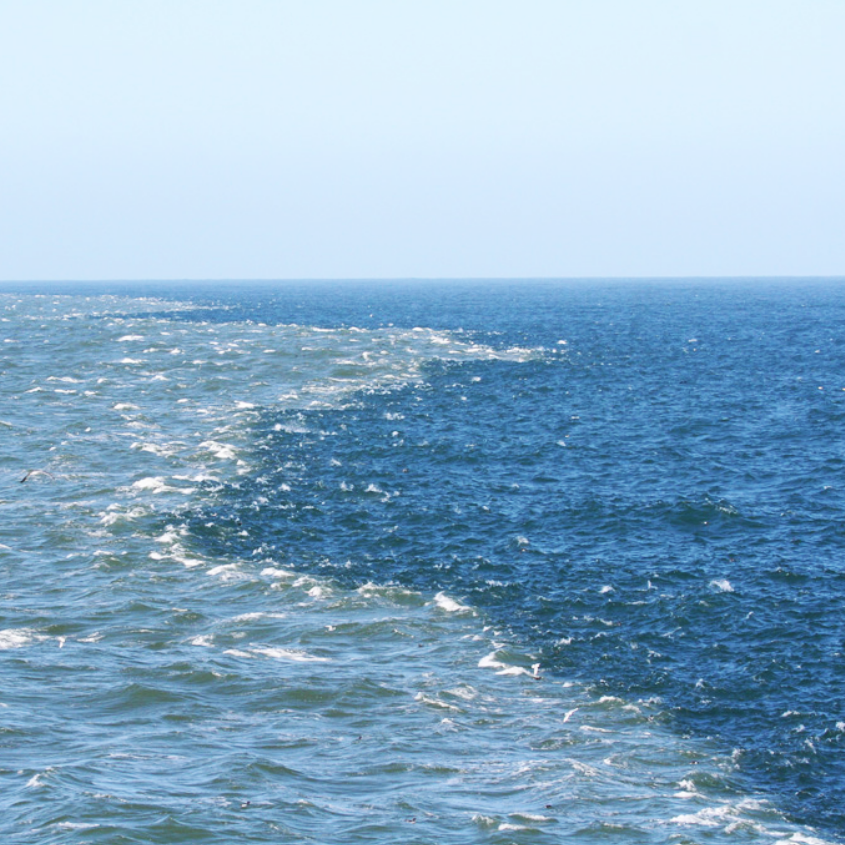
\includegraphics[width = 0.45\textwidth]{Figures/pictures/a.png}\label{fig:river1}}
 % \hfill
 %\subfigure[Tidal front - Korsfjorden, Norway.]{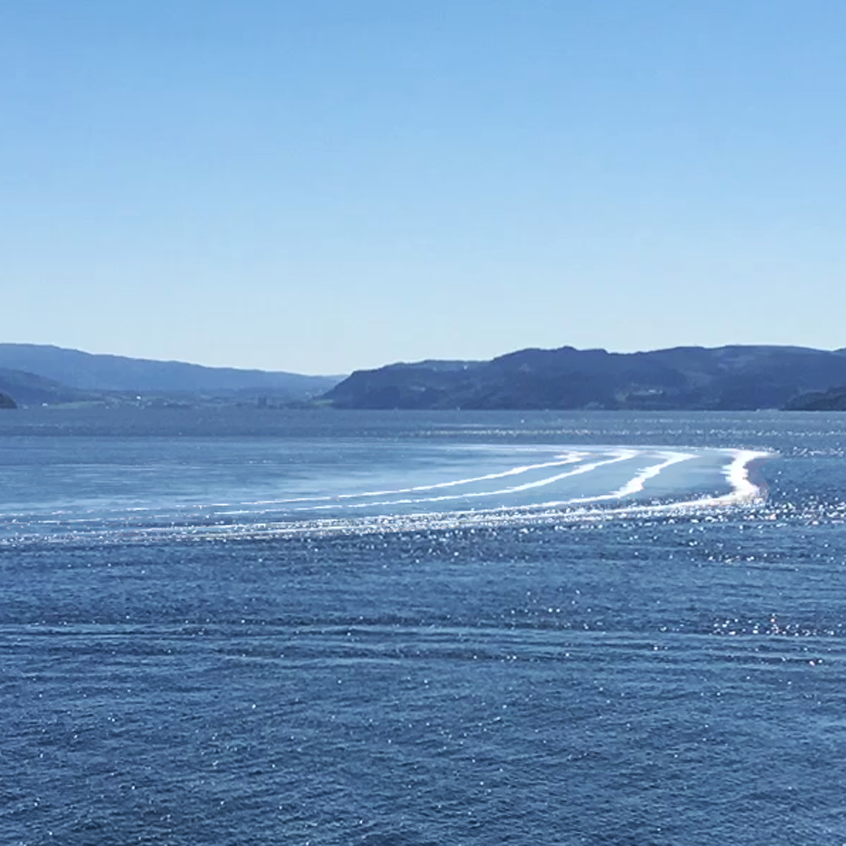
\includegraphics[width = 0.45\textwidth]{Figures/pictures/d.png}\label{fig:river2}}
 % \hfill
 % \subfigure[River plume - Rio de la Plata, Buenos Aires, Argentina.]{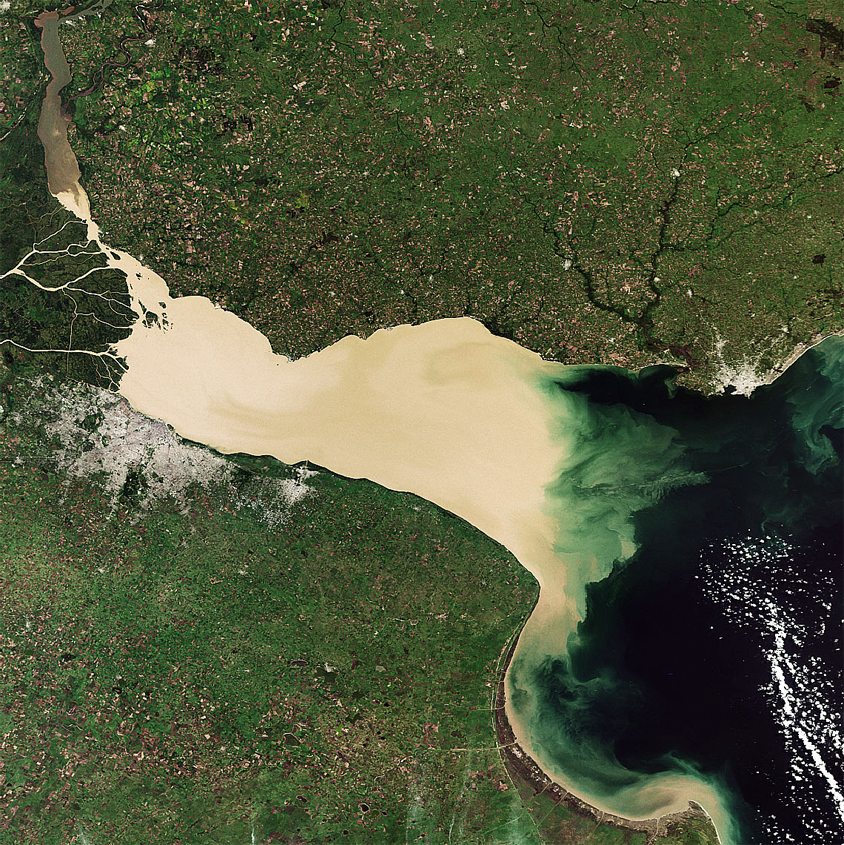
\includegraphics[width = 0.45\textwidth]{Figures/pictures/b.png}\label{fig:river3}}
 % \hfill
 %\subfigure[Frontal patterns - Nidelven, Trondheim, Norway.]{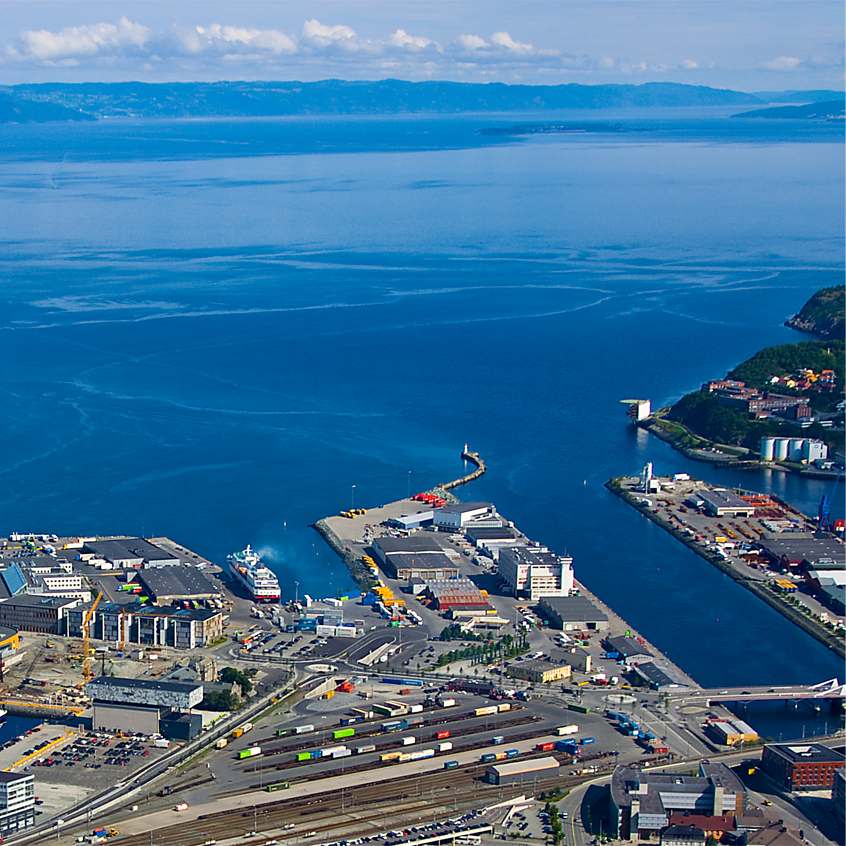
\includegraphics[width = 0.45\textwidth]{Figures/pictures/c.png}\label{fig:river4}}
 %\caption{Two examples of frontal features associated with
%   river-ocean interaction. % (\ref{fig:river1}) The river plume front of
   % the Columbia River meeting the Pacific Ocean.
%   (\ref{fig:river2})  Superimposed images (over 10 minutes) of a surface tidal front in
%   Korsfjorden, Norway. % (\ref{fig:river3}) The river plume of the Rio de
   % la Plata, taken by European Space Agency (ESA)'s Envisat platform and
   % MEdium Resolution Imaging Spectrometer (MERIS) sensor.
%   (\ref{fig:river4}) Aerial image of the mouth of the Nidelva river in
%   Trondheim, Norway where fresh water meets the salty fjord and creates
%   frontal patterns.} % Image courtesy: (\ref{fig:river1})
   % \cite{zamon2014marine}, (\ref{fig:river3}) ESA, CC BY-SA 3.0 IGO.}
% \label{fig:river_fronts}
%\end{figure}

%The use of \emph{robotic sampling} is motivated by the fundamental challenges of ocean observation, where a limited set of resources, a highly dynamic ocean, and the associated 

%This challenge can be addressed by employing more elaborate and adaptive sampling strategies that can capitalize on both prior and current observations in order to locate and map these areas.  



%\subsection{Autonomous Vehicles}


%To improve the state of sampling, modern tools and methods, including the use of autonomous platforms, oceanographic models and satellite remote sensing, needs to be combined with traditional data acquired by surface vessels or buoys (See Fig. \ref{fig:envir}). However, without adequate understanding of the theoretical underpinnings of how, when, and where to gather data, these tools and methods are insufficient in the vast and harsh oceans.

% retaining an advantageous strategy for information recovery, online during execution.
%The pressure on marine resources is growing and increased accuracy, resolution, and persistent monitoring of the oceans is crucial for long-term sustainable management. The impact of this research provides cost effective tools, techniques, and processes for doing ocean based measurements using robotic platforms. 
%adaptive design of experiments using robotic assets identifying and prioritizing relevant sampling locations on an information-theoretic basis. Spatial statistics naturally enters here through the ability to both model spatially correlated parameters and provide formal measures of uncertainty, on which this basis can be formed. 
%for oceanic sensing applications, where sensors are sparsely distributed and capitalizing on all available information is 

%This imperfect understanding of causality coupled with uncertainty implies that we need to obtain more measurements and use statistical models and methods to determine what and how phenomena form, to increase the quality of predictive statements. To improve the state of sampling, modern tools and methods, including the use of autonomous platforms, oceanographic models and satellite remote sensing, augment the more traditional data acquired by surface vessels or buoys (See Fig. \ref{fig:envir}). However, without adequate understanding of the theoretical underpinnings of how, when, and where to gather data, these tools and methods are insufficient in the vast and harsh oceans.

%There are several oceanographic data sources that can be used together with statistical tools to improve data collection in ocean science. In the following section we briefly discuss buoy data, satellite data, ocean models data, and AUV data.

%Buoy data provide very accurate information of oceanographic variables, but in most situations they are local, giving information only at one (north, east) coordinate, possibly with opportunities for conducting measurements at different depths. Gliders and other surface vessels are a kind of floating buoys that drift and can measure variables at many locations, but still with limited spatial coverage. 

%Satellite data are important for the mapping of oceanographic variables. They can also be indicative of variables such as temperature and salinity which we look at here, especially if the data are calibrated to for instance buoy data from the same spatial domain. However, the resolution of satellite data is relatively large, say $1 \times 1$ km $^2$ grid cells, and it only provides accurate information at the sea surface. Moreover, one cannot get useful satellite information on a cloudy day. 

%What is often done in practice is to run ocean models based on the complex differential equations governing oceanographic phenomena, where also satellite data can be assimilated and used as input, and possibly playing with different forcing mechanisms to capture some of the uncertainty of the models. Initial conditions, and can be used t the goal is to guide the sampling towards regions these regions, where we can reduce the uncertainty in the ES. These models provide insight that can be understood from practitioners, but they tend to be biased, and must also be calibrated to buoy data in one way or the other.

%to provide an effective specification of regions of phenomenological interest resolving the boundaries and the position of phenomena, on which evaluation of future sampling can be constructed.

%; some of these phenomena are illustrated in Fig. \ref{fig:envir2}. Figure \ref{fig:river_fronts} illustrates the %phenomena of interest in this paper, which is river plumes and their interaction with the ocean.

%Feature driven sampling
%processes acting across a wide range of spatio-temporal scales makes prioritizing sampling efforts necessary. %Autonomous robotic platforms, can address these issues by providing the ability to focus sampling efforts to %high-interest regions (``hotspots").


% Determining paths for mobile robotic sensors in order to maximize the
% information gained about an environment is formally known as informative
% path planning. This, and related problems such as the orienteering
% problem \citep{Golden87}, has been studied in the context of graphs,
% where the potential measurement are assigned to nodes on which
% evaluation of different routes can be conducted.
%In this context, a fundamental result from \cite{nemhauser1978analysis} proves that a simple greedy algorithm (iteratively selecting the location which most increases the utility) can achieve a near-optimal solution if the problem can be shown to be \emph{submodular}\footnote{an intuitive diminishing returns property, where the informative value of adding sensors decrease with the number of sensors added.}. Building on this result, \cite{chekuri2005recursive} explored this in the setting of a graph using a recursive greedy algorithm, providing near-optimal solutions depending on the planning horizon and graph resolution. 

Adaptive in-situ AUV sampling of an evolving frontal feature has been explored in
\cite{fronts11,Zhang2012,Pinto2018,costa19}. These approaches
typically use a reactive-adaptive scheme, whereby exploration does not
rely on a statistical model of the environment, but rather adapts
based on closing the sensing and actuation loop. Myopic sampling, i.e. stage-wise selection of
the path (on the waypoint graph), has been used for surveys
\citep{singh2009efficient,Binney2013} that focus largely on reducing
predictive variance or entropy. These criteria are widely adopted in the statistics literature on spatio-temporal design as well \cite{bueso1998state,zidek2019monitoring}, but variance and
entropy reduction are independent of the actual data realizations
under the assumptions of GP models, so limited decision flexibility is created for sequential designs. The use of data-driven adaptive
criteria was introduced to include more targeted sampling of regions
of scientific interest in \cite{Low2009} and \cite{fossuminformation}.
In this paper, with a focus on mapping the river plume by rewarding the
designs that improve the classification of ES in temperature and salinity.

%\begin{figure}[h]
%\centering
%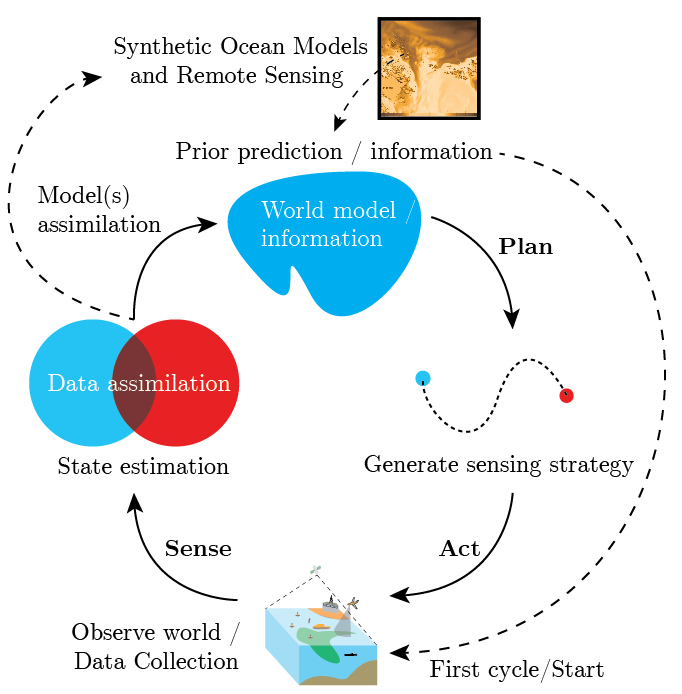
\includegraphics[width=0.4\textwidth]{Data-driven.png}
%\label{fig:auv_alone}
%\caption{The concept of data-driven sampling.}
%\end{figure}

%The goal is effectively map the extension of the river plume given this


%, we can formulate this question as follows: the ocean region  defined by the boundary between water bodies, separated by a characteristic temperature gradient that is smaller than $T=5$\textdegree C and a salinity concentration lower than $S=30$ [g/kg]. A goal is then to improve our predictive capabilities to answer this question better.
%For example,  (examples are shown in Fig. \ref{fig:river_fronts}). However, 

% In doing so, the aim is to increase the knowledge about the uncertain ocean environment through adaptive sampling

\section{Excursion Sets and Integrated Bernoulli Variance}
\label{sec:ESEP}

\cite{adler2000excursion,adler2009random}.

Our objective is to leverage statistical tools to characterize a river
plume, focusing on spatial separation of cold freshwater from the
river and warmer saline waters of the fjord. ES and EPs are useful
starting points to measure the ability to classify water masses. The
goal of experimental sampling is to improve this
characterization, as quantified via changes in the EPs.

We consider a lateral domain near the sea surface, with locations
$\bx \in \mathcal{M} \subset \mathbf{R^2}$. The two variables of
interest, temperature and salinity, are defined as random processes:
$\xi_T(\bx)$ denotes the temperature (in $^o C$) and $\xi_S(\bx)$
denotes the salinity (in $g/kg$) at location $\bx$. The generalization
to more than two variables is given in Section \ref{gen_k}, and the
adaptive sampling strategies are described in Section
\ref{sec:heuristics}.

We let $t_T$ be a threshold for temperature and $t_S$ a threshold for
salinity. The joint ES is then defined by:
\begin{equation}\label{ES}
     \mbox{ES} = \{\bx \in \mathcal{M} | \xi_T(\bx) \leq t_T,\xi_S(\bx) \leq t_S\}.
\end{equation}
The excursions could also be defined as larger than a threshold, or
within a boundary of limits for the two variables; calculations and
interpretations will be similar in these cases.

The ES holds random indicator variables while the associated EPs are: 
\begin{equation}\label{eq:prob}
  p(\bx) = P(\xi_T(\bx) \leq t_T, \xi_S(\bx) \leq t_S), \hspace{3mm} \bx \in \mathcal{M}.
\end{equation}
If the EPs in Eq. (\ref{eq:prob}) are
close to $1$ or $0$ at a given location, it is easy to classify water mass at this point as either river or ocean; it is, however,
challenging if the probability is close to $0.5$. 
The IBV, see \cite{bect2019}, is defined as:
\begin{equation}\label{measVAR}
    V = \int_{\bx \in \mathcal{M}} p(\bx) \left(1-p(\bx)\right) d\bx.
\end{equation}

Data can be
gathered at selected locations of the domain $\mathcal{M}$, to improve
classification performance. We denote temperature measurements by
$y_{T}(\bx_i)$ and salinity measurements by $y_{S}(\bx_i)$ at a
sampling location $\bx_i \in \mathcal{M}$. Given a set of
measurements denoted $\by$, the conditional EPs are:
\begin{equation}\label{eq:post_ep}
 p(\bx;\by) = P(\xi_T(\bx) \leq t_T, \xi_S(\bx) \leq t_S |\by). 
\end{equation}

Our goal is to construct adaptive sampling strategies based on
continuous evaluation of the EPs. As the EPs provide a description of
the boundary uncertainty, the strategies can effectively use this
description to prioritize sampling efforts at locations that are
ambiguous, making exploration more effective. It is natural to
evaluate the expected reduction in the IBV, conditioned on the survey
data. The expected updated IBV is:

\begin{equation}\label{sur}
    V_{\mbox{upd}} = \int_{\bx \in \mathcal{M}} E_{\by} \left( p(\bx;\by)\left( 1-p(\bx;\by)\right) \right) d\bx, 
\end{equation}
where the expectation is over the planned data, and the probability is
defined in Eq. (\ref{eq:post_ep}).  Considering a set $\mathcal{J}$ of
possible designs for an AUV survey, a criterion for the selection is:
\begin{equation}\label{crit}
    j^* = \mbox{argmin}_{j \in \mathcal{J}} V_{\mbox{upd}}(j),
\end{equation}
where the criterion $V_{\mbox{upd}}(j)$ in Eq. (\ref{sur}) is computed
for each of the possible designs. 

%Recent work on ESs and EPs connected to spatial statistics include
\cite{picheny2010,french2013spatio,bolin2015excursion,french2016credible}.
%Our focus is on ES as defined in Eq. (\ref{ES}) and the uncertainty
%reduction achieved by sampling as in Eq. (\ref{sur}). In this sense,
%our work is similar to \cite{bect2012}, \cite{chevalier2014fast}, and
%\cite{azzimonti2016quantifying} who describe analytical results for
%the IBV for univariate processes. A major contribution of our work is
%to derive closed-form results for this design criteria for situations
%where the underlying model is based on multivariate GPs.

\section{Gaussian Processes and Excursion Probabilities}
\label{sec:GP_EP}

Calculations of the EPs and the IBV require a model specification. We
use GP models, which provide a practical and popular probabilistic
approach to modeling environmental data, and allows a closed form
evaluation of the IBVs as derived in Section \ref{sec:sur}. GPs can
also be fitted to run onboard robotic vehicles with limited
computational assets, such as AUVs.

\subsection{Bivariate GPs}

The Gaussian model is used to represent the bivariate random fields of
temperature and salinity. At location $\bx \in \mathcal{M}$, the
bivariate distribution is:
\begin{equation}\label{gp_bar}
  \begin{bmatrix}\xi_T(\bx) \\
    \xi_S(\bx) \end{bmatrix}
 \sim N \left( 
\begin{bmatrix} \mu_{T}(\bx)\\
\mu_{S}(\bx)
\end{bmatrix},\begin{bmatrix}
\sigma_{T}^2(\bx) & \sigma_{T}(\bx) \sigma_S(\bx) \gamma(\bx)  \\
\sigma_{T}(\bx) \sigma_S(\bx) \gamma(\bx)  & \sigma_{S}^2(\bx) 
\end{bmatrix}
\right),
\end{equation}
where the notation refers to Gaussian (i.e. normal) distributed
variables specified by the mean vector and covariance matrix. For the
application of a river plume, the model parameters are specified from
a short preliminary survey. The means vary with location, capturing
the variability near the river mouth, while the variance parameters
and correlation between salinity and temperature are assumed to be
constant for all locations. %and within each water mass.

For the spatial dependence among variables, we assume a separable
correlation function with the same decay for salinity and temperature,
which is consistent with expectations for a river plume where the
decay is related to common water masses (Section
\ref{sec:case_study}). In the resulting function, we have:
\begin{equation}\label{gp_corr}
\mbox{Cov}(\xi_i(\bx),\xi_j(\bx')) = \rho(\bx,\bx') \sigma_i \sigma_j (\gamma +(1-\gamma )\delta_{ij}), \\
\end{equation}
where for $i,j \in {T,S}$ and $\delta_{ij}=1$ if $i=j$, and
$\delta_{ij}=0$ otherwise. Moreover, we assume stationary isotropic
random fields where the correlation function $\rho(\bx,\bx')$
solely depends on $\bx$ and $\bx'$ via Euclidean distance
$h=\sqrt{||\bx-\bx'||^2}$. With data and prior knowledge, one could
possibly fit and estimate parameters of non-stationary or
non-isotropic covariance functions and more complex multivariate
spatial covariance functions
\citep{gneiting2010matern,genton2015cross}; however, that is left for
future work.

We discretize the spatial domain $\mathcal{M}$ to a set of $n$ grid
locations $\mathcal{M}_g = \{\bx_i, i=1,\ldots,n \}$, where each cell
has area $\Delta$; the grid is used for the waypoint graph setting the
possible design locations. It is also used when solving integral
expressions in Eq. (\ref{measVAR}) and (\ref{sur}), which are then
approximated by sums over all grid cells. Using vector notation, we
denote the Gaussian temperature and salinity variables on the grid and
its density function by the formula:
\begin{equation}\label{prior}
    \bxi = (\xi_T(\bx_1),\xi_S(\bx_1),\ldots,\xi_T(\bx_n),\xi_S(\bx_n))^t, \hspace{3mm}
    \bxi  \sim  N(\bmu, \bSigma). %\pi (\bxi) & =& \frac{1}{(2\pi)^{n}|\bSigma|^{\frac{1}{2}}}e^{-\frac{1}{2}(\bxi -\bmu)^T\bSigma^{-1}(\bxi-\bmu)}.
\end{equation}
%Here, $\pi(\bxi)$ is the joint density function of length $2 n$ vector $\bxi$, and
The length $2n$ vector $\bmu$ contains the expected values of
temperature and salinity at the grid locations, while the
$2n \times 2n$ matrix $\bSigma$ contains the
variance-covariances of temperature and salinity variables at all grid
locations.

\subsection{Data Model and Updating of GPs}

Data are gathered by an AUV that can measure temperature and salinity
at a subset of locations on the defined grid. This can be done in a
static manner (where the survey design is pre-planned), or in a
sequential way with several stages of data gathering. For the latter,
a stage of data is gathered first, and then assimilated to get an
updated model. Then the updated model is used to design and select the
next stage of measurements, and so on (Section
\ref{sec:heuristics}). Below, we describe the model for one stage of
data and the Gaussian formula for a single update.

We denote the data at $n_y$ locations by
$\by=(y_{T,1},y_{S,1},\ldots,y_{T,n_y},y_{S,n_y})^t$, representing the
temperature and salinity measurements gathered at the first stage of
nodes in the grid. The conditional model for the data, given the true temperature
and salinity, is described by: 
\begin{equation}\label{likelihood}
\by | \bxi \sim N( \bG \bxi, \bR), %\pi(\by | \bxi)= \frac{1}{(2\pi)^{m}|\bR|^{\frac{1}{2}}}e^{-\frac{1}{2}(\by -\bG\bxi)^T\bR^{-1}(\by-\bG\bxi)},
\end{equation}
where $\bG$ is a $2n_y \times 2n$ matrix containing '$1$'s on the
measurement indices of the grid and '$0$' otherwise. The size
$2n_y \times 2n_y$ covariance matrix $\bR$ contains zeroes except on the diagonal entries, which are set to $r^2_T$ and $r^2_S$, holding the measurement error variances of temperature and salinity observations.

The GP mean and covariance in Eq. (\ref{prior}) are updated in the
model when more information is available. The updated distribution for
temperature and salinity variables on the spatial grid, given survey
data $\by$, is Gaussian with mean and covariance:
\begin{eqnarray}\label{gp_upd}
  \bm &=& \bm(\by) = \bmu+\bSigma \bG^t (\bG \Sigma \bG^t+\bR)^{-1}(\by-\bG \bmu),  \\
  \bA &=& \bSigma - \bSigma \bG^t (\bG \bSigma \bG^t+\bR)^{-1} \bG
          \bSigma.\nonumber
\end{eqnarray}

The updated bivariate distribution at a grid location $\bx \in
\mathcal{M}_g$ is then: 
\begin{equation}\label{gp_hat}
\begin{bmatrix}
\xi_T(\bx) \\
\xi_S(\bx)
\end{bmatrix}
 |\by
 \sim N \left( 
\begin{bmatrix} m_{T}(\bx)\\
m_{S}(\bx)
\end{bmatrix},\begin{bmatrix}
a_{T}^2(\bx) & a_{T,S}(\bx)  \\
a_{T,S}(\bx)  & a_{S}^2(\bx)  
\end{bmatrix}
\right),
\end{equation}
with entries extracted from the conditional mean and covariance
expressions in Eq. (\ref{gp_upd}).

% The conditional mean $\bm$ will be important in the following
% derivation in Section \ref{sec:sur}.
The calculation of the design criterion in Eq. (\ref{sur}) requires
the marginal distribution of the data which is defined over $\bxi$ to
be $\by \sim N( \bG \bmu,\bG \bSigma \bG^t+\bR)$.  However, it turns
out that a simplified form of the calculation is possible because the
conditional mean in Eq. (\ref{gp_hat}) is a linear (affine) function of
the data $\by$ and the covariance is not a function of the data.
Before inputting the data, the distribution of the conditional mean is:
\begin{equation}\label{distxi} \bm \sim N(\bmu , \bPsi), \hspace{3mm}
  \bPsi=\bSigma \bG^t (\bG \bSigma \bG^t+\bR)^{-1} \bG \bSigma.
\end{equation} 
When considering only grid location $\bx$, we can
extract elements from its mean vector and covariance matrix to get the
bivariate distribution:
\begin{equation}\label{dist_mxi}
  \bm(\bx) \sim N \left( \begin{bmatrix}
      \mu_{T}(\bx) \\
      \mu_{S}(\bx) \end{bmatrix}, \begin{bmatrix}
      \psi^2_{T}(\bx) & \psi_{T,S}(\bx)\\
      \psi_{T,S}(\bx) & \psi^2_{S}(\bx) \end{bmatrix} \right),
\end{equation}
which is important for the derivation of the closed-form solution of the design criteria.

\section{Uncertainty reduction in excursion sets}
\label{sec:sur}

\subsection{EPs for GPs}

Based on Gaussian modeling assumptions, the EPs can be computed at any
location $\bx$. Without additional data, Eq.  (\ref{eq:prob}) gives:
\begin{eqnarray}\label{eq:prob_mv0}
 p(\bx) &=& P(\xi_T(\bx) \leq t_T, \xi_S(\bx) \leq t_S) \nonumber \\
 &=& \Phi_2 \begin{pmatrix} 
\begin{bmatrix} t_T\\
t_S
\end{bmatrix};
\begin{bmatrix} \mu_{T}(\bx)\\
\mu_{S}(\bx)
\end{bmatrix},\begin{bmatrix}
\sigma_{T}^2(\bx) & \sigma_{T}(\bx)\sigma_{S}(\bx) \gamma(\bx)  \\
\sigma_{T}(\bx)\sigma_{S}(\bx) \gamma(\bx)  & \sigma_{S}^2(\bx)  
\end{bmatrix}\end{pmatrix},
\end{eqnarray}
where $\Phi_2$ is the bivariate Gaussian cumulative distribution
function, and the mean and covariance entries are as defined in
Eq. (\ref{gp_bar}).

When data $\by$ are available, Eq. (\ref{eq:post_ep}) similarly gives:
\begin{eqnarray}\label{eq:prob_mv}
 p(\bx;\by) &=& P(\xi_T(\bx) \leq t_T, \xi_S(\bx) \leq t_S |\by)
 \nonumber \\
 &=& \Phi_2 \begin{pmatrix} 
\begin{bmatrix} t_T\\
t_S
\end{bmatrix};
\begin{bmatrix} m_{T}(\bx)\\
m_{S}(\bx)
\end{bmatrix},\begin{bmatrix}
a_{T}^2(\bx) & a_{T,S}(\bx)  \\
a_{T,S}(\bx)  & a_{S}^2(\bx)  
\end{bmatrix}\end{pmatrix},
\end{eqnarray}
with parameters as defined in Eq. (\ref{gp_upd}) and
(\ref{gp_hat}). Here, the probabilities would not only depend on the
data but also on the data design defined via matrix $\bG$ in
Eq. (\ref{likelihood}). We next derive results that simplify the
comparison of several designs.

\subsection{Expected IBV for Bivariate Models}

We will next derive closed-form solutions for the expectation in
Eq. (\ref{sur}). The location index $\bx$ is suppressed to avoid
overly complex notation. We present new results for computing the
expectation in the integral of Eq. (\ref{sur}).

A critical first element in the derivation is using the GP model and the
linear dependence on $\by$ in the conditional mean in
Eq. (\ref{gp_upd}). This results in a closed form Gaussian
distribution for the conditional mean in Eq. (\ref{dist_mxi}). The
high-dimensional inner integral in Eq. (\ref{sur}) then reduces to a
bivariate integral \citep{bhattacharjya2013value, chevalier2014fast},
with an expectation over $\bm=(m_{T},m_{S})^t$.  We standardize the two
variables in Eq. (\ref{sur}) as   $Z_T=\frac{\xi_T-m_{T}}{a_{T}}$,
$Z_S=\frac{\xi_S-m_{S}}{a_{S}}$, with
$\mbox{Corr}(Z_T,Z_S)=a_{T,S}/(a_{T} a_{S})=\eta_{T,S}$, and we can
then rephrase the probability as: 
\begin{eqnarray}\label{ytom}
   P(\xi_T \leq t_T, \xi_S \leq t_S|\by) &=& P \left( Z_T \leq\frac{t_T-m_{T}}{a_{T}}, Z_S \leq\frac{t_S-m_{S}}{a_{S}}|\by \right) \nonumber \\
   &=& \Phi_2 \begin{pmatrix} 
\begin{bmatrix} \frac{t_T-m_{T}}{a_{T}}\\
\frac{t_S-m_{S}}{a_{S}}
\end{bmatrix};
 \begin{bmatrix} 0\\
0
\end{bmatrix},\begin{bmatrix}
1 & \eta_{s,t}  \\
\eta_{s,t}   & 1  
\end{bmatrix}\end{pmatrix} \nonumber \\
&=& P(\xi_T \leq t_T, \xi_S \leq t_S|\bm).
\end{eqnarray}
Since the expression only depends on $\by$ via its affine function
$\bm$, the expectation in Eq. (\ref{sur}) is reduced to a bivariate
integral over $\bm$.  Introducing $\pi(\bm)$ for the density function
of $\bm$, the expected Bernoulli variance becomes:
\begin{eqnarray}
\label{eq:var2}
E_{\by}(p(1-p)) &=& E_{\bm}(p(1-p)), \hspace{3mm} p=P(\xi_T \leq t_T, \xi_S \leq t_S|\bm) \nonumber \\
E_{\bm}(p(1-p)) & = & \int p(1-p) \pi(\bm) d\bm, \nonumber \\
 &=& \int P(\xi_T \leq t_T, \xi_S \leq t_S|\bm)  \pi(\bm) d\bm \nonumber  \\
&-& \int P(\xi_T \leq t_T, \xi_S \leq t_S|\bm) P(\xi_T \leq t_T, \xi_S \leq t_S|\bm) \pi(\bm) d\bm. 
\end{eqnarray}
We will next extend results of \cite{chevalier2014fast} to solve for
these two parts (see also \cite{stroh}).

For the first part of the integral above, we have:
\begin{equation}
\label{part1:phi2}
 \int P(\xi_T \leq t_T, \xi_S \leq t_S|\bm) \pi(\bm) d\bm= 
P \left( Z_{T} \leq \frac{t_T-m_{T}}{a_{T}}, 
Z_{S} \leq \frac{t_S-m_{S}}{a_{S}} \right). \nonumber
\end{equation}
The standardized variable $\bZ=(Z_{T},Z_{S})$ is chosen to be independent of $\bm$. Using Eq. (\ref{dist_mxi}), we have:
\begin{equation}
    E(a_{T} Z_{T}+m_{T}-t_T) = \mu_{T}-t_T, \hspace{3mm}
    \mbox{Var}(a_{T} Z_{T}+m_{T}-t_T) = a^2_T+ \psi^2_{T} 
\end{equation}
for the temperature part; the same holds for salinity. From this we
get:
\begin{eqnarray}\label{two_parts0}
& P & \left( Z_{T} \leq \frac{t_T-m_{T}}{a_{T}}, 
Z_{S} \leq \frac{t_S-m_{S}}{a_{S}} \right) \\
&=& \Phi_2 \begin{pmatrix} 
\begin{bmatrix} 0\\
0
\end{bmatrix};
\begin{bmatrix} \mu_{T}-t_T\\
\mu_{S}-t_S
\end{bmatrix},\begin{bmatrix}
a^2_T+ \psi^2_{T} & a_{T,S}+\psi_{T,S}  \\
a_{T,S}+\psi_{T,S}   & a^2_T+ \psi^2_{T} 
\end{bmatrix}\end{pmatrix} \nonumber.
\end{eqnarray}

For the second part of the expression Eq.(\ref{eq:var2}), standardization
implies that: 
\begin{eqnarray}\label{part1:phi4}
&& \hspace{6mm} \int P(\xi_T \leq t_T, \xi_S \leq t_S|\bm) P(\xi_T \leq t_T, \xi_S \leq t_S|\bm) p(\bm) d\bm =  \\
&P& \hspace{-3mm} \left( Z_{1,T} \leq \frac{t_T-m_{T}}{a_{T}}, 
Z_{1,S} \leq \frac{t_S-m_{S}}{a_{S}},Z_{2,S} \leq \frac{t_T-m_{T}}{a_{T}}, 
Z_{2,S} \leq \frac{t_S-m_{S}}{a_{S}} \right). \nonumber
\end{eqnarray}
Here, $\bZ_1=(Z_{1,T},Z_{1,S})$, $\bZ_2=(Z_{2,T},Z_{2,S})$ are
independent bivariate zero-mean and unit-variance Gaussian vectors,
both with element-wise correlation $\eta_{T,S}$. Moreover, $\bZ_1$ and
$\bZ_2$ are chosen to be independent of $\bm$, hence:

\begin{equation}
\small
\label{eq:22}
    \left(
    \begin{array}{cccccc}
         Z_{1,T} \\
         Z_{1,S} \\
         Z_{2,T} \\
         Z_{2,S} \\
         m_{T} \\
         m_{S}
    \end{array}
    \right)
\sim N \left(
\left(
    \begin{array}{cccccc}
    0 \\
    0 \\
    0 \\
    0 \\
          \mu_{T} \\
         \mu_{S} 
    \end{array}
    \right),
   \left[ 
      \begin{array}{cccccc}
        1 & \eta_{T,S} & 0 & 0 & 0 & 0  \\
        \eta_{T,S} & 1 & 0 & 0 & 0 & 0 \\
        0 & 0 & 1 & \eta_{T,S} & 0 & 0 \\
        0 & 0 & \eta_{T,S} & 1 & 0 & 0 \\
        0 & 0 & 0 & 0 & \psi^2_{T} & \psi_{T,S} \\
        0 & 0 & 0 & 0 & \psi_{T,S} & \psi^2_{S} 
    \end{array}
\right]
\right).
\vspace{0.2cm}
\end{equation}

The solution to the second part of Eq. \eqref{eq:22} can be found by
evaluating a four-variable cumulative distribution function associated
with Eq. (\ref{part1:phi4}), accounting for the mean, variance and
covariances of $\bZ_1$, $\bZ_2$ and $\bm$ in the appropriate linear
combinations. Using vector-matrix formulations, we define the linear
combinations:
\begin{equation}
\label{Vcomb}
    \bV=\left[
    \begin{array}{cccccc}
        a_T & 0 & 0 & 0 & 1 & 0 \\
         0 & a_S & 0 & 0 & 0 & 1 \\
         0 & 0 & a_T & 0 & 1 & 0\\
         0 & 0 & 0 & a_S & 0 & 1\\
    \end{array}
    \right] 
    \left(
    \begin{array}{cccccc}
         Z_{1,T} \\
         Z_{1,S} \\
         Z_{2,T} \\
         Z_{2,S} \\
         m_{T} \\
         m_{S}
    \end{array}
    \right),
\end{equation}
which in turn then becomes:
{\small
\begin{eqnarray}
\label{part1:phi4_2}
&&P \left( Z_{1,T} \leq \frac{t_T-m_{T}}{a_{T}}, 
Z_{1,S} \leq \frac{t_S-m_{S}}{a_{S}}, Z_{2,S} \leq \frac{t_T-m_{T}}{a_{T}}, Z_{2,S} \leq \frac{t_S-m_{S}}{a_{S}} \right)\\
&=&  \Phi_4 
\begin{pmatrix} 
\begin{bmatrix} t_T\\
t_S \\
t_T \\
t_S
\end{bmatrix};
E( \bV),Var(\bV)
\end{pmatrix} \nonumber.
\end{eqnarray}
}
The multivariate cumulative probabilities in two and four dimensions
are computationally efficient using methods developed by
\cite{genz2009computation}.  In the end, the first part in
Eq. (\ref{two_parts0}) and the second in Eq. (\ref{part1:phi4}) are
computed for each location on the grid and summed over
$\bx \in \mathcal{M}_g$, to get the design evaluation criterion in
Eq. (\ref{sur}).

\subsection{Generalization to the Multivariate Case}
\label{gen_k}

In our application domain with the variables temperature and salinity,
the solutions to the complex integral equations for the expected IBV
are reduced to calculating bivariate and four-variate cumulative
distribution functions for Gaussian vectors. For the more general
case, one would be interested in $K$ random fields. In the ocean
sciences, the variables could include chlorophyll or other
bio-geochemical quantities in addition to temperature and salinity.

The equations derived in the previous section can then be generalized. Let
$\bxi(\bx)=(\xi_1(\bx),\ldots,\xi_K(\bx))$, and the expected Bernoulli
variance is:
\begin{equation}\label{two_partsK}
E_{\by}(p(\bx;\by)(1-p(\bx;\by))), \hspace{3mm} p(\bx;\by)=P(\xi_k(\bx) \leq t_k ; k=1,\ldots,K|\by). 
\end{equation}
From the first key result of linear combination of Gaussian variables,
we reduce the integral to a $K$ dimensional integral of the relevant
$\bm=E(\bxi(\bx)|\by)$. Next, reducing the integral to two parts, we
standardize the variables and compute cumulative distributions.  In
summary, we get:
\begin{equation}\label{two_parts}
E_{\by}(p(\bx)(1-p(\bx))) =  \Phi_K 
\begin{pmatrix}
\begin{bmatrix} t_1\\
\vdots \\
t_K 
\end{bmatrix};
\bmu,\bA+\bPsi 
\end{pmatrix}
- \Phi_{2K} 
\begin{pmatrix}
\begin{bmatrix} t_1\\
\vdots \\
t_K \\
t_1\\
\vdots \\
t_K 
\end{bmatrix};
E(\bV),Var(\bV) 
\end{pmatrix},\nonumber
\end{equation}
where $\bA$ and $\bPsi$ are direct $K$-variate extensions of the
matrices in Eq. (\ref{two_parts0}), and the matrix $\bV$ finds the
relevant linear combination of two independent vectors
$\bZ_l=(Z_{l,1},\ldots,Z_{l,K})$, $l=1,2$ and $\bm$, as an extension
of Eq. (\ref{Vcomb}).

\subsection{An Example of IBV using Temperature and Salinity}

In this section, we calculate EPs and the Bernoulli variance for a few bivariate
Gaussian distributions to illustrate the concepts articulated above.
Fig. \ref{illus_bivarDens} shows contour plots of three different
densities with increasing correlation $\gamma$ between temperature and
salinity.
\begin{figure}[h!] \centering
  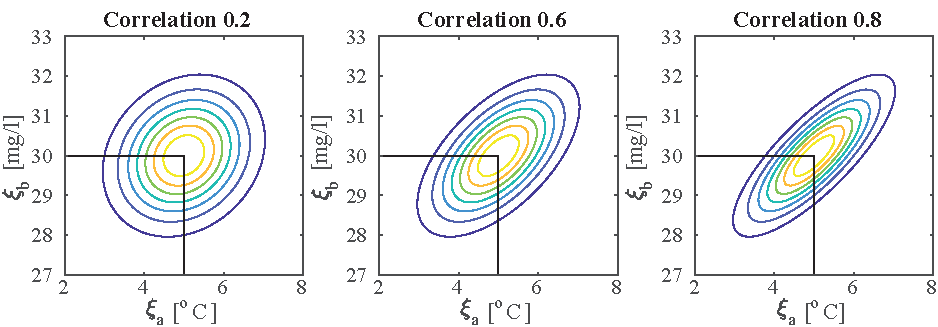
\includegraphics[width=0.99\textwidth]{Figures/illus_bivar.pdf}
  \caption{Density contour plots with different correlations between
    temperature and salinity. The densities have unit variance and the
    thresholds are identical to the mean values $5^o C$ and
    $30 mg/l$. X-axis is temperature and y-axis is salinity.}
\label{illus_bivarDens}
\end{figure}
Here, the thresholds are set equal to the mean $\mu_T=t_T=5^o C$, and
salinity $\mu_S=t_S=30$ mg/l. The displayed densities have unit
standard deviations for both temperature and salinity, but we also
study the effect of doubling the standard deviations.

Table \ref{tab:sim_rhoab} shows the initial EPs and the associated Bernoulli
variance (second row) for the examples indicated in
Fig. \ref{illus_bivarDens}. The EPs increase with the correlation as
there is a strong tendency to have concurrently low temperature and
salinity. The Bernoulli variance is similarly large for high
correlations. EPs and Bernoulli variances are the same for standard
deviation $1$ or $2$, which implies that high variability in
temperature and salinity is not captured in the $p(1-p)$ expression.

\begin{table}[!h] \centering \caption{EP and Bernoulli variance for
    different correlations and variances (top rows), and expected
    Bernoulli variances for both temperature and salinity data $\by$ and 
    temperature $y_T$ (bottom rows).}
  \begin{tabular}{c|ccc|ccc}
 &\multicolumn{3}{c}{$\sigma_S=\sigma_T=1$} & \multicolumn{3}{c}{$\sigma_S=\sigma_T=2$} \\
\hline
Correlation $\gamma$ & 0.2 & 0.6 & 0.8 & 0.2 & 0.6 & 0.8 \\
\hline
$p$ & 0.28 & 0.35 & 0.40 & 0.28 & 0.35 & 0.40 \\ 
$p(1-p)$ & 0.20 & 0.23 & 0.24 & 0.20 & 0.23 & 0.24 \\ 
$E_{\by}(p(\by) (1-p(\by)))$ & 0.092 & 0.089 & 0.085 & 0.052 & 0.051 & 0.049 \\ 
$E_{y_T}(p(y_T) (1-p(y_T)))$ & 0.151 & 0.138 & 0.123 & 0.137 & 0.114 & 0.093 \\ 
\hline
\end{tabular}
\label{tab:sim_rhoab}
\end{table}

Table \ref{tab:sim_rhoab} (bottom two rows) shows results of expected
Bernoulli variance calculations. This is presented for a design
gathering both data types $(y_T,y_S)$, and for a design with
temperature measurements $y_T$ alone. With both data,
$(y_T,y_S)^t=(\xi_T,\xi_S)^t+N(0,0.5^2\bI)$, while
$y_T=\xi_T+N(0,0.5^2)$ when only temperature is measured.  For this
illustration, Table \ref{tab:sim_rhoab} shows that the expected
Bernoulli variance gets lower with larger standard deviations
$\sigma_T$ and $\sigma_S$ (right columns). The reduction of Bernoulli
variance is largest for the cases with high correlation
$\gamma$. Albeit smaller, there is also uncertainty reduction when
only temperature is measured (bottom row), especially when temperature
and salinity are highly correlated. When correlation is low
($\gamma=0.2$), there is little information about salinity in the
temperature data, and therefore less uncertainty reduction. In an
application with fresh cold water from a river source, the temperature
and salinity variables will not only be interdependent, but will also
likely show dependence in the spatial dimension. This in turn will
impact the design criteria when we evaluate the information measure by
integrating over several locations (Section \ref{sec:case_study}).

%\subsection{Expected classification criteria}

%{\bf{I have not done anything here - skip this, I think}}.

%Rather than minimizing expected variance one can aim at minimizing the classification probability of the excursion set: 
%$\min [p,(1-p) ]$, see e.g. \cite{lilleborge2016information}. 

%Again, since the conditional mean is a linear in the data, we only have to look at the %relevant linear combination via $\bm_{\xi}=E(\bxi)$.
%See also \cite{bhattacharjya2013value}.

%\begin{equation}
%E(\min \{ p,(1-p)\})=\int \min P(\xi_T \leq t, \xi_S \leq s),[1-P(\xi_T \leq t, \xi_S \leq s)] p(E(\bxi)=) dE(\bxi)=,
%\end{equation}
%for the complementary probabilities, this is again evaluated by the corner regions for the block, and $\Phi_4()$ evaluations are required.

%In the end, this result is integrated over the spatial domain $x \in X$.

\section{Sequential updating and heuristic path planning}\label{sec:heuristics}

An important concept underlying this work is the potential of robotic
sampling to adapt survey plans based on data and statistical methods
in accordance with the sense-plan-act control loop (Fig. \ref{fig:envir1}). We
will therefore present a few adaptive strategies for robotic sampling
that build on the notion of multivariate ES.

\subsection{Optimal Sequential Design}
\label{Optdes}

An adaptive AUV survey is split into many stages. The selection --on where to sample-- is made on the graph and defined by the nearest grid nodes in the domain $\mathcal{M}_g$.

The optimal sequential design not only considers the best current AUV
grid node, but also how the data gathered at this node could inform
future sampling at successive stages. Let $d^{j,s}$ denote design
number $j$ at stage $s$ of a sequential survey. If this design is
selected, data $\by^{j,s}$ will be gathered. The optimal path
selection situation is depicted in Fig. \ref{fig:PathSelOpt},
\begin{figure}[b!]
\centering
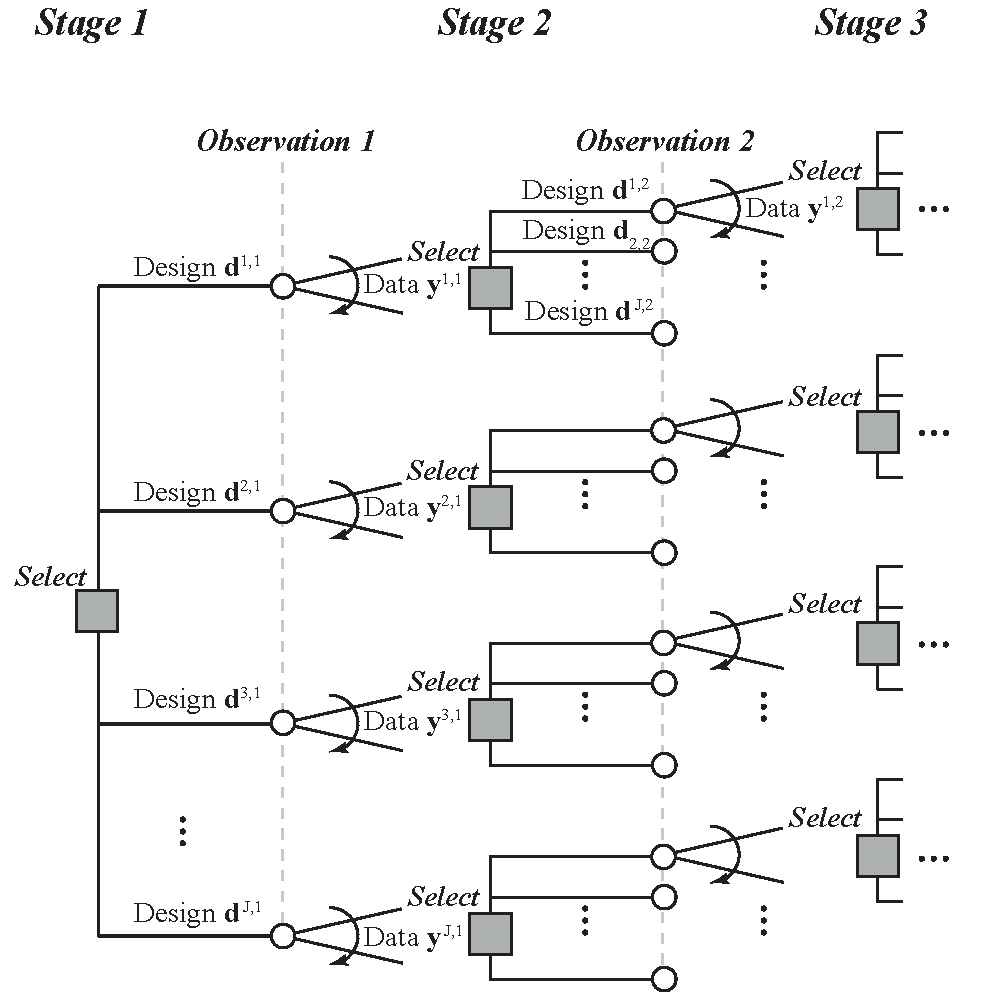
\includegraphics[width=0.85\textwidth]{Figures/sequent_select.pdf}
\caption{Optimal sequential path selection.}\label{fig:PathSelOpt}
\end{figure}
where design choices are indicated by squares while data realizations are indicated by circles. 
%terms this optimal design is defined as
%\begin{equation}\label{opt_crit}
%    \bd^* = \mbox{argmin}_{d^{j,1}} \left\{ \int_{\by^{j,1}} \mbox{argmin}_{d^{j,2}} \left\{ \int_{\by^{j,2}} \ldots \pi(\by^{j,2}|\by^{j,1}) d\by^{j,2} \right\} \pi(\by^{j,1}) d \by^{j,1} \right\},
%\end{equation}
%where $\ldots$ represents the expected variance reduction in the ES under the continued optimal design, which will depend on the data at earlier stages. 
The mathematical expression for the optimal design then involves a
series of intermixed maximisations over designs and integrals over
data. In practice, the optimal solution is intractable because of
the enormous growth over stages (see
e.g. \cite{sucar2015probabilistic} and \cite{powell2016perspectives}).
Instead, we outline heuristic strategies. In terms of notation, let
$\mathcal{Y}^{s-1} =\{d^{j,r}, \by^{j,r} ; r=1,\ldots,s-1 \}$ denote
the data gathered until stage $s-1$, using a selected design
$d^{j,r}$, $r=1,\ldots,s-1$.

%The derived closed-form solutions for the expected IBV are still important building blocks when constructing the sampling designs, as they will be used to score the different adaptive designs. % Efficient
% calculation is important for using adaptive survey designs with
% robotic platforms.
 
\subsection{A Naive Sampling Strategy}
\label{naive}

The simplest heuristic for adaptive sampling is to choose the next
sampling location based on current EPs. The largest variance in
sampling locations indicates higher levels of uncertainty; therefore
one selects the design location with an EP closest to $0.5$.

At stage $s$, based on the currently available data
$\mathcal{Y}^{s-1}$, we fit an updated Gaussian model from
Eq. (\ref{gp_upd}) with mean $\bm^{s-1}=E(\bxi|\mathcal{Y}^{s-1})$
and covariance matrix $\bA^{s-1}=\mbox{Var}(\bxi|\mathcal{Y}^{s-1})$.
The next stage of measurements $\by^{j,s}$ can be gathered with
design $d^{j,s}$, $j=1,\ldots,J$. The {\it{naive}} strategy then
selects the design according to:
\begin{eqnarray}\label{critNaive}
    d^{*,s} &=& \mbox{argmin}_{j \in \{1,\ldots,J\}} |p(\bx_{d^{j,s}};\mathcal{Y}^{s-1})-0.5|, \\
    p(\bx;\mathcal{Y}^{s-1}) &=& P(\xi_T(\bx) \leq t_T, \xi_S(\bx) \leq t_S | \mathcal{Y}^{s-1}). \nonumber
\end{eqnarray}
This strategy does not account for the uncertainty in the temperature
or salinity variables, but is instead applicable only if one design (node) has EPs closer to
$0.5$ (see Table \ref{tab:sim_rhoab}, line two). Additionally, this strategy does not
account for spatial correlation. This strategy lacks memory of where
it has been and where the uncertainty has been reduced, and is therefore
susceptible to local minima.

\subsection{Myopic Path Planning}
\label{sec:myopic}

The myopic (greedy) strategy which we present here is optimal if we
imagine taking only one more stage of measurements. In this selection
strategy, there is no anticipation of what the subsequent designs might
offer beyond the first stage.

Based on the currently available data $\mathcal{Y}^{s-1}$, we
fit an updated GP model.  The next stage of measurements
$\by^{j,s}$, can be gathered with design $d^{j,s}$, $j=1,\ldots,J$. The
selected design is then:
\begin{eqnarray}\label{critSEQ}
    d^{*,s} &=& \mbox{argmin}_{j \in \{1,\ldots,J\}} \left\{ V_{m,\mbox{upd,j}} \right\},  \\
V_{m,\mbox{upd}} & \approx & \sum_{\bx \in \mathcal{M}_g} E_{\by^{j,s}|\mathcal{Y}^{s-1}} \left( p(\bx;\mathcal{Y}^{j,s})\left( 1-p(\bx;\mathcal{Y}^{j,s})\right) \right) \Delta, \nonumber \\
    p(\bx;\mathcal{Y}^{j,s}) &=& P(\xi_T(\bx) \leq t_T, \xi_S(\bx) \leq t_S |\by^{j,s},\mathcal{Y}^{s-1}). \nonumber
\end{eqnarray}

Note that this strategy gives a sequential conditional version of the
formula in Eq. (\ref{sur}). Now $\mathcal{Y}^{s-1}$ is available, and
the expectation is with respect to the conditional density
$\pi(\by^{j,s}|\mathcal{Y}^{s-1})$. A similar closed-form calculation
for expected IBV is hence applicable in Eq. (\ref{critSEQ}) using the
updated GP model from stage $s-1$. Once the data is collected for the
best design, the GP model is updated again. The mean $\bm^{s}$ and
covariance matrix $\bA^{s}$ are used to compute the next design at
stage $s+1$, and so on.

Even though this myopic strategy is non-anticipative, it still gives a
reasonable approach for creating designs in many
applications. Moreover, it is easily implemented onboard an AUV,
using an efficient approach for data updating the GP model and the
calculation of the closed-form expected IBV expressions for each
subsequent trajectory.


\subsection{Look-ahead Trajectory Planning}
\label{sec:LA}

We now extend the myopic strategy to a look-ahead strategy, which is
optimal when one can gather only two more stages of measurements. In
addition to the next stage of measurements $\by^{j,s}$, this
look-ahead strategy, anticipates the subsequent design $j_2$ with
data $\by^{j_2,s+1}$ when choosing the current design $d^{j,s}$.  The
selected design is:
\begin{eqnarray}\label{critLA}
    d^{*,s} &=& \mbox{argmin}_{j \in \{1,\ldots,J\}} \left\{ U_{la,\mbox{upd,j}} \right\},  \\
    U_{la,\mbox{upd},j} & = &  E_{\by^{j,s}|\mathcal{Y}^{s-1}} \left\{ \mbox{argmin}_{j_2 \in \{1,\ldots,{J}_2\}} \left[ V_{la,\mbox{upd},j_2} \right] \right\}, \nonumber \\
V_{la,\mbox{upd},j_2} & \approx & \sum_{\bx \in \mathcal{M}_g} E_{\by^{j_2,s+1}|\mathcal{Y}^{j,s}} \left\{ p(\bx;\mathcal{Y}^{j,s+1})\left( 1-p(\bx;\mathcal{Y}^{j,s+1})\right) \right\} \Delta, \nonumber \\
    p(\bx;\mathcal{Y}^{j,s+1}) &=& P(\xi_T(\bx) \leq t_T, \xi_S(\bx) \leq t_S |\by^{j_2,s+1},\mathcal{Y}^{j,s}). \nonumber
\end{eqnarray}
Here, $\mathcal{Y}^{j,s}=\{\by^{j,s},\mathcal{Y}^{s-1}\}$ and
$\mathcal{Y}^{j,s+1}=\{\by^{j_2,s+1},\mathcal{Y}^{j,s}\}$ represent
the sets of data variables, and the expectations are calculated with respect to
the conditional densities $\pi(\by^{j,s}|\mathcal{Y}^{s-1})$ and
$\pi(\by^{j_2,s+1}|\by^{j,s},\mathcal{Y}^{s-1})$.

We solve the
first expectation by Monte Carlo sampling of data $\by^{j,s}$ from its
conditional distribution. For each of these data samples, the second expectation
is solved using the closed-form expressions for expected IBV from
Section \ref{sec:sur}.

Even though the strategy looks at two sampling stages, it is only used to find
the current best design. When data are collected, the GP model is
updated, and the mean $\bm^{s}$ and covariance matrix $\bA^{s}$ are
used to compute the next design at stage $s+1$, now anticipating what
stage $s+2$ could offer, and so on.

This look-ahead approach is much more computationally demanding than
the myopic strategy, so for practical implementation, we prune paths
in the evaluation of Eq. (\ref{critLA}). This means that we do not
compute all possible branches of the first two stages, as they are
indicated in Fig. \ref{fig:PathSelOpt}. Instead, we use the myopic
strategy to rank the three best designs following the first stage alone, and
for each of these preferred designs, we undertake the look-ahead calculations.

\section{Simulation study}
\label{sec:simulations}

We now study the properties of
the different static and sequential survey designs in a realistic
simulated case that emulates the spatial properties of a river plume interacting with coastal water.

\subsection{Modeling}

We use a bivariate GP model for temperature and salinity, where we
specify the mean:
\begin{equation}\label{m}
    \bmu(\bx)=E 
    \begin{bmatrix}
    \xi_T(\bx) \\
    \xi_S(\bx) 
    \end{bmatrix}=\begin{bmatrix} \mu_{T}(\bx)\\
\mu_{S}(\bx)
\end{bmatrix} 
= \begin{bmatrix} \beta_{T,0} + \beta_{T,1} x_{\mbox{West}} \\
\beta_{S,0} + \beta_{S,1} x_{\mbox{West}}
\end{bmatrix}.
\end{equation}
This situation
mimics that of a river mouth opening from the south, with the water
masses pulled to the east. The regression parameters are  $\beta_{T,1}=0.065$ and
$\beta_{S,1}=0.1$ for the slopes with west coordinate, and $\beta_{T,0}=5.8$
and $\beta_{S,0}=29.0$ for the intercept at a chosen reference map coordinate.

%The prior assumption used by the agent are $\tilde{\beta_{T,1}}=0.085$ and $\tilde{\beta_{S,1}}=0.138$, which assumes that the process is centered. 

The covariance is assumed to be stationary and separable for the two variables. 
The $2 \times 2$ pointwise covariance matrix is set to:
\begin{equation}\label{v0}
\bSigma(\bx)=\mbox{Var} 
\begin{bmatrix}
    \xi_T(\bx) \\
    \xi_S(\bx) 
    \end{bmatrix}=
\begin{bmatrix}
0.25^2 & 0.6 \cdot 0.25^2 \\
0.6 \cdot 0.25^2 & 0.25^2
\end{bmatrix}.
\end{equation}
The spatial correlation is of a Matern type \kc{cite or define}:
\begin{equation}\label{v}
\small
\mbox{Corr} 
\left(
\begin{bmatrix}
    \xi_T(\bx) \\
    \xi_S(\bx) 
    \end{bmatrix},
    \begin{bmatrix}
    \xi_T(\bx') \\
    \xi_S(\bx') 
    \end{bmatrix}
    \right)
    = \begin{bmatrix}
1 & 0.6  \\
0.6  & 1
\end{bmatrix}(1+\phi h)\exp (-\phi h),
\end{equation}
where $h=\sqrt{||\bx-\bx'||^2}$ and $\phi=0.3$ indicates an effective correlation range of about $1200$ m. 
%Figure \ref{fig:stat_design} shows the contour lines for the EP for the reference. We notice the trend of increasing salinity and temperature to the west.  
One realization of the random fields representing salinity and
temperature is shown in Fig. \ref{fig:true_temp} and
\ref{fig:true_sal}. The true ES is a realization from this model as shown
in Fig. \ref{fig:ESet}.

\begin{figure}[!ht]
  \centering
  \subfigure[Simulated temperature.]{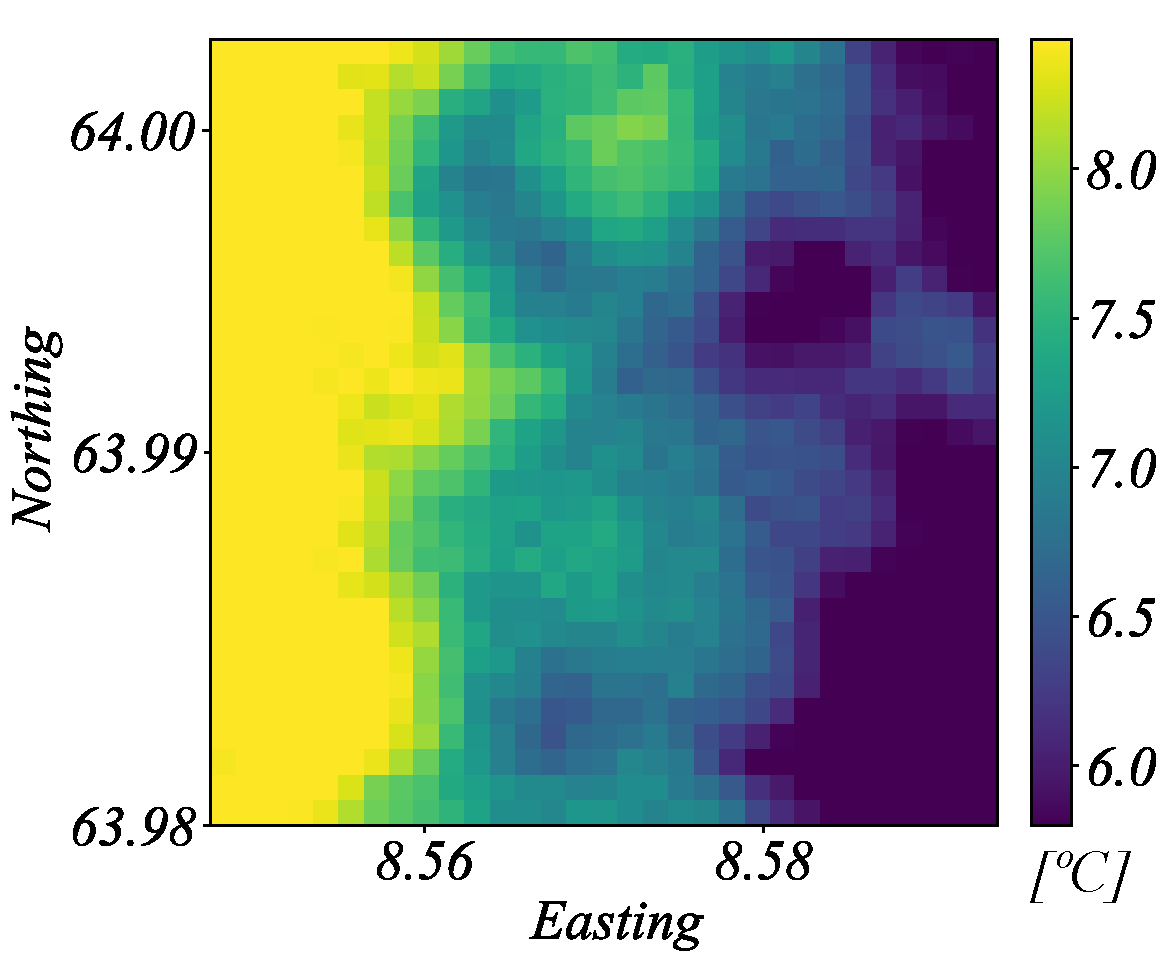
\includegraphics[height = 0.40\textwidth]{Figures/sim/true_temp.pdf}\label{fig:true_temp}}
  \hfill
  \subfigure[Simulated salinity.]{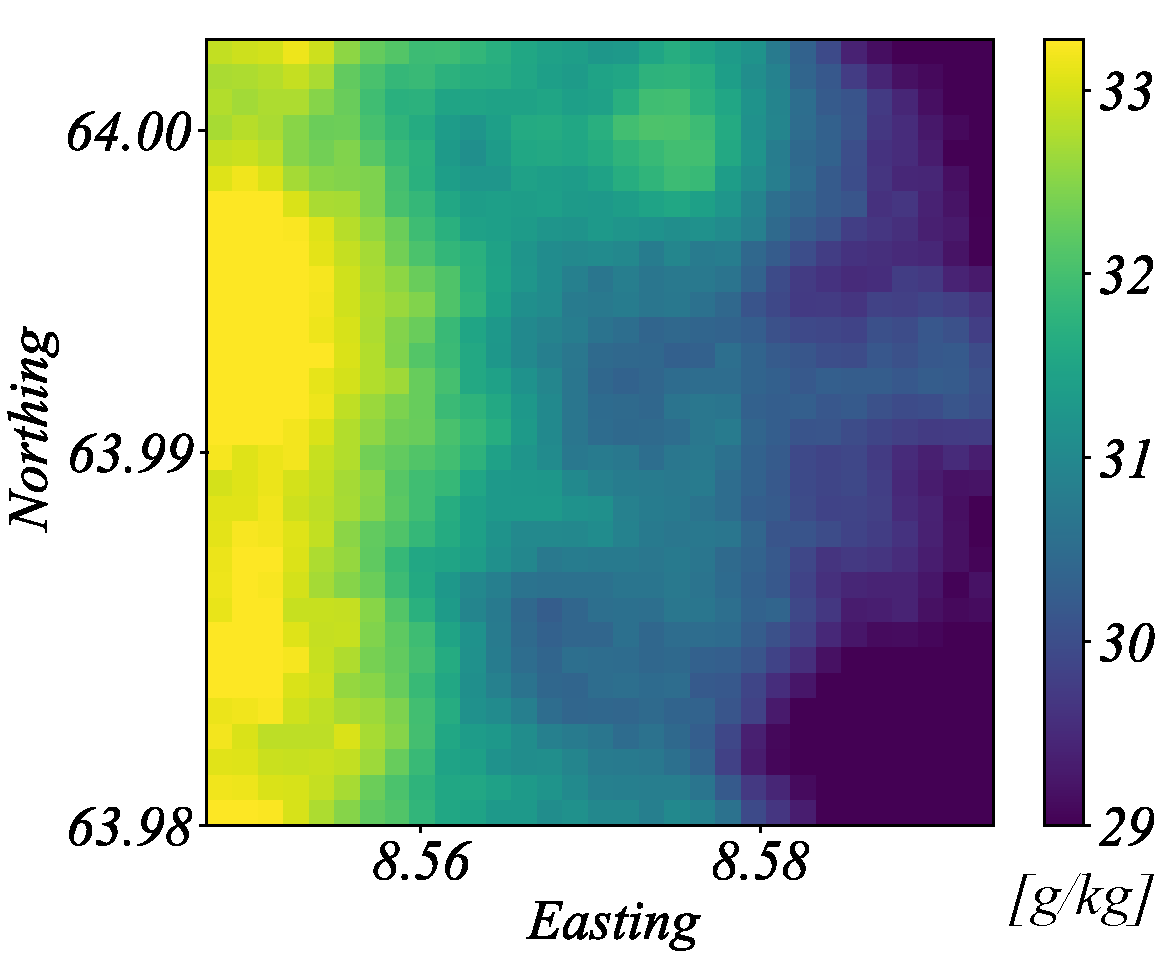
\includegraphics[height = 0.40\textwidth]{Figures/sim/true_sal.pdf}\label{fig:true_sal}}
  \hfill
  \subfigure[Excursion set given the realization of temperature and salinity.]{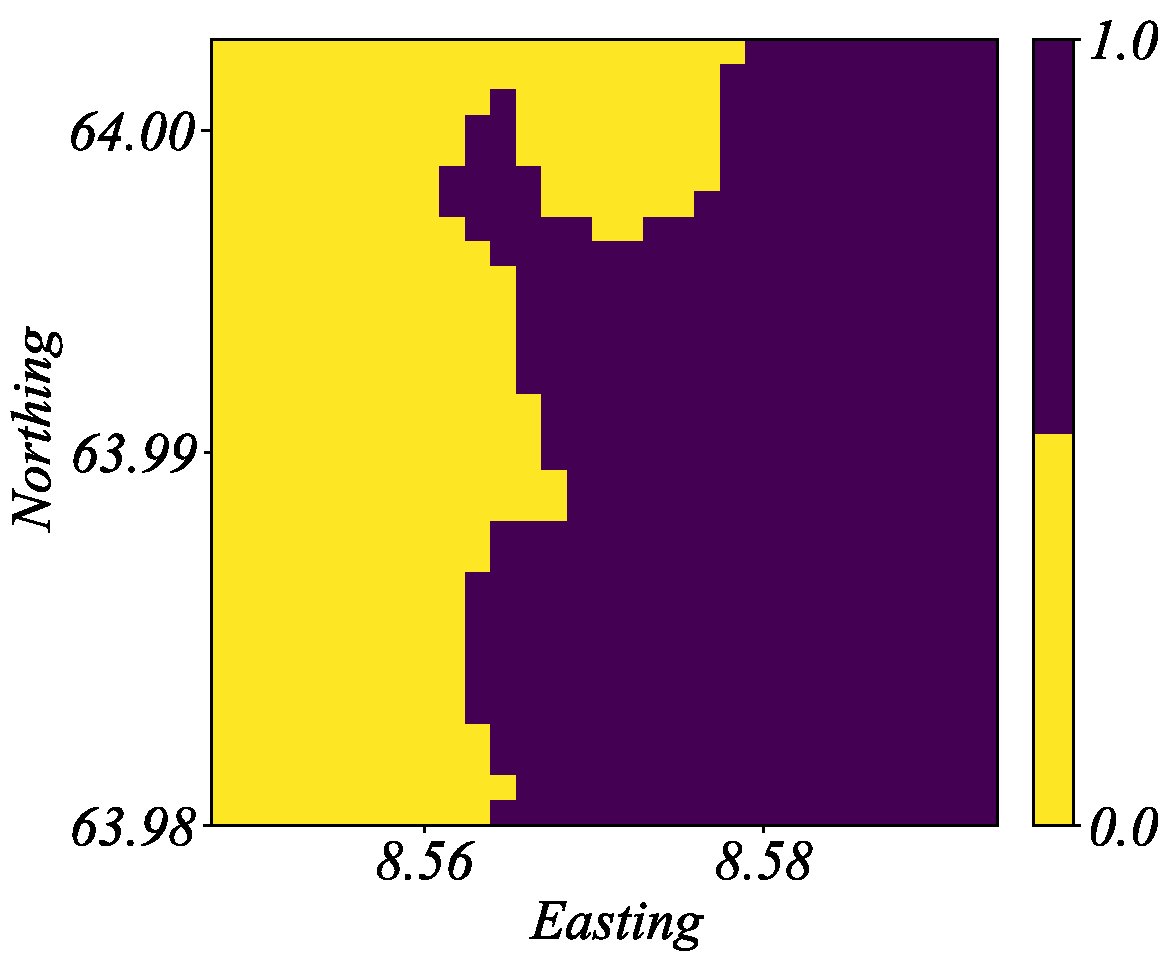
\includegraphics[height = 0.40\textwidth]{Figures/sim/es_ts_true.pdf}\label{fig:ESet}}
  \hfill
  \subfigure[Excursion probabilities given collected data using the
  `static\_north" strategy.]{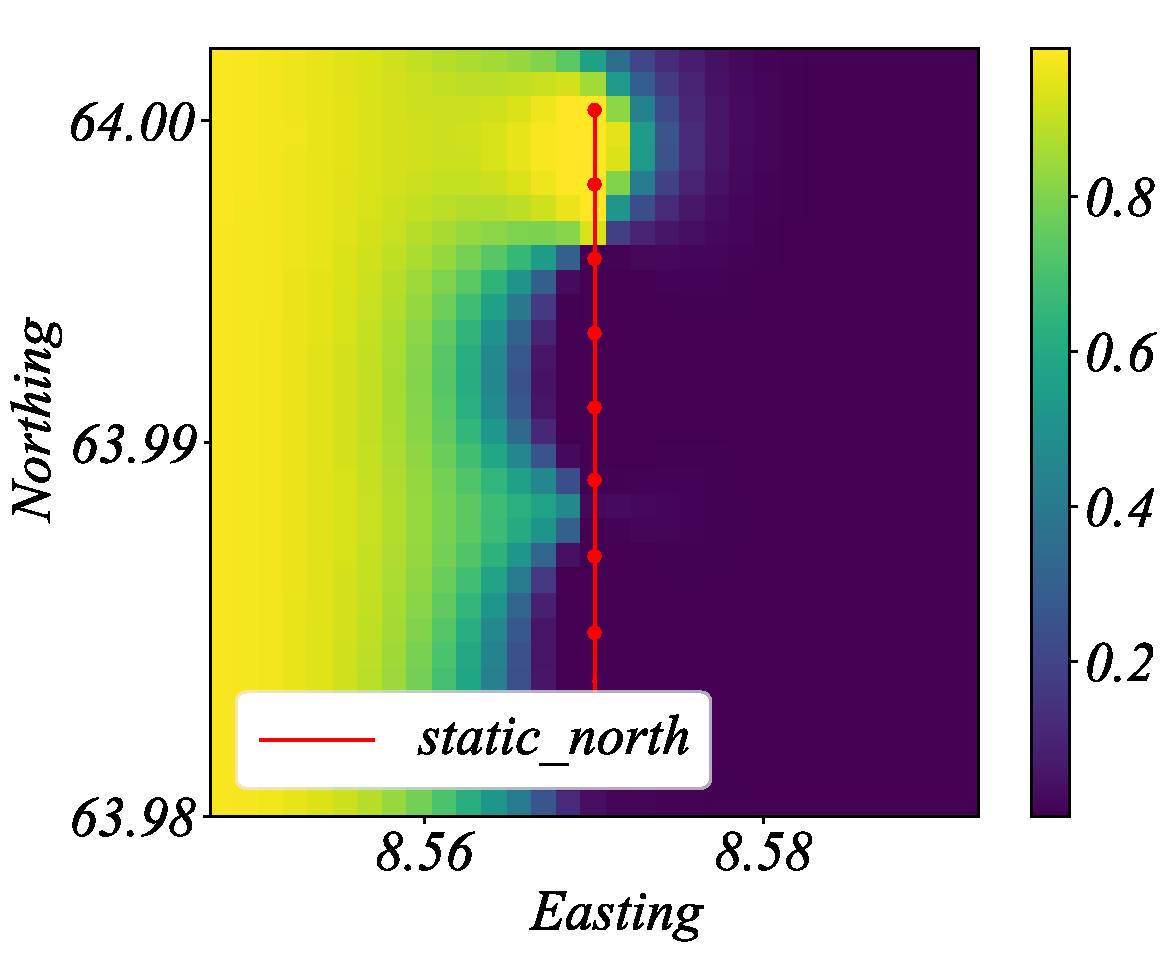
\includegraphics[height = 0.40\textwidth]{Figures/sim/es_ts_posterior.pdf}\label{fig:Eprob}}
  \caption{\ref{fig:true_temp} and \ref{fig:true_sal} show
    a realisation of the simulated temperature and salinity fields. The associated ES is in \ref{fig:ESet}, while 
    \ref{fig:Eprob} shows the estimated EPs after
    performing data collection along the static N-S survey line.} 
\label{fig:realisations}
\end{figure}

\subsection{Static and Sequential Sampling Designs}\label{sec:sampling_designs}

%Three different designs are considered as indicated in Figure \ref{fig:stat_design}. 
%\begin{figure}[h!]
%\centering
%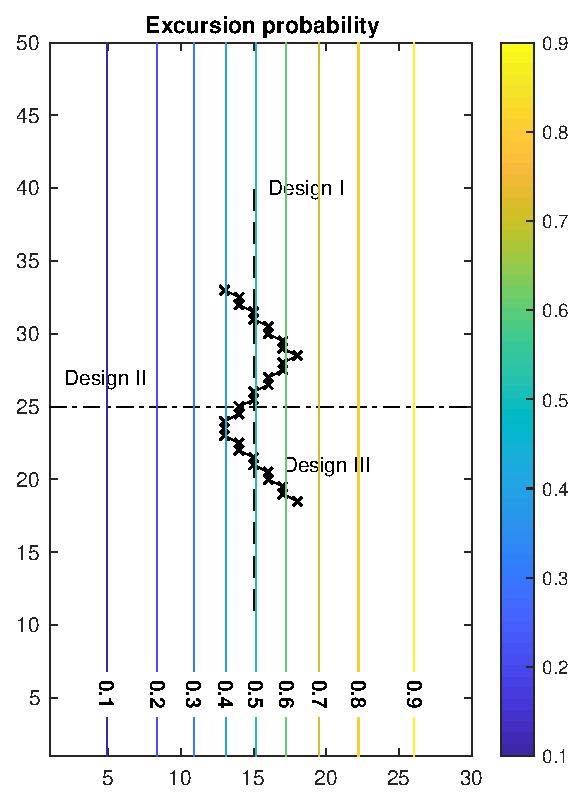
\includegraphics[width=0.65\textwidth]{Figures/Des3.eps}
%\caption{Three different static survey designs plotted on the initial EP.}\label{fig:stat_design}
%\end{figure}
%In this display the designs are plotted along with the prior probability contours of the ES for the reference parameter inputs. 

We compare three different static designs denoted
\textit{static\_north}, \textit{static\_east}, and
\textit{static\_zigzag} with the three described sequential approaches
\textit{naive}, \textit{myopic}, and \textit{look-ahead}. The static sampling paths are pre-determined and cannot be altered and represent the pre-planned strategies used in most current AUV
operational survey designs.

For a fixed survey length, a closed form expression for the expected IBV is available as in Eq. \eqref{sur}. However, for the sequential approaches this is not the
case. For comparison the properties are therefore evaluated using
Monte Carlo sampling over several replicates of realizations from the model while conducting simulated sequential surveys for each
one. Fig. \ref{fig:Eprob} shows the conditional EP, given data
gathered along the north-south survey lines in these figures. In the
Monte Carlo replicates, such results are repeatedly computed to
approximate the expected IBV. We also compare predictive performance
measured by root mean square error (RMSE) for temperature and salinity
estimates as well as also the variance reduction in these two variables. It is
important to note that the objective function used by the agent is
focused on reducing the expected IBV, but we nevertheless expect that
we will achieve good predictive performance for criteria such as RMSE
as well. Another non-statistical criteria that is important for
practical purposes is the computational time needed for the strategy,
as this will impact the performance for an embedded system.

%\begin{figure}[h!]
%\centering
%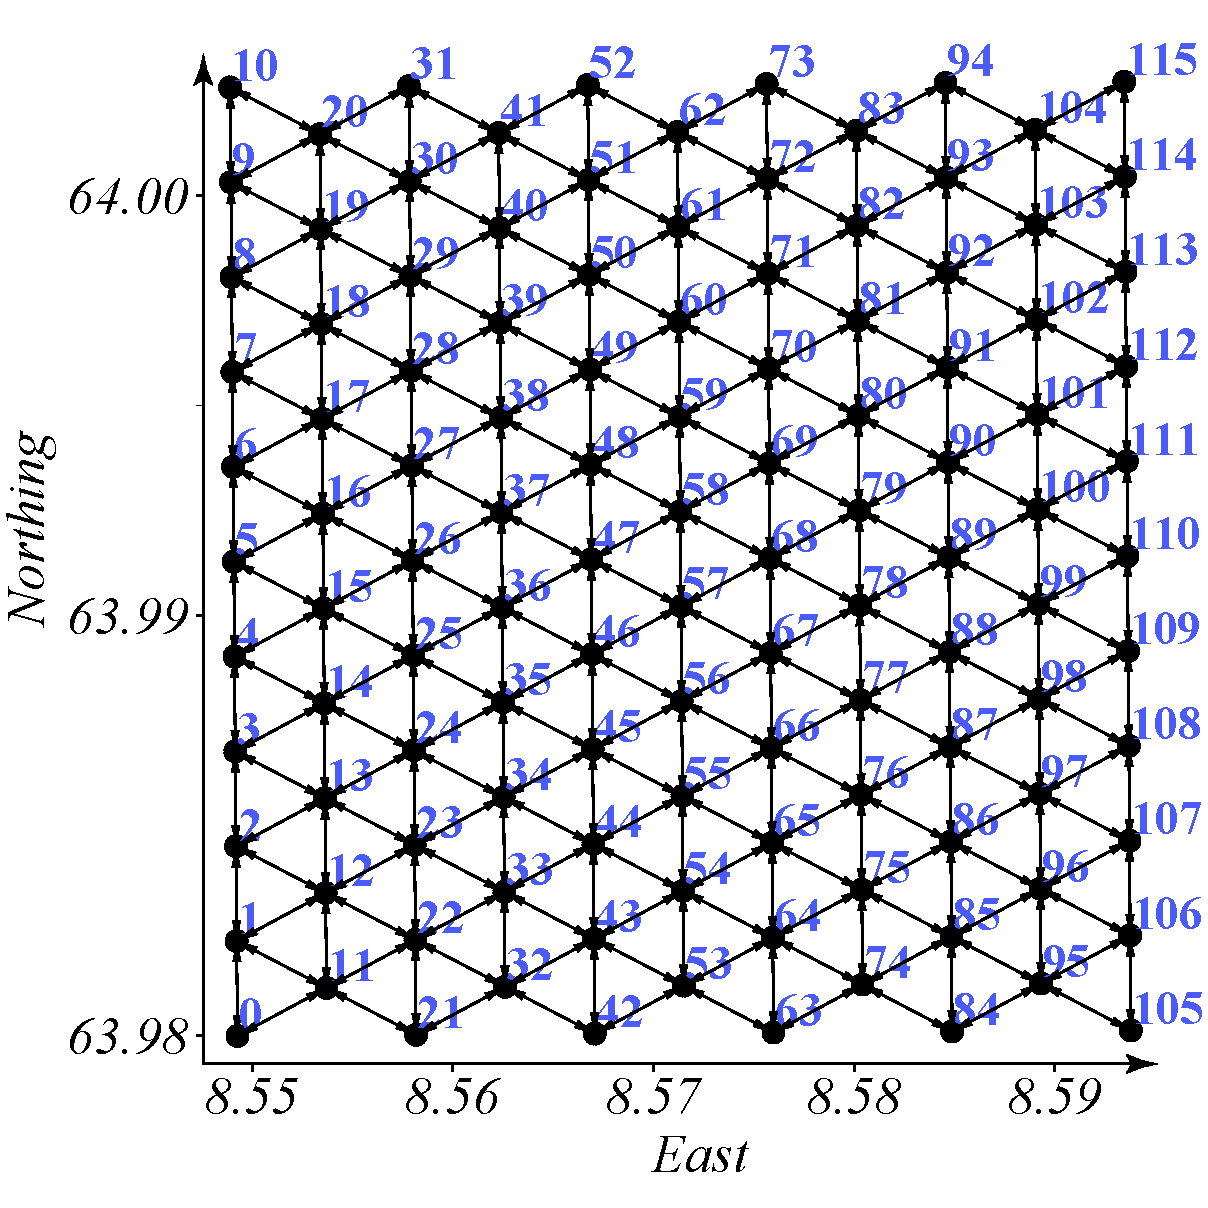
\includegraphics[width=0.50\textwidth]{Figures/sim/wp_graph_paper.pdf}
%\caption{The equilateral waypoint graph used to discretize the
%  trajectory choices over the $31\times31$ grid used to discretize the GP.}
%\label{fig:wp_graph}
%\end{figure}

\begin{figure}[!h] 
\centering 
\subfigure[The waypoint graph.]{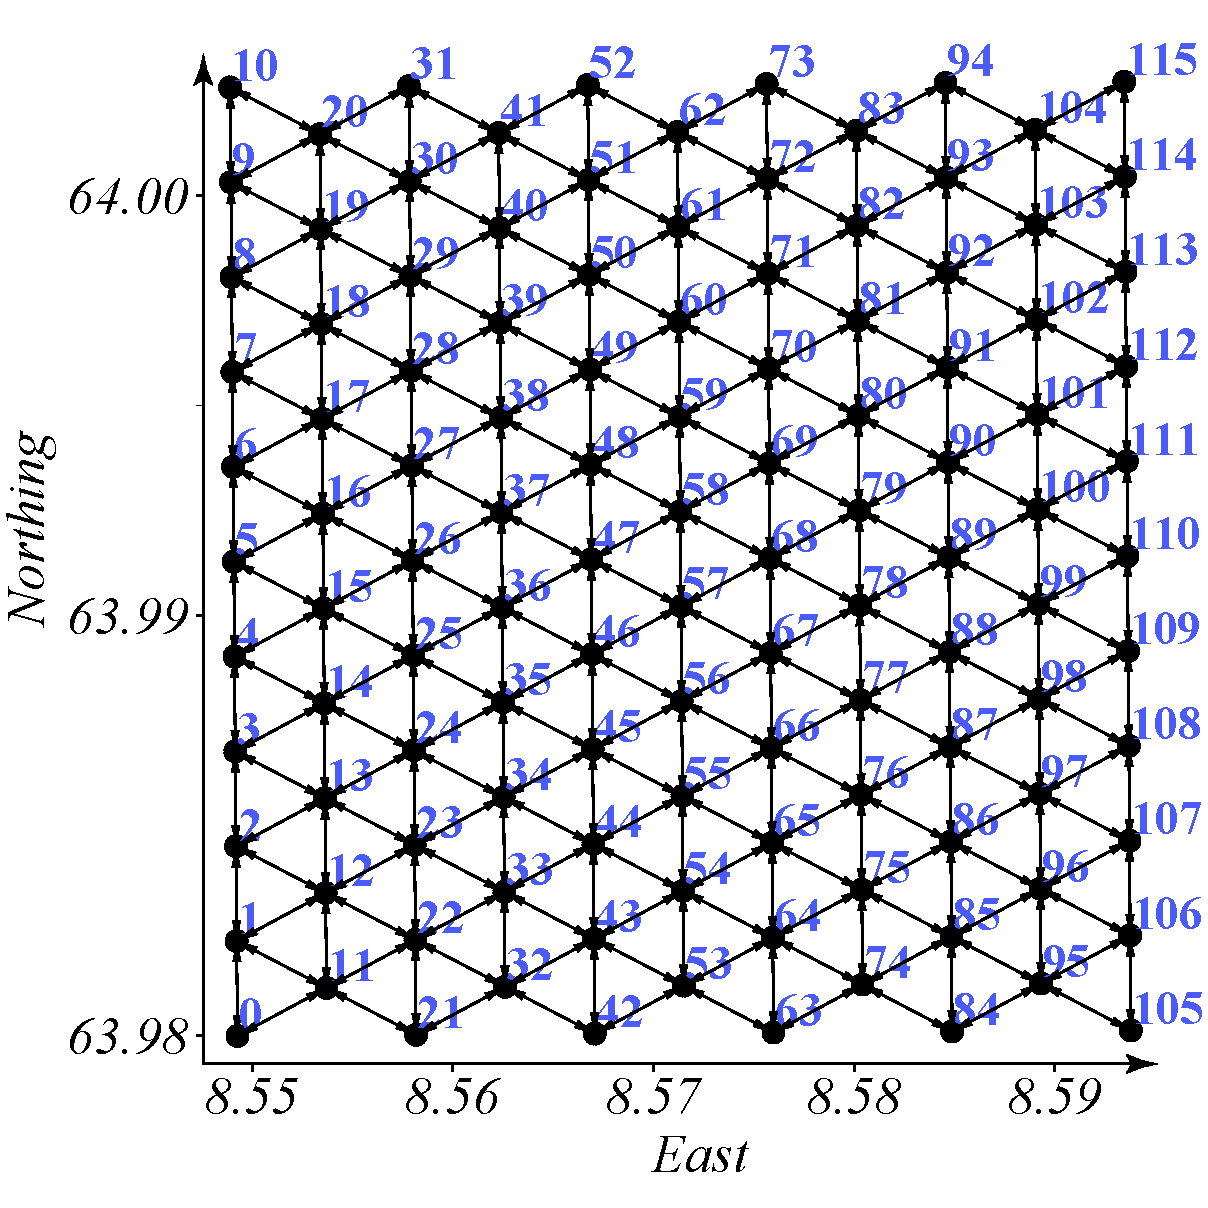
\includegraphics[width =
0.49\textwidth]{Figures/sim/wp_graph_paper.pdf}\label{fig:wp_graph_a}}
\hfill
\subfigure[The waypoint graph in 3D.]{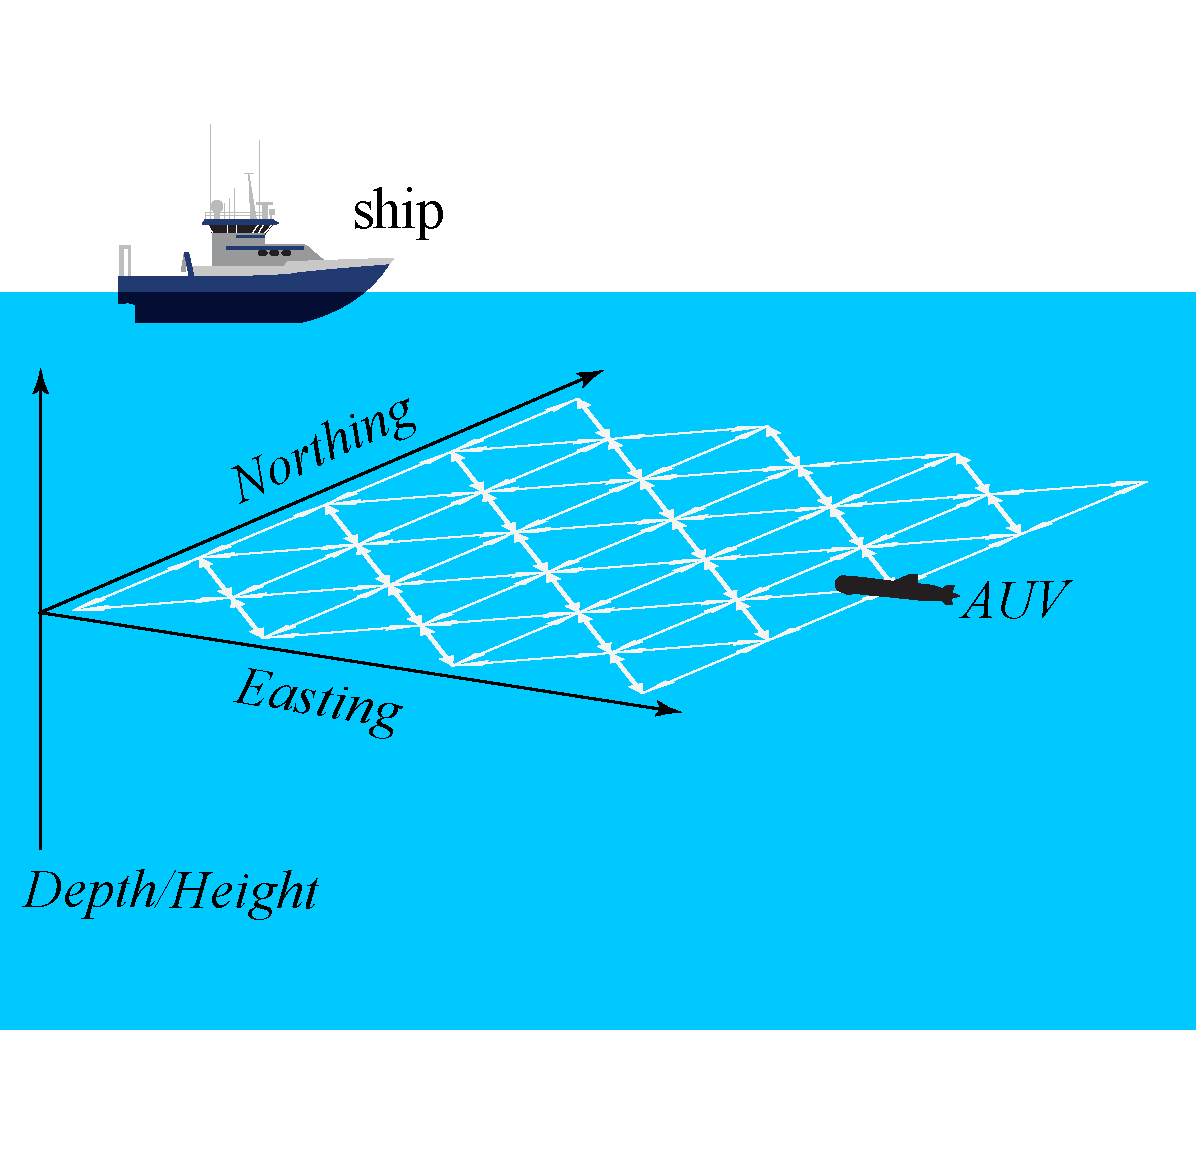
\includegraphics[width =
0.49\textwidth]{Figures/sim/wp_graph_3d.pdf}\label{fig:wp_graph_b}}
\caption{\ref{fig:wp_graph_a} The equilateral waypoint graph used to discretize the
trajectory choices over the $31\times31$ grid used to discretize the GP.
\ref{fig:wp_graph_b} The waypoint grid shown in a 3D environment.}
\label{fig:wp_graph}
\end{figure}

Each strategy is conducted on an equilateral grid as shown in
Fig. \ref{fig:wp_graph}. The sequential sampling agent starts at the
center East-West coordinate at the southern end of the domain (node
53). The AUV moves along edges in the waypoint graph while the vehicle
gathers measurements. The data is assimilated into the GP model before
an evaluation of the next node to sample is conducted at the end of
the edge.

\subsection{Simulation Results}

A total of 100 replicate simulations were conducted with all
strategies. The results are shown in Fig. \ref{fig:sim_results}, where
the different criteria are plotted as a function of survey
distance. Fig. \ref{fig:avg_ev} shows the resulting drop in IBV for
each of the six strategies. IBV reduction occurs most under the
\textit{myopic} and \textit{look-ahead} strategies, each performing
almost equally; this is expected as the two criteria
(Eq. \eqref{critSEQ} and \eqref{critLA}) are sensitive to differences
in IBV. The \textit{static\_north} design also does well here because
the path is parallel to the boundary between the water masses.

\begin{figure}[h!]
  \centering
  % \subfigure[Excursion set variance $E_{\by}(p[1-p])$.]{\label{fig:avg_ev}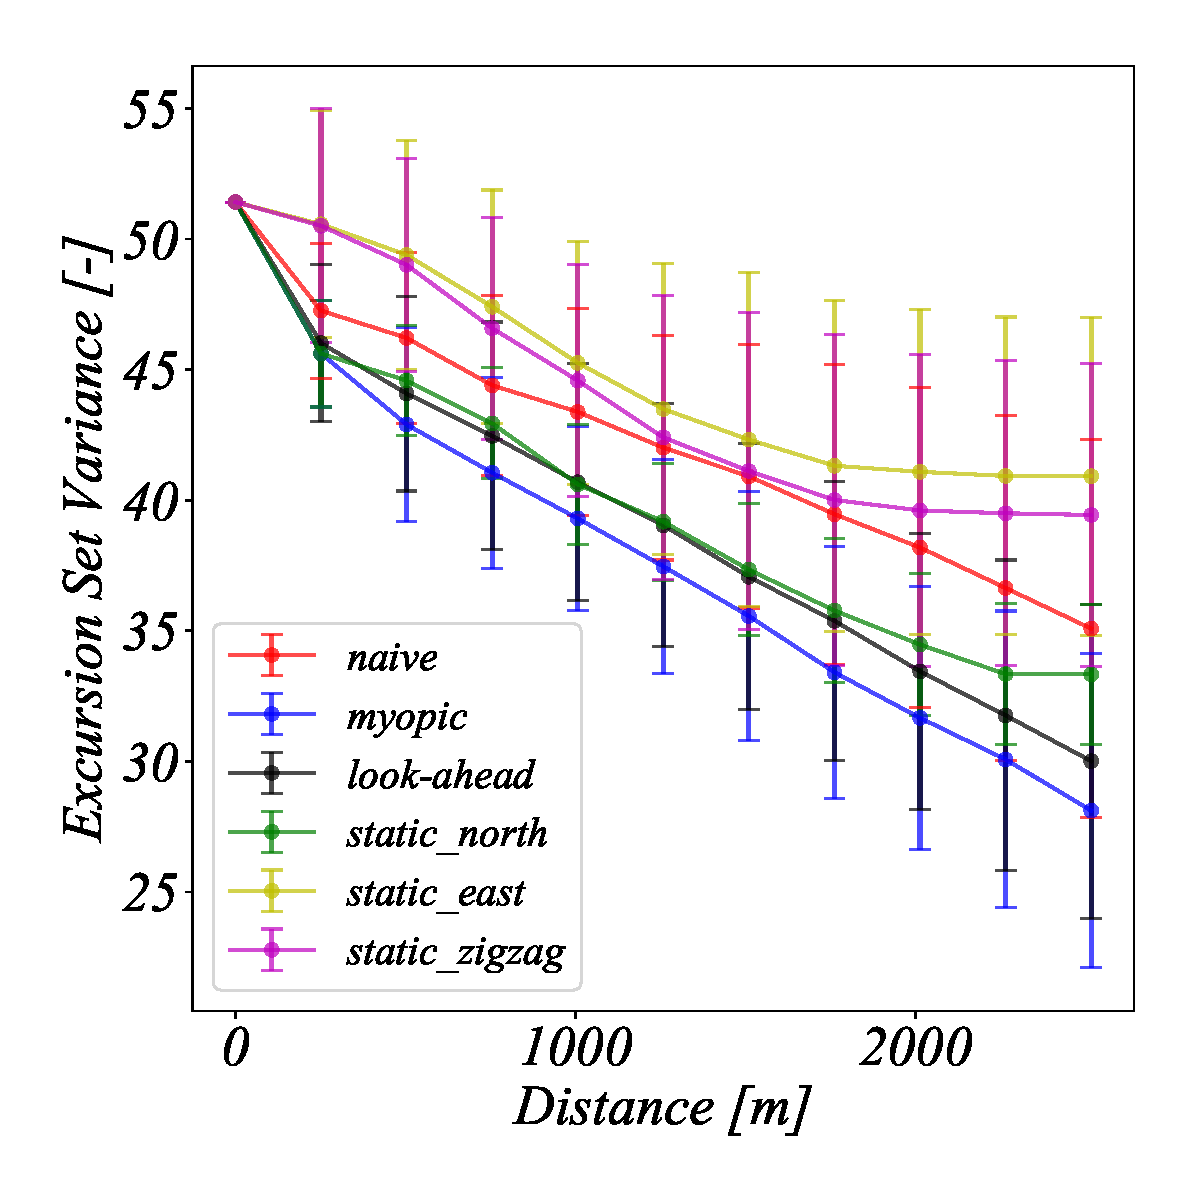
\includegraphics[height=0.49\textwidth]{Figures/sim/avg_EV.pdf}}
  \subfigure[IBV.]{\label{fig:avg_ev}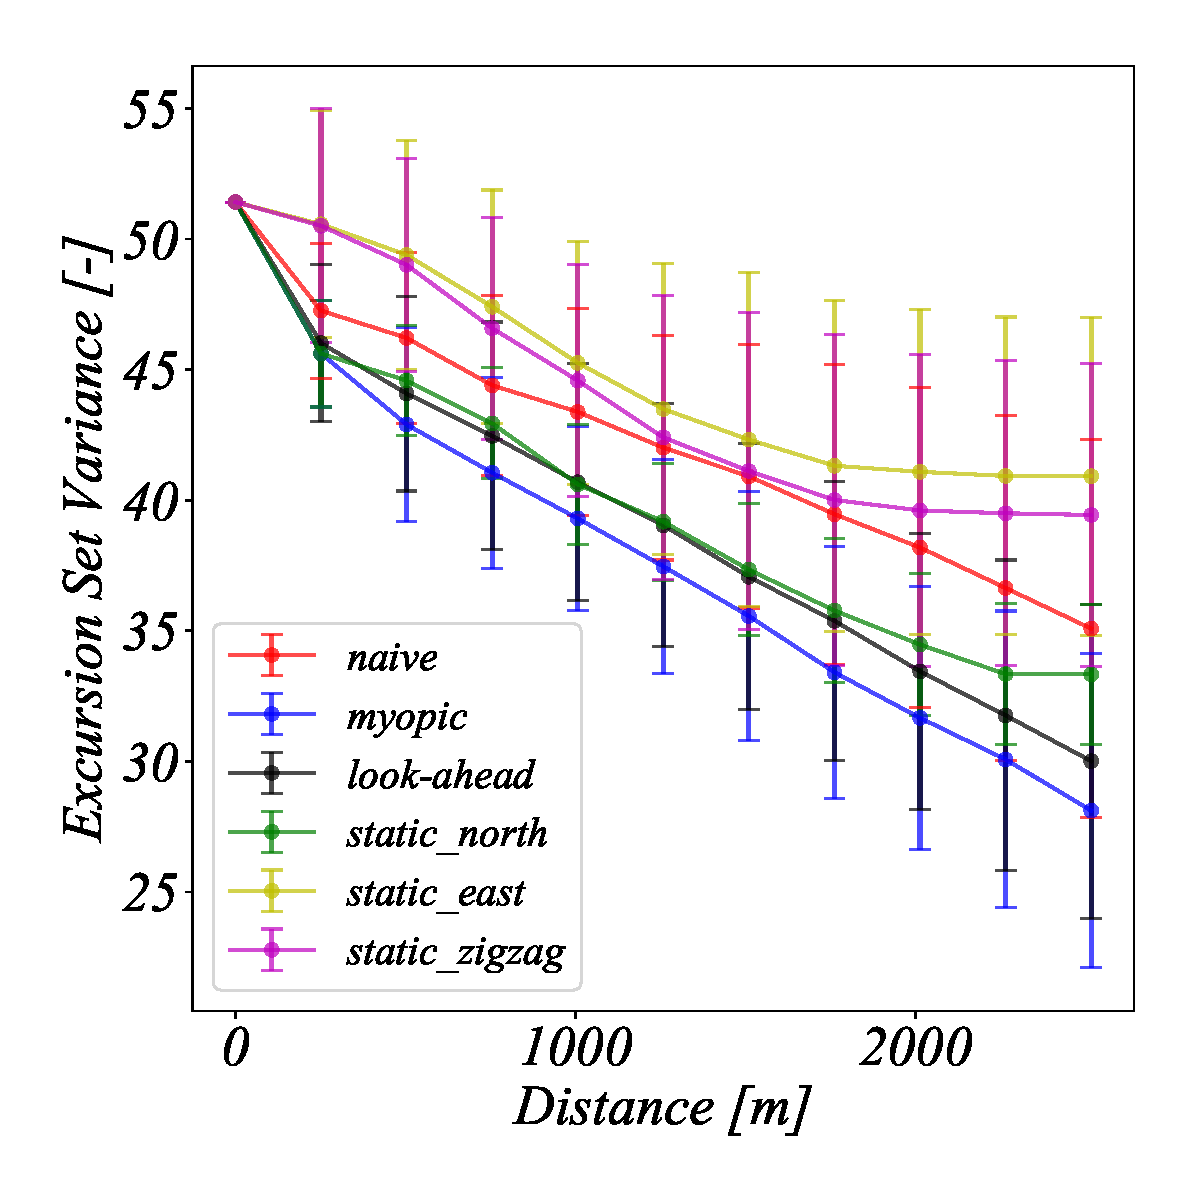
\includegraphics[height=0.49\textwidth]{Figures/sim/avg_EV.pdf}}
  \hfill
  \subfigure[RMSE between estimated field and truth.]{\label{fig:avg_rmse}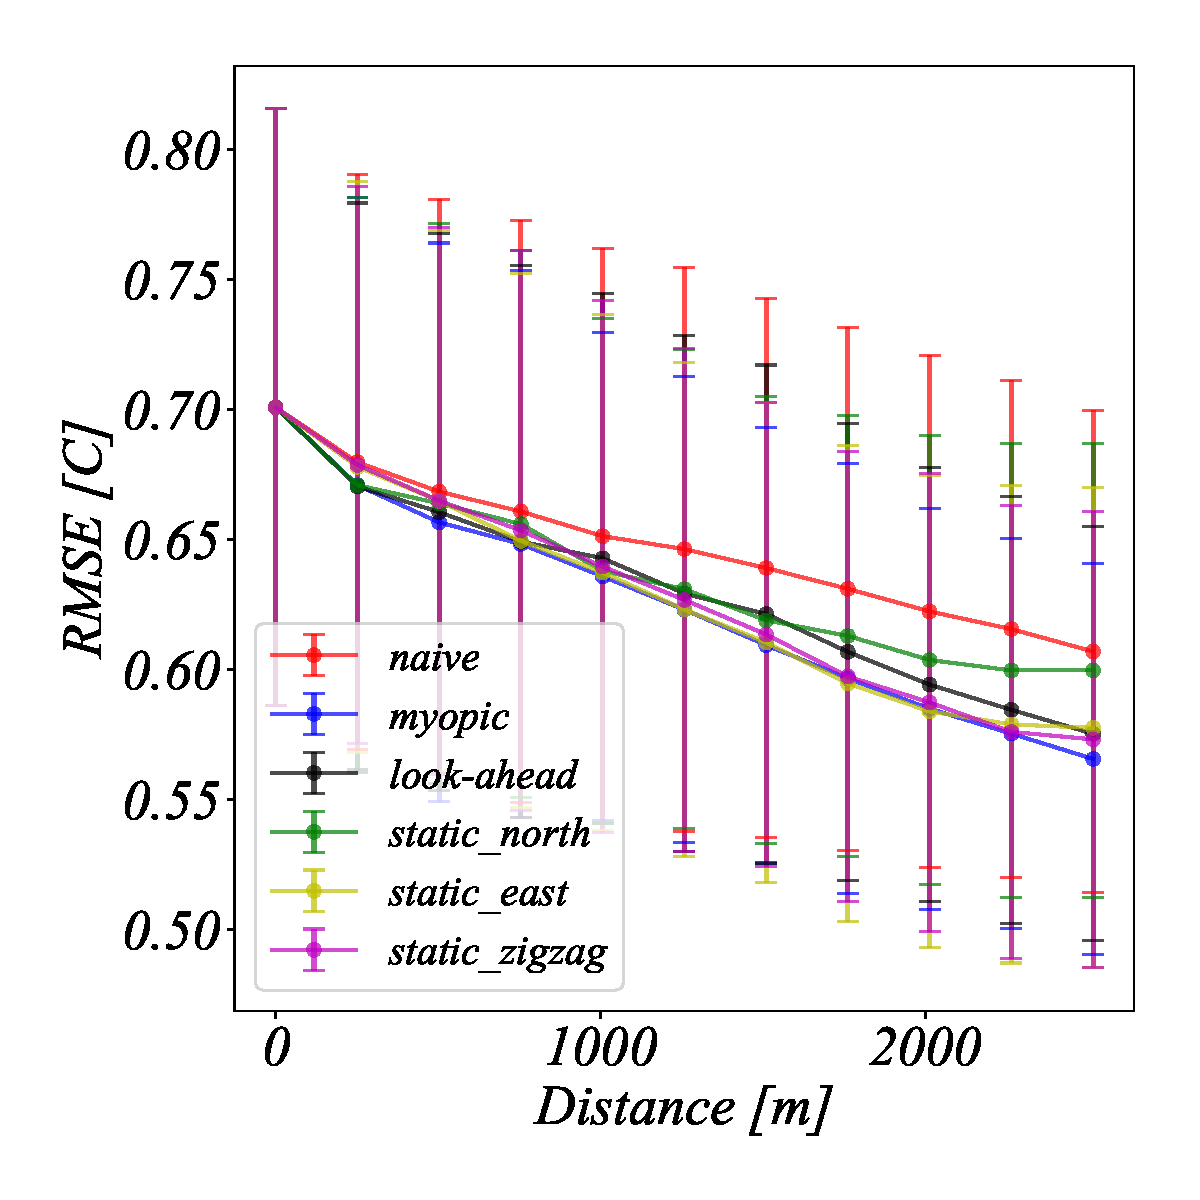
\includegraphics[height=0.49\textwidth]{Figures/sim/avg_RMSE.pdf}}
  \hfill 
  \subfigure[Explained variance $\bR^{2}$.]{\label{fig:avg_r2}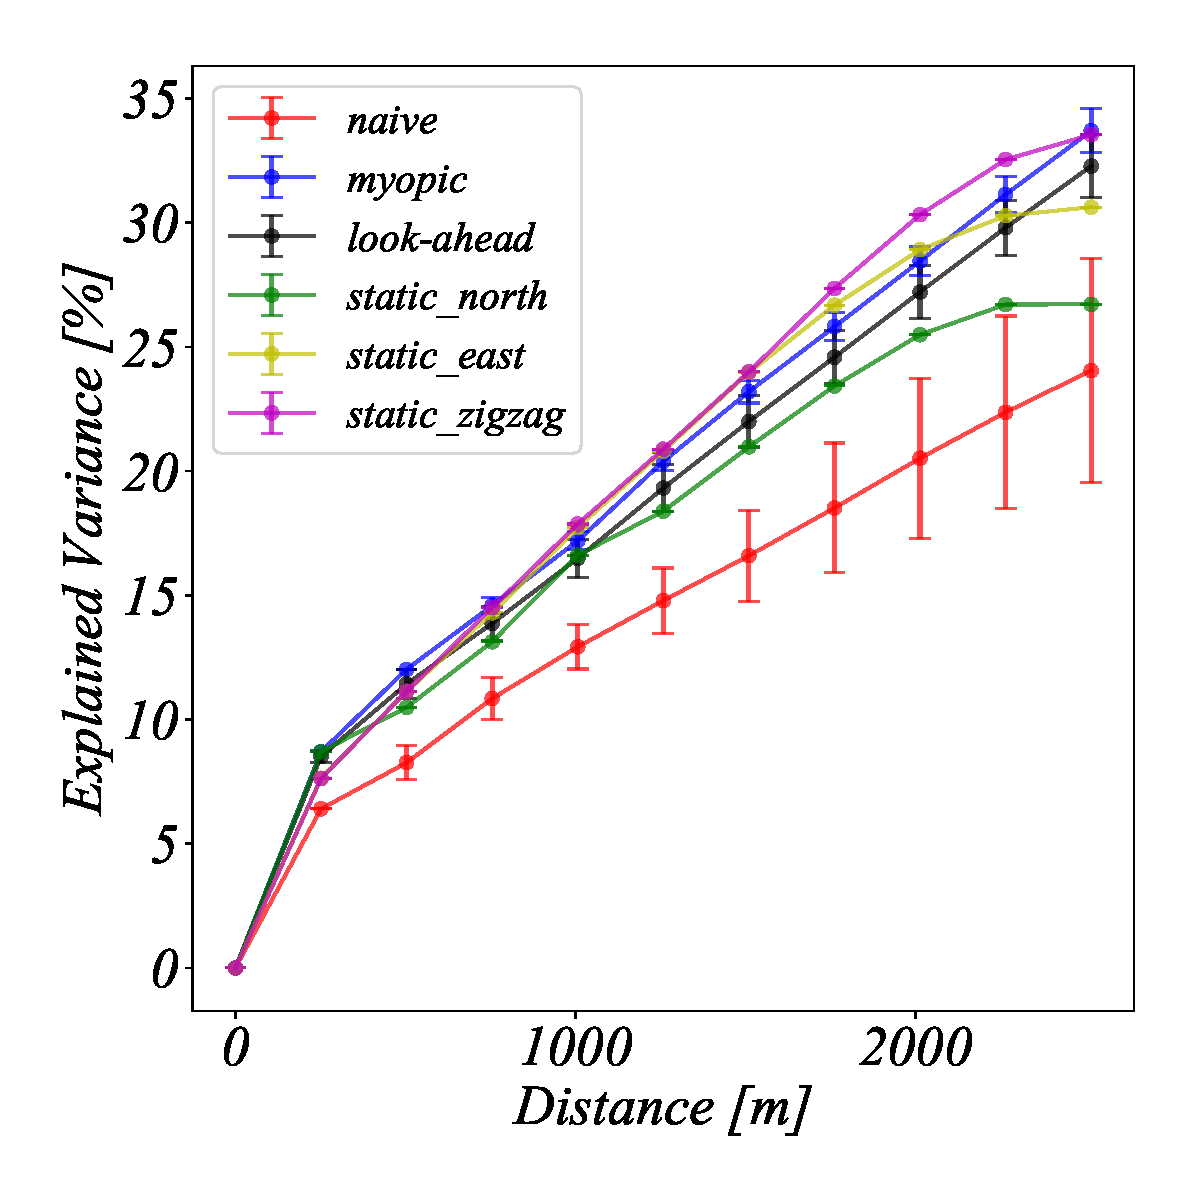
\includegraphics[height=0.49\textwidth]{Figures/sim/avg_R2.pdf}}
  \hfill 
  \subfigure[Time used to do inference.]{\label{fig:avg_time}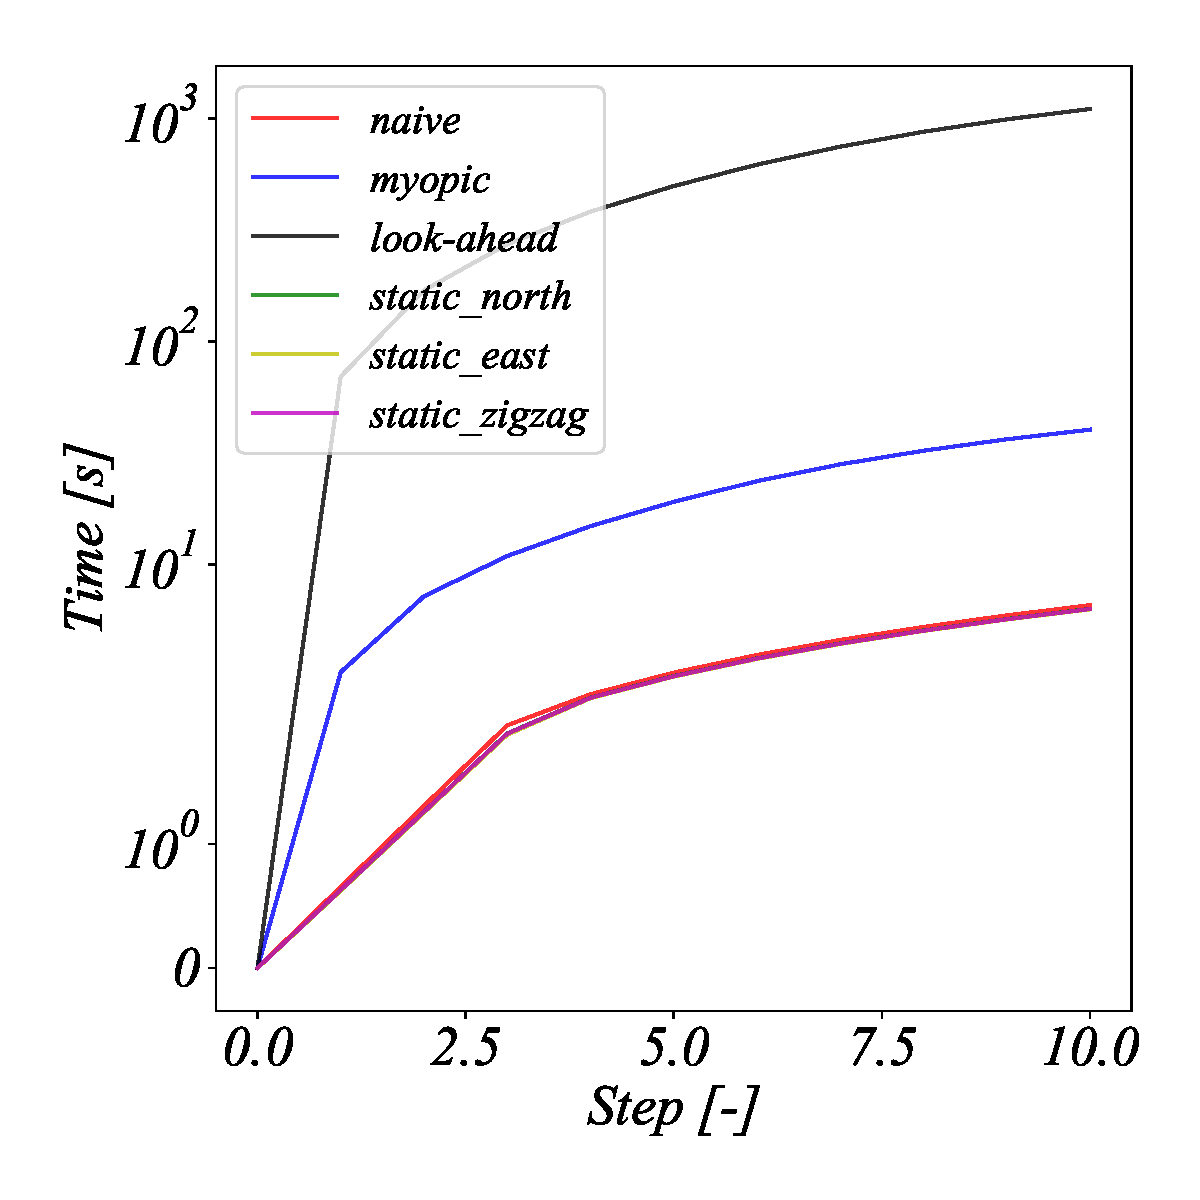
\includegraphics[height=0.49\textwidth]{Figures/sim/avg_Time.pdf}}
\caption{Simulation results from 100 replicate simulations for 10
  sampling choices/stages on the grid.} 
\label{fig:sim_results}
\end{figure}

Fig. \ref{fig:avg_rmse} and \ref{fig:avg_r2} show the resulting drop
in RMSE and increase in explained variance, respectively. Both
\textit{myopic} and \textit{look-ahead} strategies perform well here,
but some of the \textit{static\_east} and \textit{static\_zigzag} also
achieve good results because they are pre-determined to cover large
parts of the domain without re-visitation. Sequential strategies
targeting IBV will sometimes not reach similar coverage, as
interesting data may draw the path into twists and turns. There is
relatively large variety in the replicate results as indicated by the
vertical lines. Nevertheless, the ordering of strategies is similar.

\begin{figure}[!b]
  \centering
  \subfigure[Look-ahead]{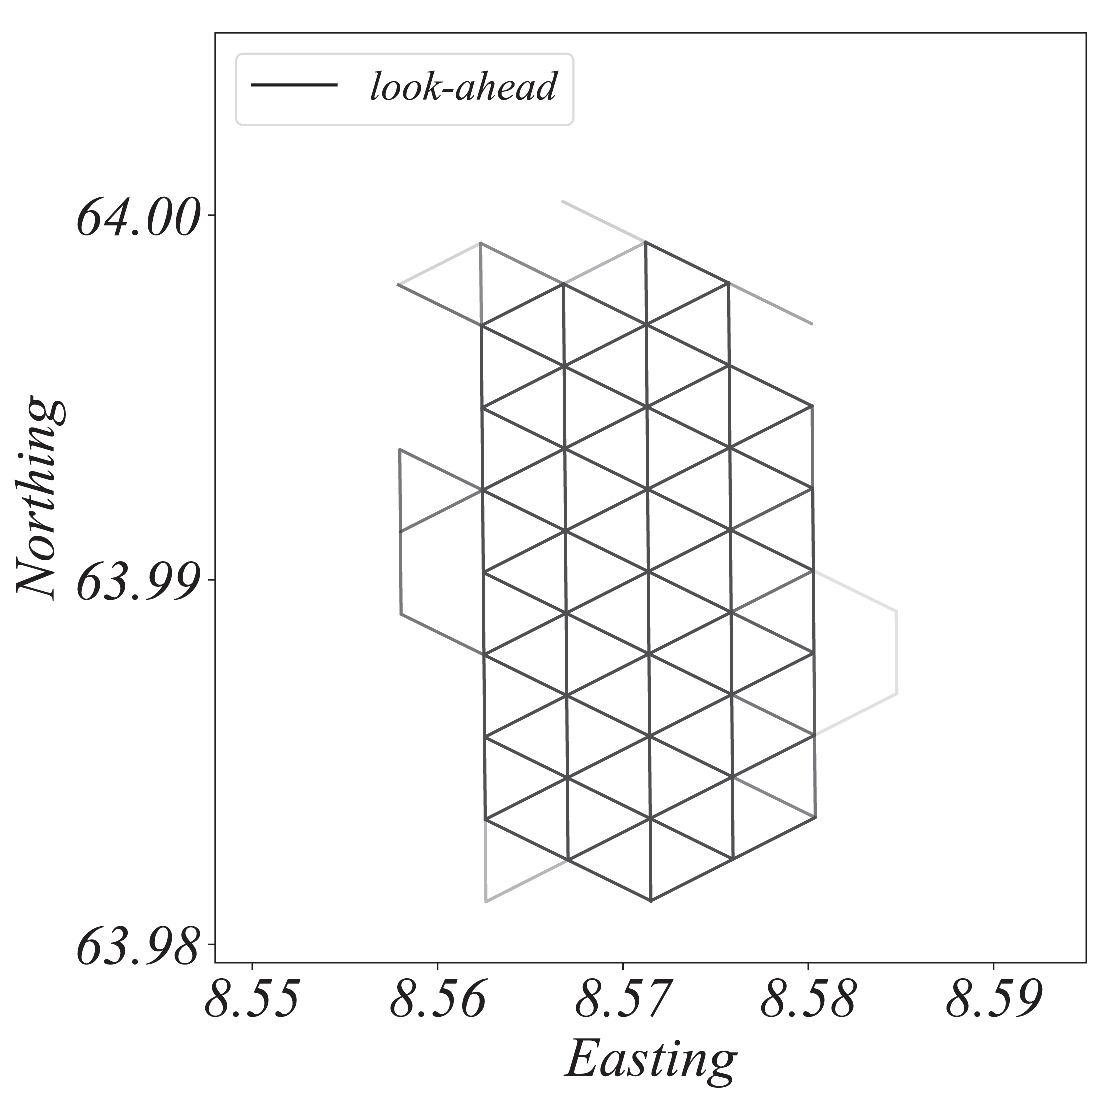
\includegraphics[height = 0.46\textwidth]{Figures/sim/route_look-ahead.pdf}\label{fig:avg_look-ahead}}
  \hfill
  \subfigure[Myopic]{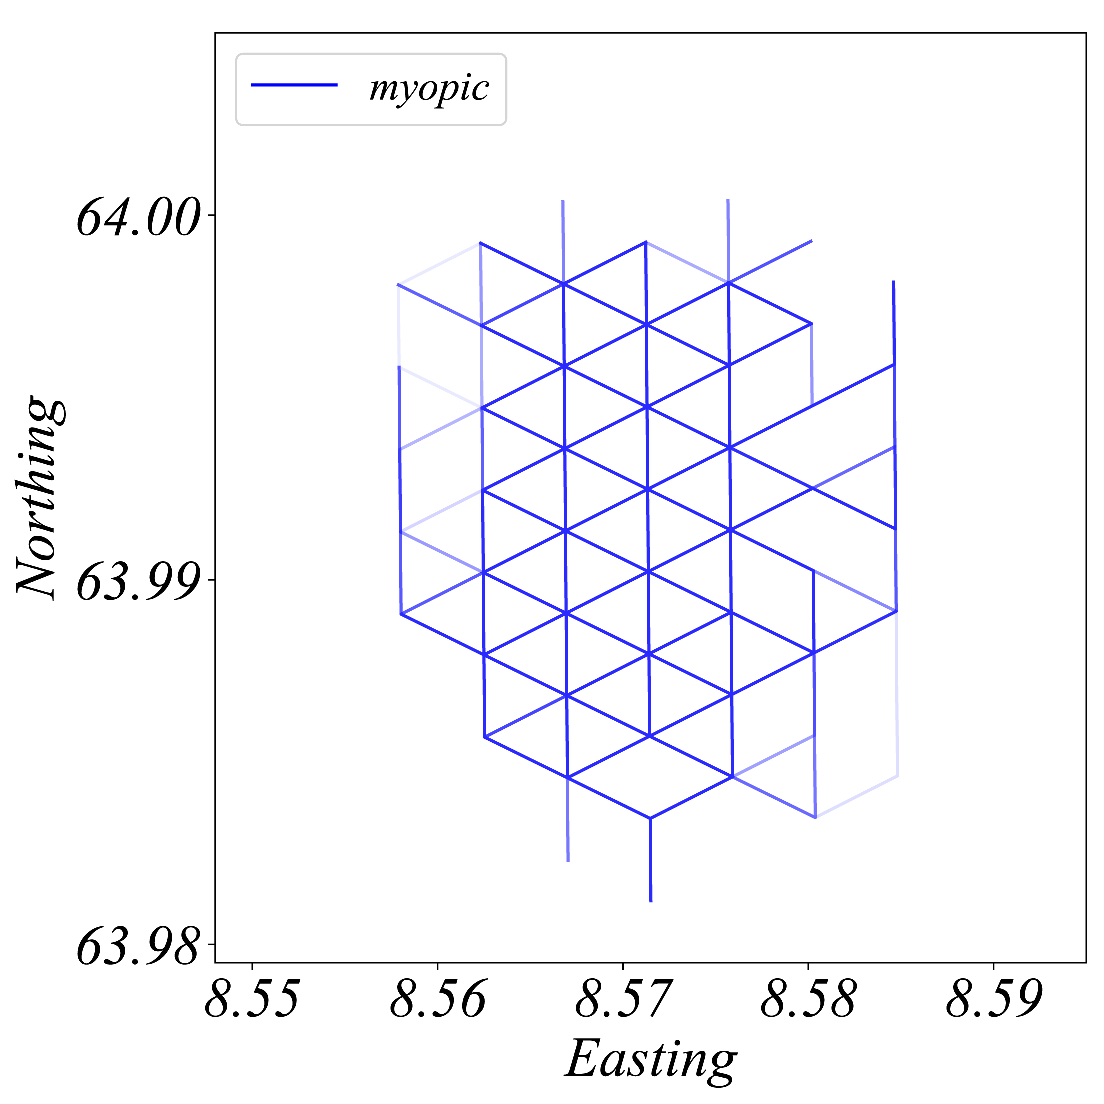
\includegraphics[height = 0.46\textwidth]{Figures/sim/route_myopic.pdf}\label{fig:avg_myopic}}
  \hfill
  \subfigure[Naive]{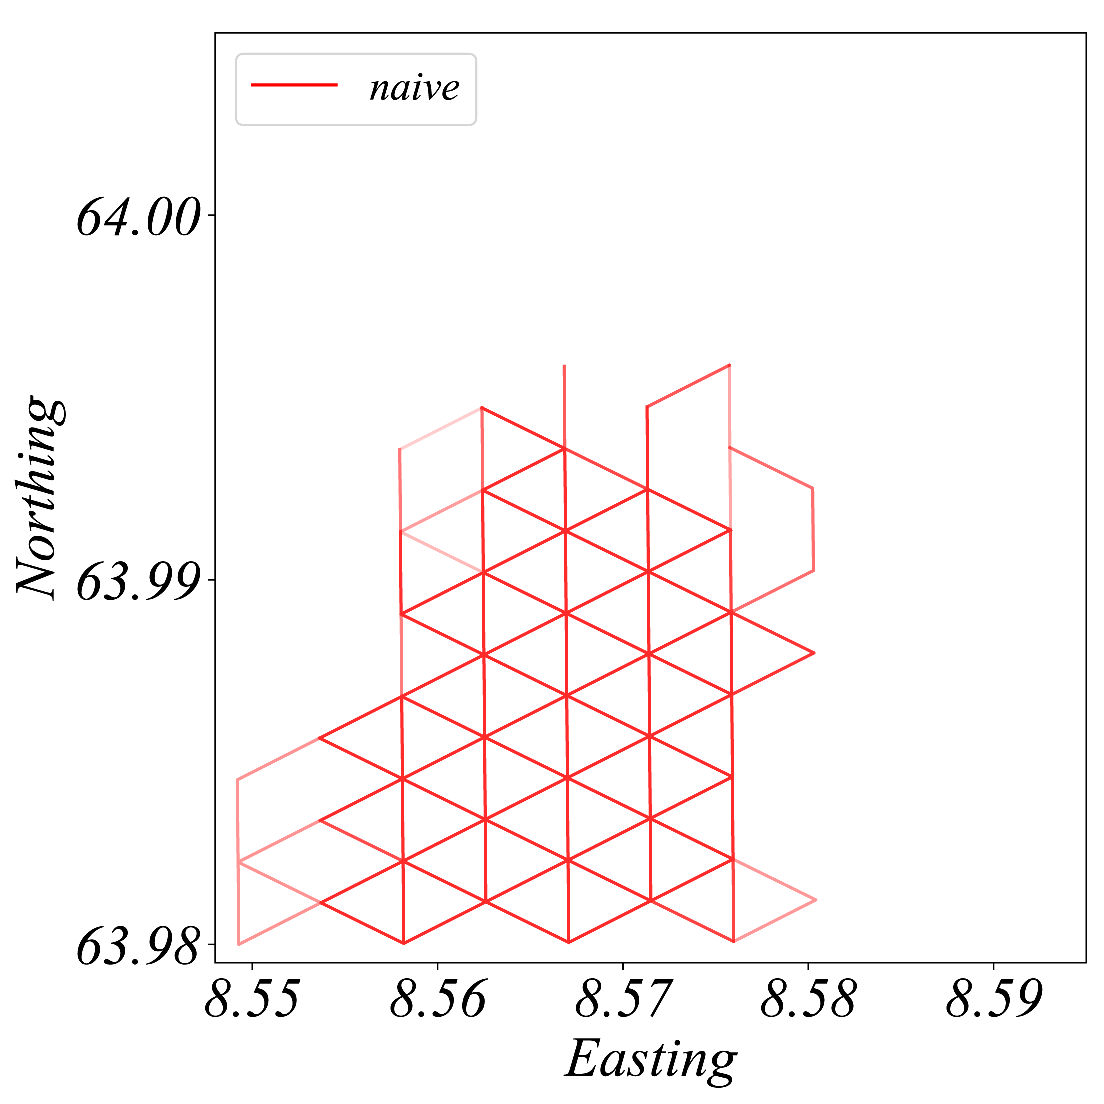
\includegraphics[height = 0.46\textwidth]{Figures/sim/route_naive.pdf}\label{fig:route_naive}}
  \hfill
  \subfigure[Static]{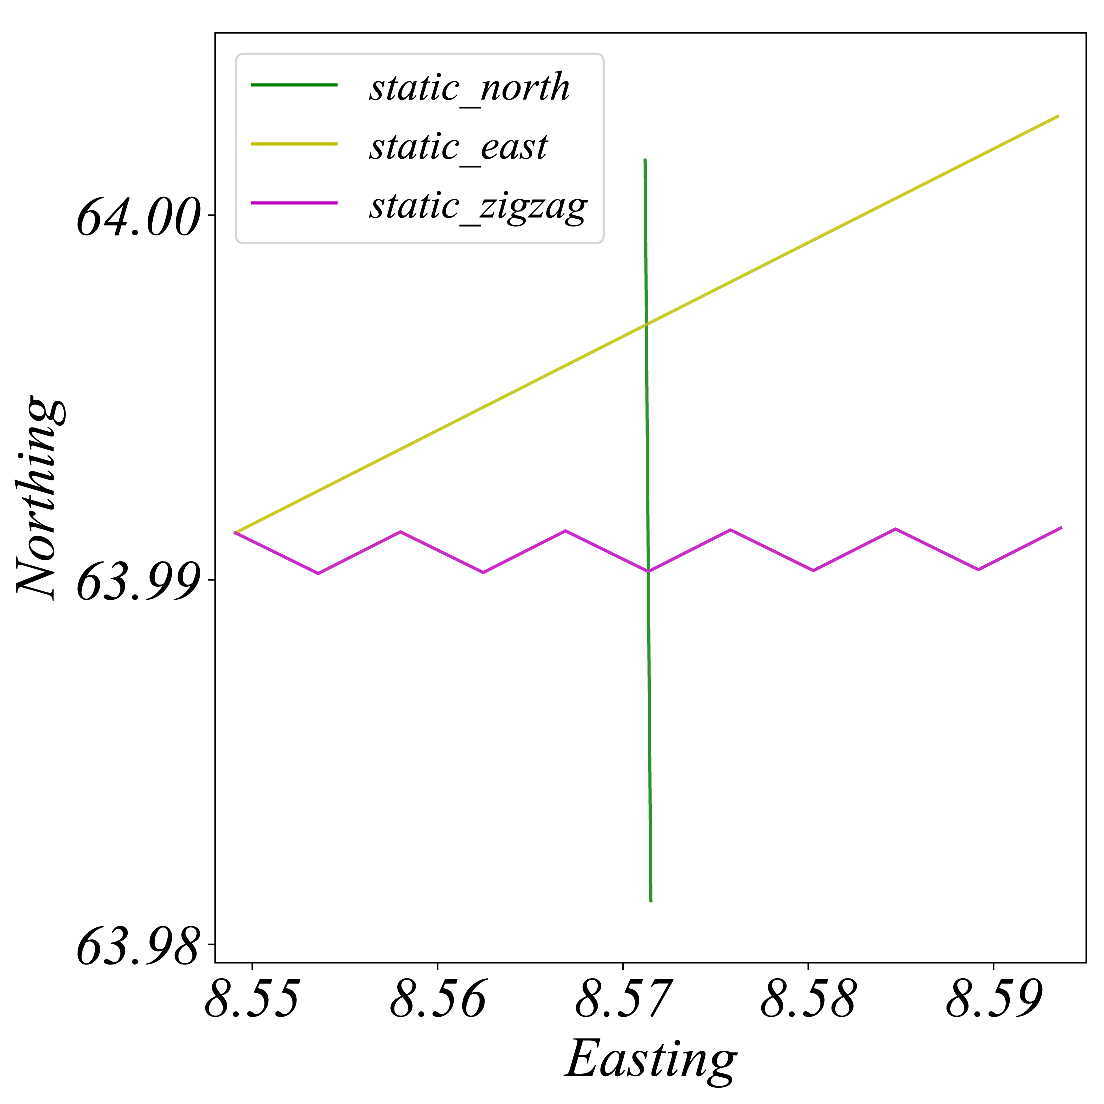
\includegraphics[height = 0.46\textwidth]{Figures/sim/route_static.pdf}\label{fig:route_static}}
  \hfill
  \caption{The overlaid route choices (strategies), superimposed on
    the 100 replicate surveys with 10 sampling choices/stages.}
\label{fig:route_choices}
\end{figure}

Fig. \ref{fig:avg_time} shows the computational effort: the
\textit{naive} strategy is on par with the static designs, while the
\textit{myopic} strategy is slower. The \textit{look-ahead} is even
slower, reaching levels that are nearly impractical for execution on a
vehicle. Some pruning of the graph is performed to improve the
computational speed, such as ruling out repeated visitations and
back-and-forth routes. Some of the intermediate results are also
stored for longer planning horizons. Further pruning of branches or
inclusion of other heuristics could be included to make the strategy
faster. Then again, the inclusion of heuristics is likely a
contributing factor for the \textit{look-ahead} strategy failing to
outperform the \textit{myopic} strategy.

In Fig. \ref{fig:route_choices}, the realized sampling paths for each
of the sequential schemes and static designs are shown. The
\textit{naive} strategy often gets stuck in the southern part of the
domain because it is too focused on the probabilities near $0.5$. The
\textit{myopic} strategy covers a wider domain than the naive or
look-ahead. There are several reasons for this. First, a greedy
approach will tend to put more emphasis on promising locations close to the
agent, which may lead away from the centre. Second, as the agent
evaluates the impact of locations further away (look-ahead) where
assimilated data has less predictive power, the GP model (which
is centered here) will act to restrict paths deviating from the
central zone.

We studied the sensitivity of the results by modifying the input parameters to have different correlations between temperature and salinity, standard deviations, and spatial correlation range.  In all runs,  the \textit{myopic} and \textit{look-ahead} strategies perform the best in terms of IBV, and much better than \textit{naive}. The \textit{look-ahead} strategy seems to be substantially better than the \textit{myopic} only for very small initial standard deviation or very large spatial correlation range. The \textit{static\_north} design continues to be the best static design for IBV, while \textit{static\_zigzag} is the best design for the other predictive performance measures, especially so with large spatial correlation range. We also ran simulation studies with only temperature data, and for realistic correlation levels between temperature and salinity the IBV results are not much worse when only temperature data are available. In addition to the comparison made in Table \ref{tab:sim_rhoab}, the current setting includes spatial correlation and this likely reduces the additional influence of having bivariate data. However, it seems that having temperature data alone does a substantially worse job in terms of explained variance

\begin{comment}
\subsection{Performance Metrics}

The tables below explore the sensitivity of the result to different input correlation values between temperature and salinity measured onboard the AUV, standard deviations, and spatial
correlations (see table rows). We only compare results at the end of
each survey. The expected ES variances are shown in Table
\ref{tab:sim_res_ev}, results of RMSE are in Table
\ref{tab:sim_res_rmse}, and explained variance is in Table
\ref{tab:sim_res_r2}. In all runs, both the \textit{myopic} and
\textit{look-ahead} strategies perform the best in terms of expected
variance in the ES. The \textit{myopic} strategy
performs slightly better than the \textit{look-ahead}. Part of the
reason for this discrepancy can be traced to the act of pruning some
of the paths for the \textit{look-ahead} strategy. The \textit{static\_north} design is clearly
better than the other two static designs, the reason being that the
others do not focus on the areas where the ES is really uncertain
(centre locations are the most uncertain). By measuring temperature
alone, the expected variances in the ES are only slightly higher than
the combined temperature-salinity estimate. This occurs because the
correlation of $0.6$ means that temperature observations provide
information about salinity as well. For the other predictive measures,
\textit{myopic} and \textit{look-ahead} strategies do well, clearly
beating the \textit{naive} strategy. 

\begin{table}[!h]
    \centering
    \scalebox{0.87}{
    \begin{tabular}{lrrrrrr}
    \toprule
    Parameter: $E_{\by}(p[1-p])$ &  naive &  myopic &  look-ahead &  static\_north &  static\_east &  static\_zigzag \\
    \midrule
                    \rowcolor{Gray}
ts. cor. low: 0.2  &  29.65 &   27.08 &       \textbf{26.44} &         32.33 &        40.31 &          36.23 \\
ts. cor. high: 0.8 &  36.18 &   \textbf{28.42} &       30.30 &         32.99 &        37.18 &          36.04 \\
                    \rowcolor{Gray}
std. low: 0.1      &  18.26 &   15.79 &       \textbf{15.35} &         18.89 &        26.65 &          26.10 \\
std. high: 0.5     &  47.01 &   \textbf{41.31} &       43.15 &         47.92 &        52.63 &          49.71 \\
                    \rowcolor{Gray}
cor. low: 0.8      &  44.42 &   \textbf{42.02} &       42.47 &         43.84 &        46.05 &          47.82 \\
cor. high: 0.2     &  29.73 &   21.09 &       \textbf{20.43} &         27.91 &        37.60 &          34.35 \\
                    \rowcolor{Gray}
temp. only         &  38.25 &   29.16 &       \textbf{28.69} &         34.32 &        39.81 &          36.17 \\
basecase           &  35.21 &   \textbf{28.56} &       28.94 &         33.50 &        39.84 &          39.26 \\
    \bottomrule
    \end{tabular}}
  \caption{Simulation results for the final mean IBV (Eq. \eqref{two_partsK}).}
    \label{tab:sim_res_ev}
\end{table}
\vspace{-0.4cm}
\begin{table}[!h]
    \centering
    \scalebox{0.92}{
        \begin{tabular}{lrrrrrr}
        \toprule
        Parameter: RMSE &  naive &  myopic &  look-ahead &  static\_north &  static\_east &  static\_zigzag \\
        \midrule
                \rowcolor{Gray}
ts. cor. low: 0.2  &   0.63 &    \textbf{0.57} &        0.59 &          0.62 &         0.57 &           0.59 \\
ts. cor. high: 0.8 &   0.63 &    \textbf{0.59} &        0.61 &          0.64 &         0.60 &           0.60 \\
                \rowcolor{Gray}
std. low: 0.1      &   0.39 &    0.37 &        0.38 &          0.38 &         0.40 &           \textbf{0.35} \\
std. high: 0.5     &   0.85 &    0.82 &        0.84 &          0.82 &         0.83 &           \textbf{0.81} \\  
                \rowcolor{Gray}
cor. low: 0.8      &   0.68 &    0.66 &        0.67 &          0.68 &         0.66 &           \textbf{0.65} \\
cor. high: 0.2     &   0.58 &    0.54 &        0.55 &          0.58 &         0.54 &           \textbf{0.49} \\
                \rowcolor{Gray}
temp. only         &   0.65 &    0.63 &        0.62 &          0.65 &         \textbf{0.61} &           0.62 \\
basecase           &  0.61 &   \textbf{0.56} &       \textbf{0.56} &         0.60 &        0.57 &          0.57 \\
        \bottomrule
        \end{tabular}}
      \caption{Simulation results for the final mean RMSE ($\frac{1}{B} \sum_{b=1}^{B} \sqrt{(\bmu-\tilde{\bmu})^2}$).}
    \label{tab:sim_res_rmse}
\end{table}
\vspace{-0.4cm}
\begin{table}[!h]
    \centering
    \scalebox{0.95}{
        \begin{tabular}{lrrrrrr}
        \toprule
        Parameter: $\bR^{2}$ &  naive &  myopic &  look-ahead &  static\_north &  static\_east &  static\_zigzag \\
        \midrule
                        \rowcolor{Gray}
ts. cor. low: 0.2  &  27.00 &   33.29 &       32.24 &         26.71 &        30.56 &          \textbf{33.50} \\
ts. cor. high: 0.8 &  23.68 &   \textbf{33.87} &       32.42 &         26.72 &        30.73 &          33.61 \\
                        \rowcolor{Gray}
std. low: 0.1      &  25.38 &   30.80 &       30.29 &         26.09 &        28.75 &          \textbf{31.66} \\
std. high: 0.5     &  26.11 &   34.22 &       32.48 &         26.95 &        31.77 &          \textbf{34.48} \\
                        \rowcolor{Gray}
cor. low: 0.8      &   8.80 &   11.50 &       11.23 &          9.56 &        12.31 &          \textbf{12.58} \\
cor. high: 0.2     &  37.57 &   \textbf{48.68} &       48.11 &         39.61 &        41.98 &          48.04 \\
                        \rowcolor{Gray}
temp. only         &  11.67 &   \textbf{22.82} &       21.98 &         18.16 &        20.77 &          22.78 \\
basecase           &  24.71 &   33.45 &       32.25 &         26.71 &        30.62 &          \textbf{33.54}\\
        \bottomrule
        \end{tabular}}
      \caption{Simulation results for the final mean explained variance $\bR^{2}=100*(1-(\bSigma_{posterior}/\bSigma_{initial}))$).}
    \label{tab:sim_res_r2}
\end{table}

\end{comment}

\section{Case Study - Mapping a River Plume}
\label{sec:case_study}

To demonstrate the applicability of using multivariate EPs and the IBV
to inform oceanographic sampling, we present a case study mapping a
river plume with an AUV. The experiment was performed in Trondheim,
Norway, surveying the Nidelva river (Fig. \ref{fig:nidelven}). The
experiments were conducted in late Spring 2019, when there is still
snow melting in the surrounding mountains so that the river water is
substantially colder than the water in the fjord. The experiment was
focused along the frontal zone that runs more or less parallel to the
eastern shore as noted in Fig. \ref{fig:nidelven}.

\subsection{Model Specification}
\label{sec:exp_modeling}
The statistical model parameters were specified based on a short
preliminary survey where the AUV made an initial transect to determine the trends in environmental conditions and correlation structures. Based on the
initial data, the trend parameters were estimated by linear
regression, where both temperature and salinity are assumed to
increase linearly, going west from the river mouth. Next, the
residuals from the regression analysis were analyzed to study the fit
of the GP model and to specify the covariance parameters.

%\begin{figure}[!h] 
% \centering 
%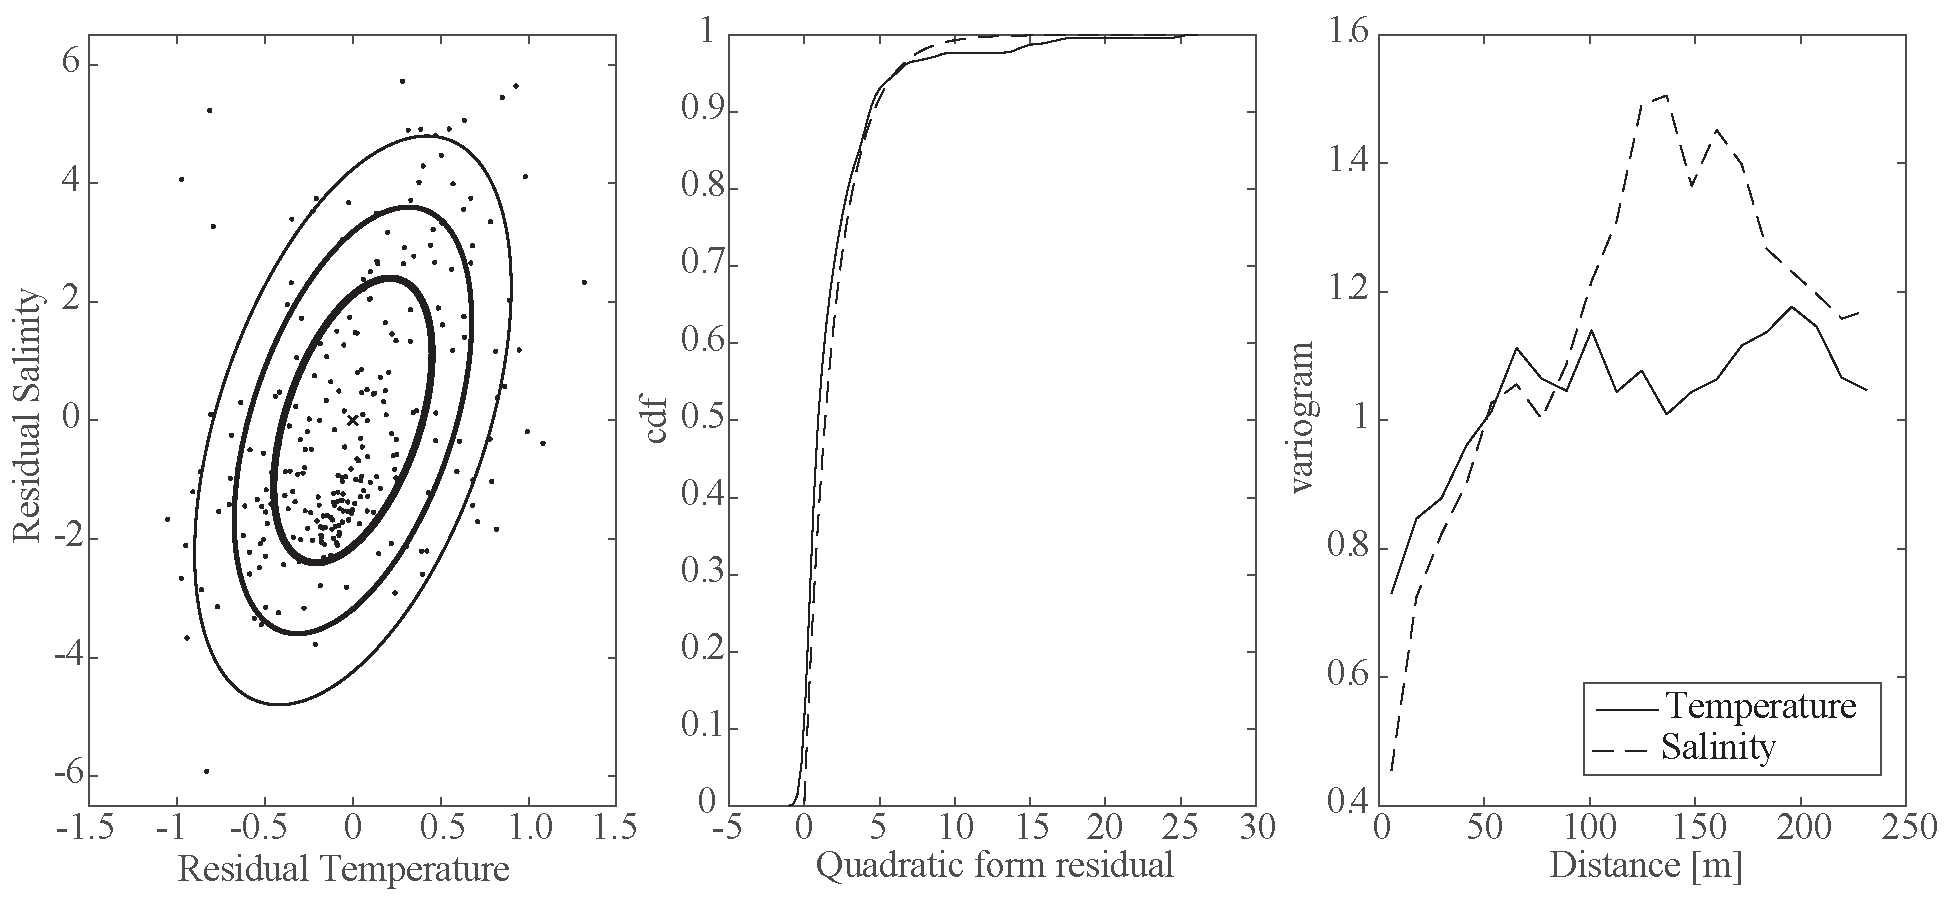
\includegraphics[width=0.98\textwidth]{Figures/field-trials/res_diag.pdf}
%\caption{Data analysis from a preliminary trial experiment using the
%  AUV. Left: Residual plot of temperature and salinity along with
%  Gaussian contours. Middle: Empirical CDF (solid) of the quadratic form of
%  the residuals along with the theoretical CDF (dashed) of the $\chi^2$
%  distribution with two degrees of freedom. Right: Empirical variogram
%  of the salinity and temperature data.} \label{fig:parest}
%\end{figure}

\begin{figure}[!h]
  \centering
  \subfigure[Residual plot.]{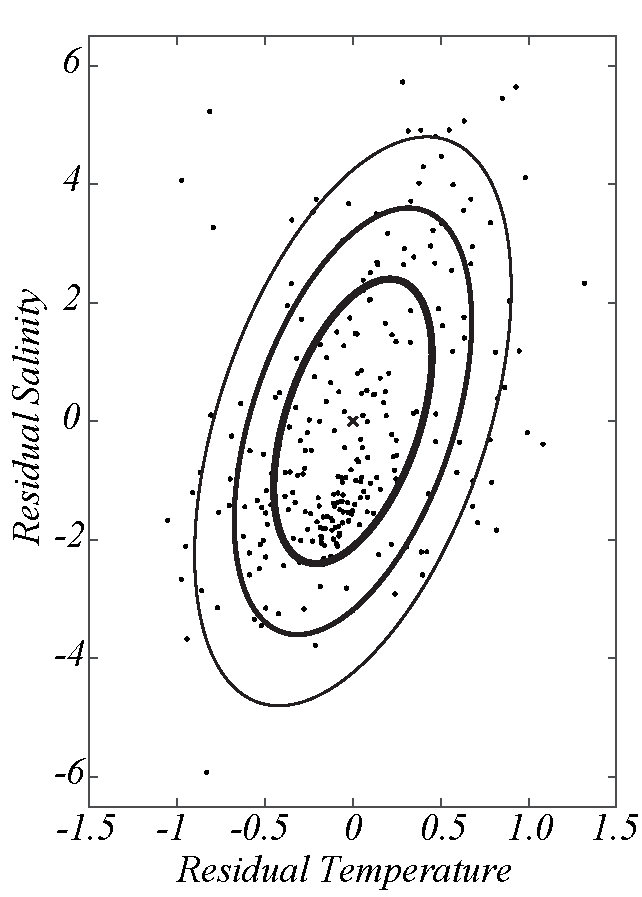
\includegraphics[width = 0.32\textwidth]{Figures/field-trials/res_diag_a.pdf}\label{fig:parest_a}}
  \hfill
  \subfigure[Empirical CDF.]{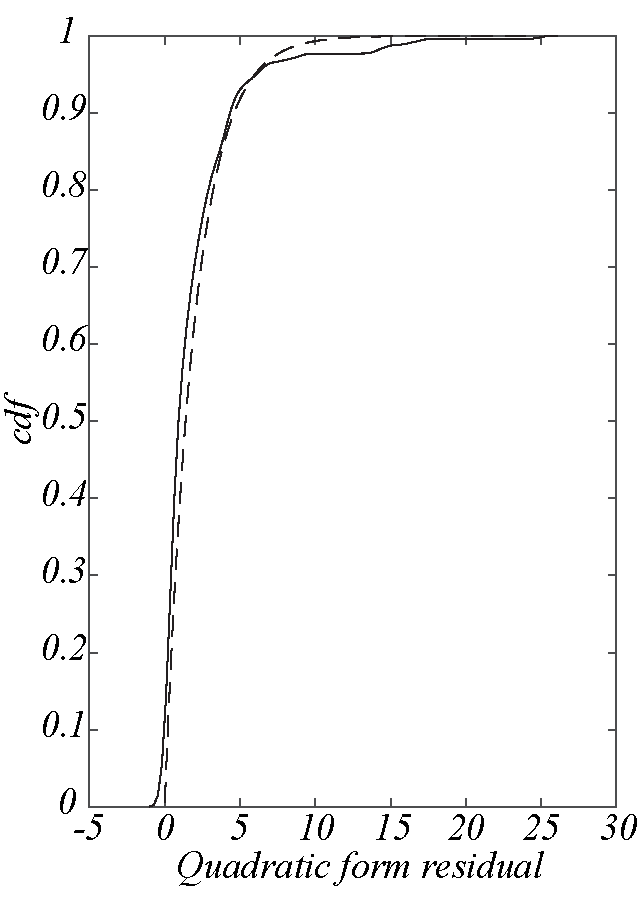
\includegraphics[width = 0.32\textwidth]{Figures/field-trials/res_diag_b.pdf}\label{fig:parest_b}}
  \hfill
  \subfigure[Empirical variogram.]{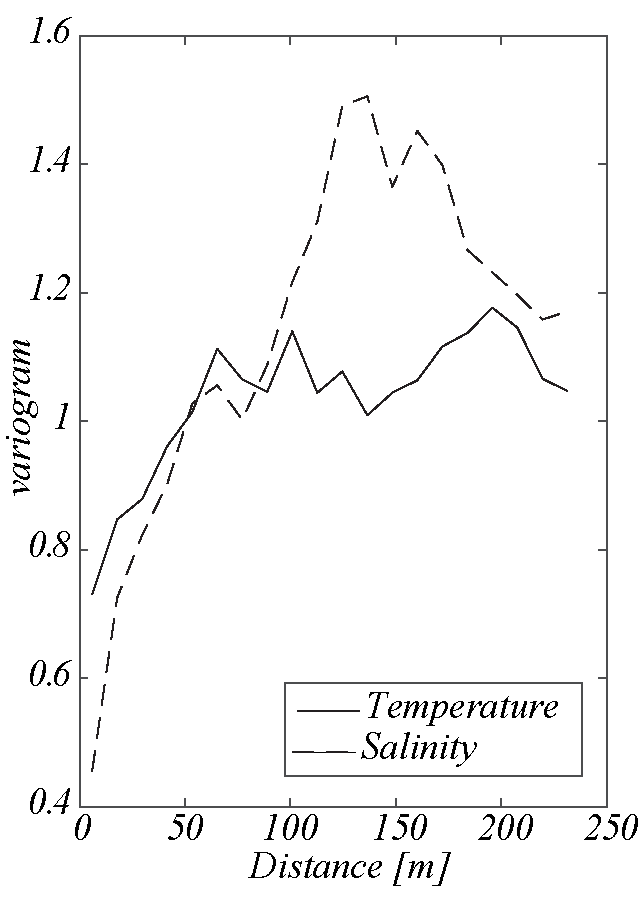
\includegraphics[width = 0.32\textwidth]{Figures/field-trials/res_diag_c.pdf}\label{fig:parest_c}}
  \caption{Data analysis from a preliminary trial experiment using the
    AUV. \ref{fig:parest_a} Residual plot of temperature and salinity
    along with Gaussian contours. \ref{fig:parest_b} Empirical CDF
    (solid) of the quadratic form of the residuals along with the
    theoretical CDF (dashed) of the $\chi^2$ distribution with two
    degrees of freedom. \ref{fig:parest_c} Empirical variogram of the
    salinity and temperature data.}
\label{fig:parest}
\end{figure}

Fig. \ref{fig:parest} summarizes diagnostic plots of this
analysis. Fig. \ref{fig:parest_a} shows a cross-plot of temperature
and salinity residuals after the westerly trends in both salinity and
temperature are subtracted from the data. This scatter-plot of joint
residuals indicates larger variability in salinity than in
temperature, and a positive correlation ($0.5$) between the two
variables. Based on the fitted bivariate Gaussian model (ellipses in
Fig. \ref{fig:parest_a}), we can compute the modeled quadratic form of
the residuals, and if the model is adequate they should be
approximately $\chi^2_2$ distributed. Fig. \ref{fig:parest_b} shows
the empirical cumulative distribution function (CDF) of these
quadratic forms (solid) together with the theoretical CDF of the
$\chi^2_2$ distribution. The modeled and theoretical curves are very
similar, which indicates that the Gaussian model fits reasonably
well. Even though there appears to be some clustering in both
Fig. \ref{fig:parest_a} and \ref{fig:parest_b}, the bivariate
diagnostic plots look reasonable and justify a Gaussian
model. Fig. \ref{fig:parest_c} shows the empirical variogram of the
scaled residuals for temperature and salinity. The decay is similar
for the two, and seems to be negligible after about $150$ m.


Based on the analysis in Fig. \ref{fig:parest}, the resulting
parameters are given in Table \ref{tab:experiment_param}. The
regression parameters shown here are scaled to represent the east and
west boundaries of the domain as seen in the preliminary transect
data, and the thresholds are intermediate values. These parameter
values were then used in field trials where we explored the
algorithm's ability to characterize the river plume front separating
the river and fjord water masses, providing a spatial map of this
boundary.

%Mapping the spatial extent of a frontal zones is an important problem for studying many bio-physical interactions in the ocean. The frontal zone is determined by the boundary where plumes of sediments, nutrients, and possibly pollutants spreading from the river outlet meet and interact with adjacent coastal water. Due to the lower density the plumes spread on the surface, creating a front with an sharp gradient in both temperature and salinity. 

\begin{table}[!h]
\centering
\begin{tabular}{lrr}
\toprule
Parameter & Value & Source\\
\midrule
\rowcolor{Gray}
Cross correlation temp. and sal. & 0.5 & AUV observations\\
Temp. variance &  0.20 & AUV observations (variogram)\\
\rowcolor{Gray}
Sal. variance &  5.76 & AUV observations (variogram)\\
Corr. range  & 0.15 km & AUV observations (variogram)\\
\rowcolor{Gray}
River temp. $T_{river}$ & $10.0\,^{\circ}\mathrm{C}$ & AUV observations\\
Ocean temp. $T_{ocean}$ & $11.0\,^{\circ}\mathrm{C}$ & AUV observations\\
\rowcolor{Gray}
River sal. $S_{river}$ & $14.0$ g/kg & AUV observations\\
Ocean sal. $S_{ocean}$ & $22.0$ g/kg & AUV observations\\
\rowcolor{Gray}
Threshold temp. & $10.5\,^{\circ}\mathrm{C}$ & $(T_{ocean}-T_{river})/2+T_{river}$\\
Threshold sal. & $18.0$ g/kg & $(S_{ocean}-S_{river})/2+S_{river}$\\
\rowcolor{Gray}
\bottomrule
\end{tabular}
\caption{Model and threshold parameters from an initial AUV
  survey. Observations were taken across the front while crossing from
  fresh, cold river water to saline and warmer ocean waters.}
\label{tab:experiment_param}
\end{table}


\subsection{Experimental Setup}

The sampling locations were distributed over an equilateral grid, as
shown in the grey-colored lattice in Fig. \ref{fig:map}. The robotic
platform consisted of a Light AUV \citep{sousa2012lauv}
(Fig. \ref{fig:lauv}) equipped with a 16 Hz Seabird Fastcat-49
conductivity, temperature, and depth (CTD) sensor providing
temperature and salinity
measurements. %The accuracy of the CTD instrument is $\pm 0.0003$ S/m (conductivity) and $\pm0.002\,^{\circ}\mathrm{C}$ (temperature).
The sampling agent was built on top of the autonomous agent framework
Teleo-Reactive EXecutive (\textit{T-REX})
\citep{py10,Rajan12,Rajan12b}, running an instance of the
\textit{myopic} strategy from Section \ref{sec:myopic} to
control the AUV and decide between sampling locations.

\begin{figure}[!h] 
\centering 

\includegraphics[width=0.98\textwidth]{Figures/harald.jpg}
\caption{The commercially available Light Autonomous Underwater
  Vehicle (LAUV) platform for upper water-column exploration used in
  our experiments.}
\label{fig:lauv}
\end{figure} 

The sampling strategy was designed around the concept of visiting
waypoints sequentially. Arriving at a desired waypoint with new
measurements and an updated model, the AUV triggers the myopic
strategy to evaluate the different design criteria (see
Eq. \eqref{critSEQ}). The waypoint-and-path combination that is
expected to reduce the IBV the most is selected, and upon arrival this
procedure is then repeated. At each stage, it takes the AUV about 30
seconds to evaluate the expected IBV for all the possible
waypoint-and-path alternatives.

The AUV was set to start in the south-center part of the waypoint
graph, with the previously outlined GP model of the environment (Section \ref{sec:exp_modeling}). A
survey was set to take approximately 40 minutes, visiting 15 waypoints
on the grid, with the AUV running near the surface to capture the
plume. On its path from one waypoint to the next, the AUV gathered
data regularly, and the GP model assimilated temperature and salinity
data with an update frequency of 30 seconds, giving about three updates
per stage.

\begin{figure*}[!h]
\centering
\subfigure[Survey map]{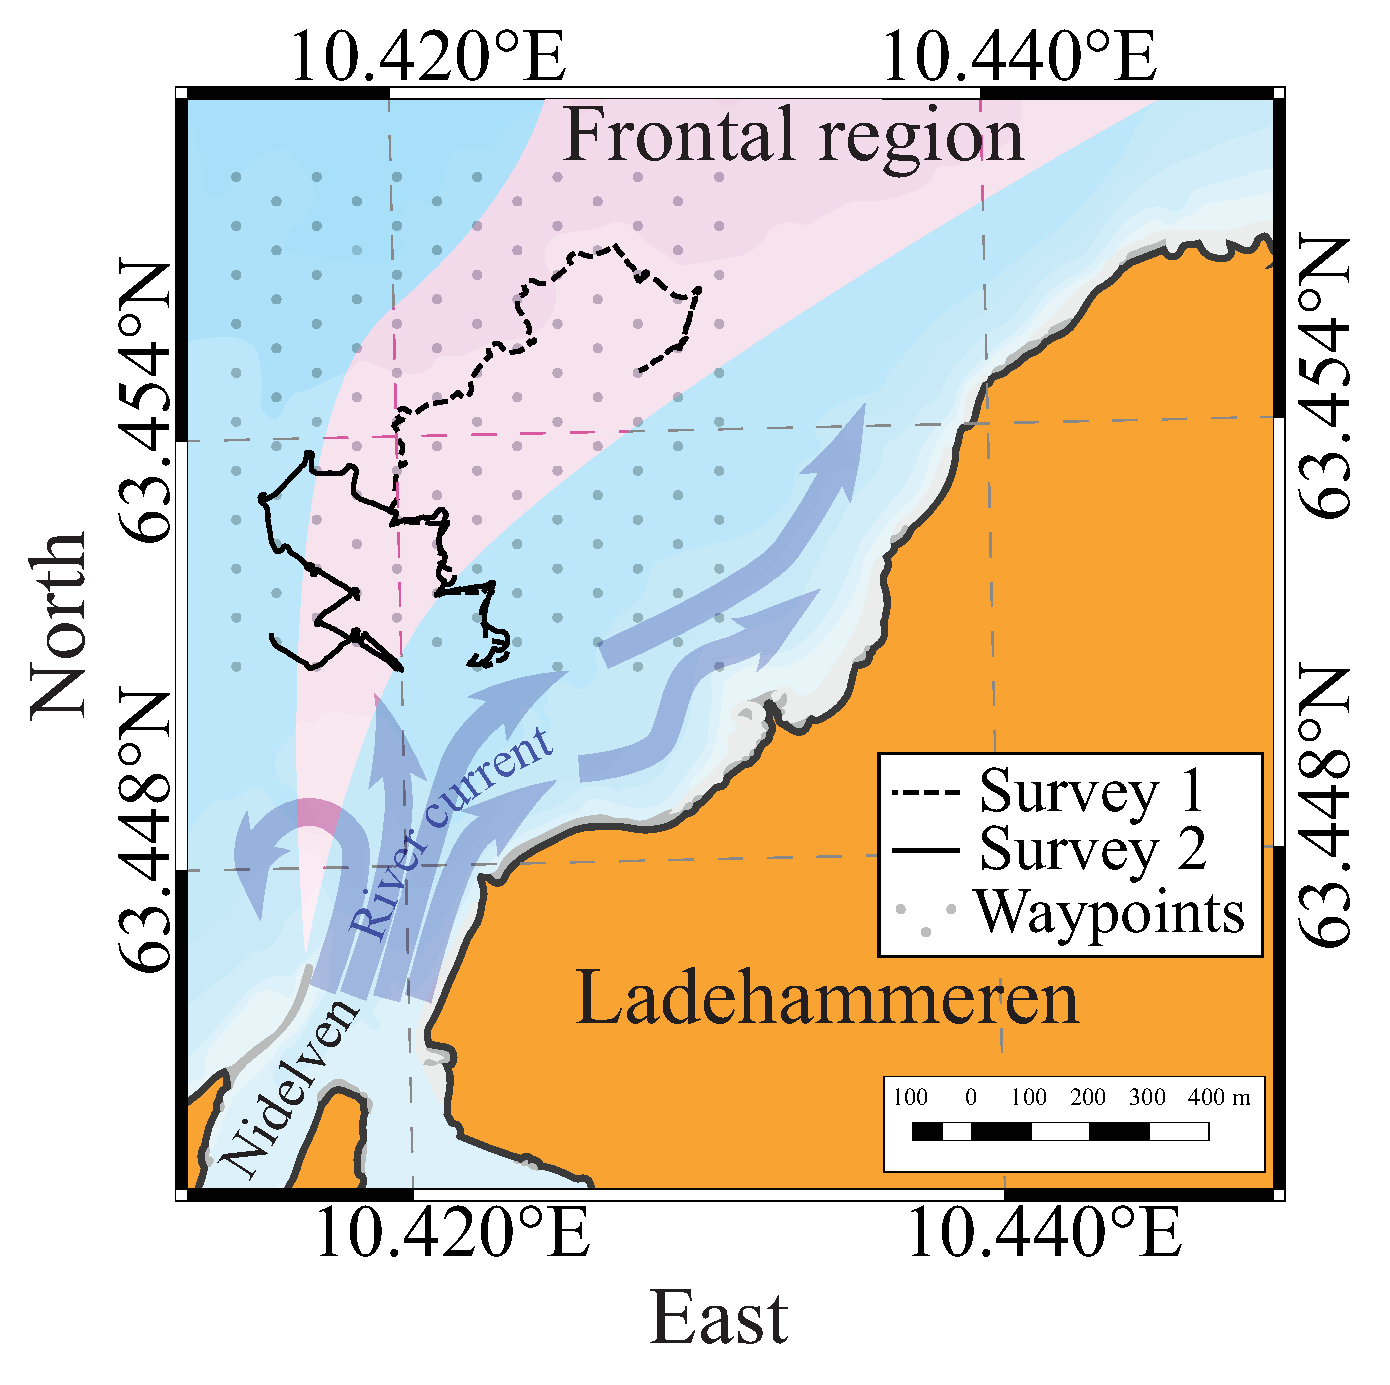
\includegraphics[height=0.41\textwidth]{Figures/field-trials/alt_map.eps}\label{fig:map}}
\hspace{0.3cm}
\subfigure[Temperature tracks]{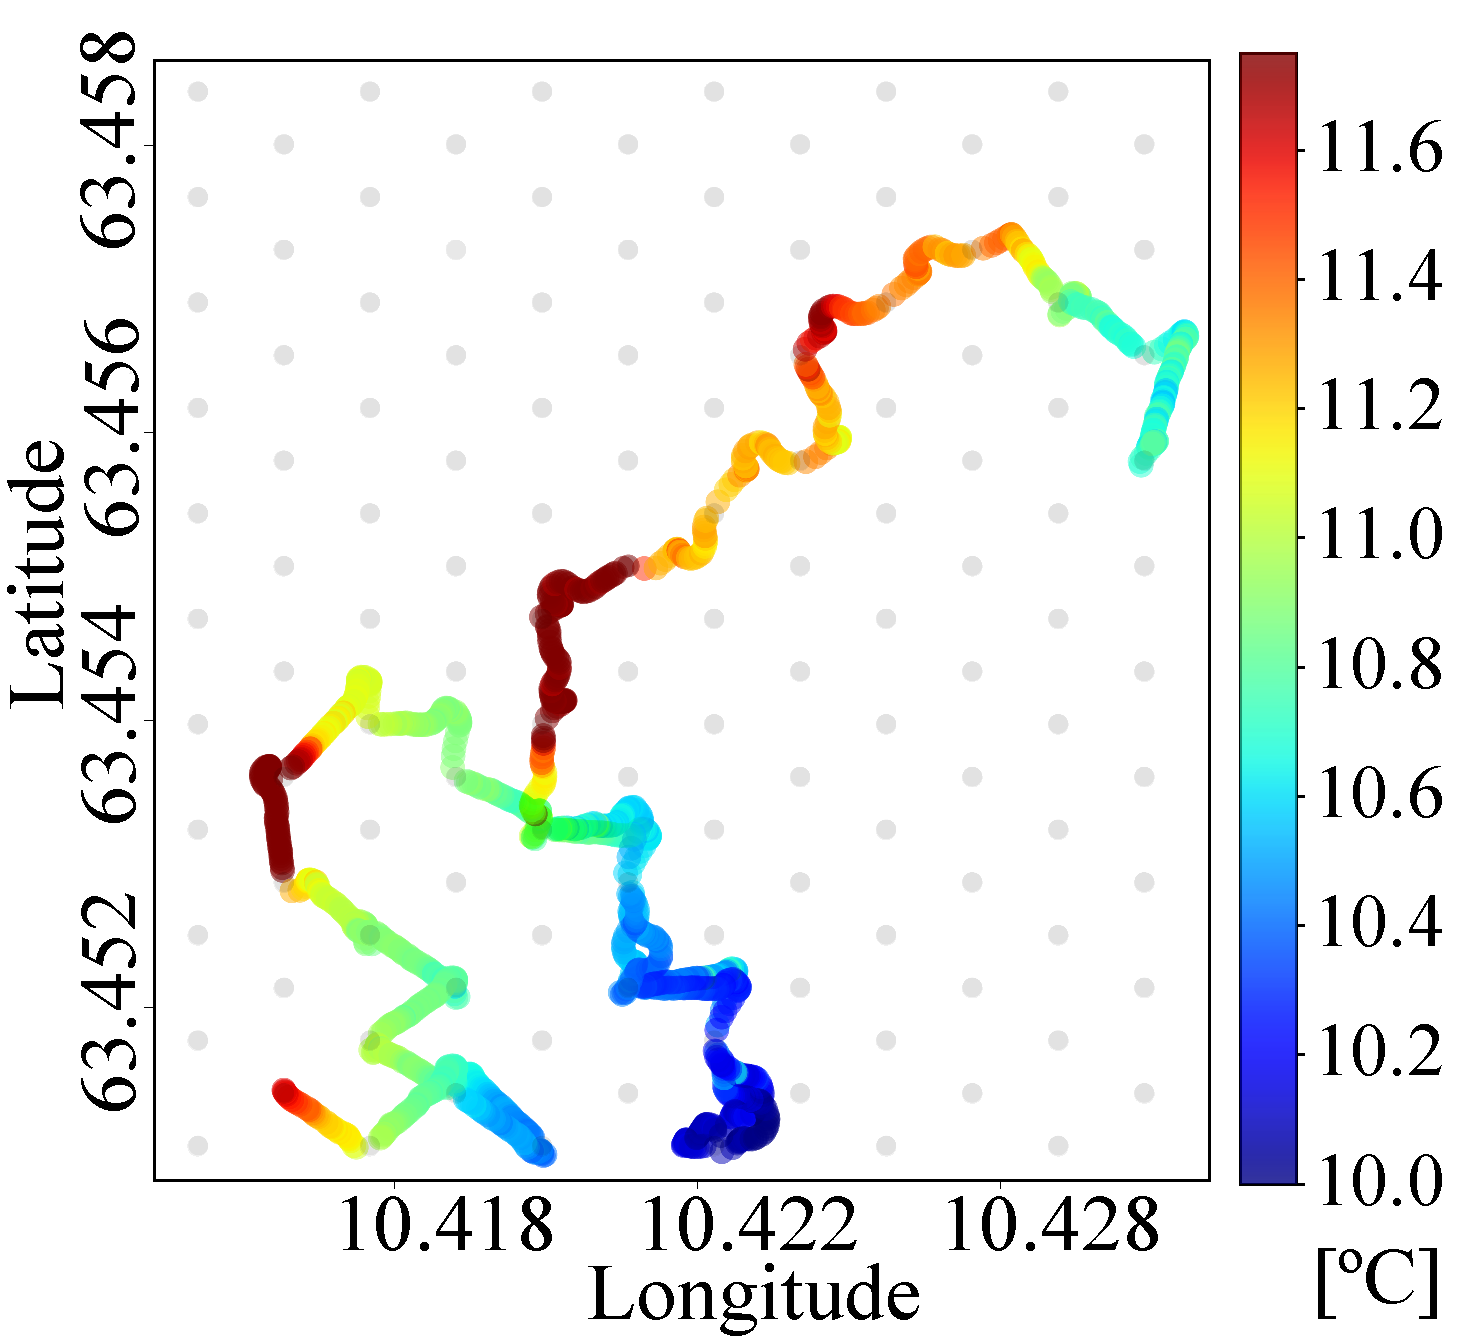
\includegraphics[height=0.41\textwidth]{Figures/field-trials/auv.pdf}\label{fig:res_both}}

\subfigure[Survey 1]{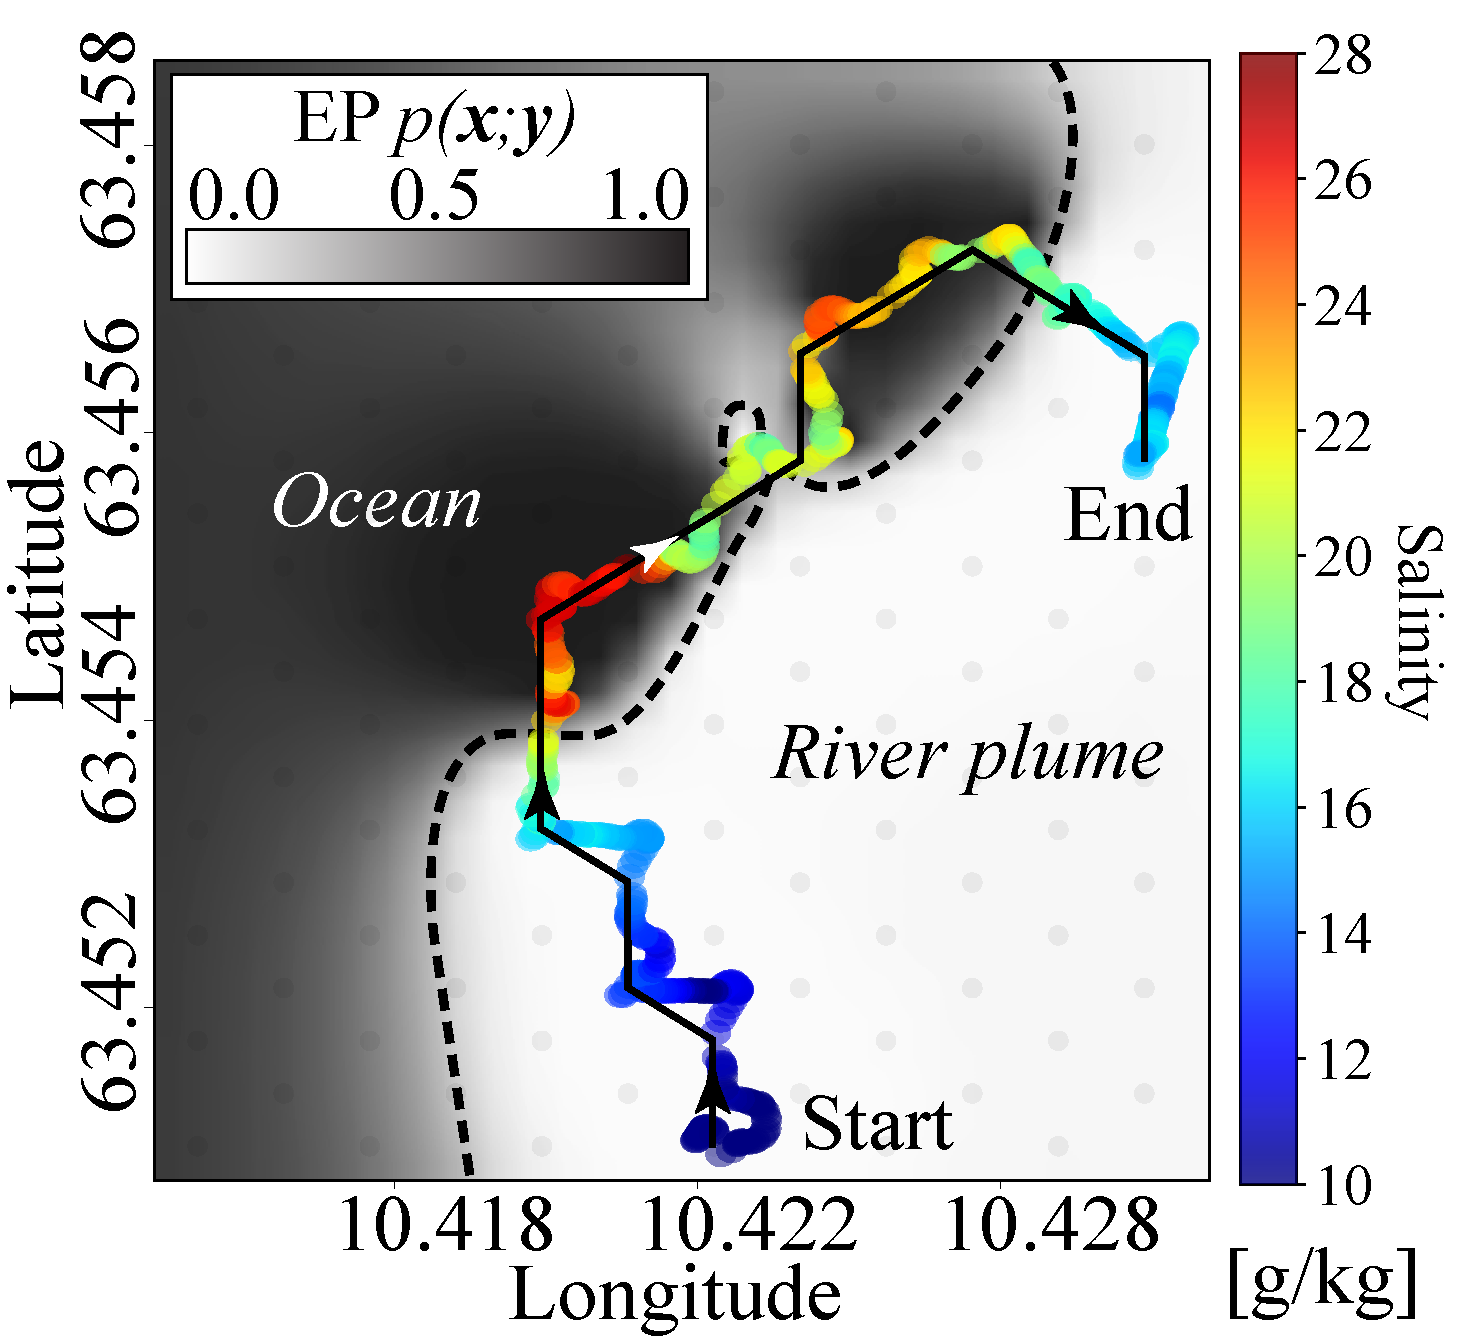
\includegraphics[height=0.40\textwidth]{Figures/field-trials/auv1_es_sal_ep.pdf}\label{fig:res1}}
\hspace{0.2cm}
\subfigure[Survey 2]{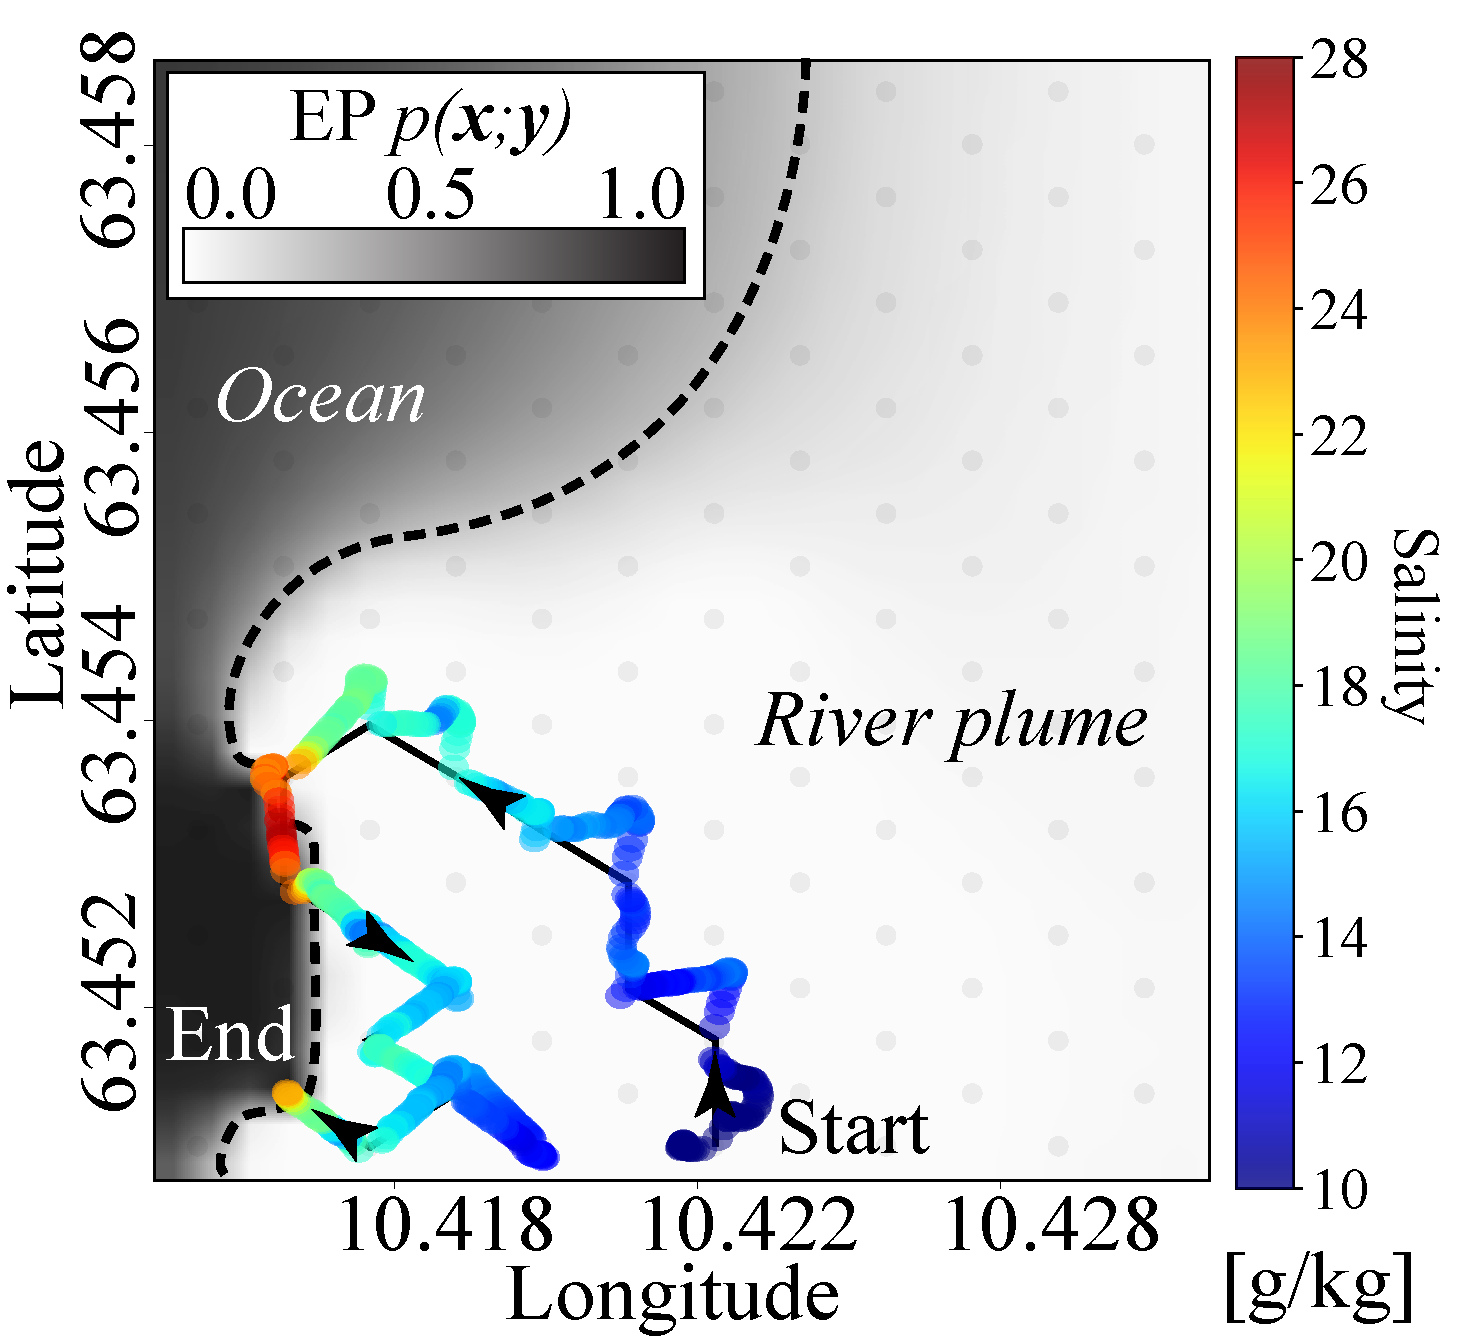
\includegraphics[height=0.40\textwidth]{Figures/field-trials/auv4_es_sal_ep.pdf}\label{fig:res2}}

%\subfigure[ES for Survey 1]{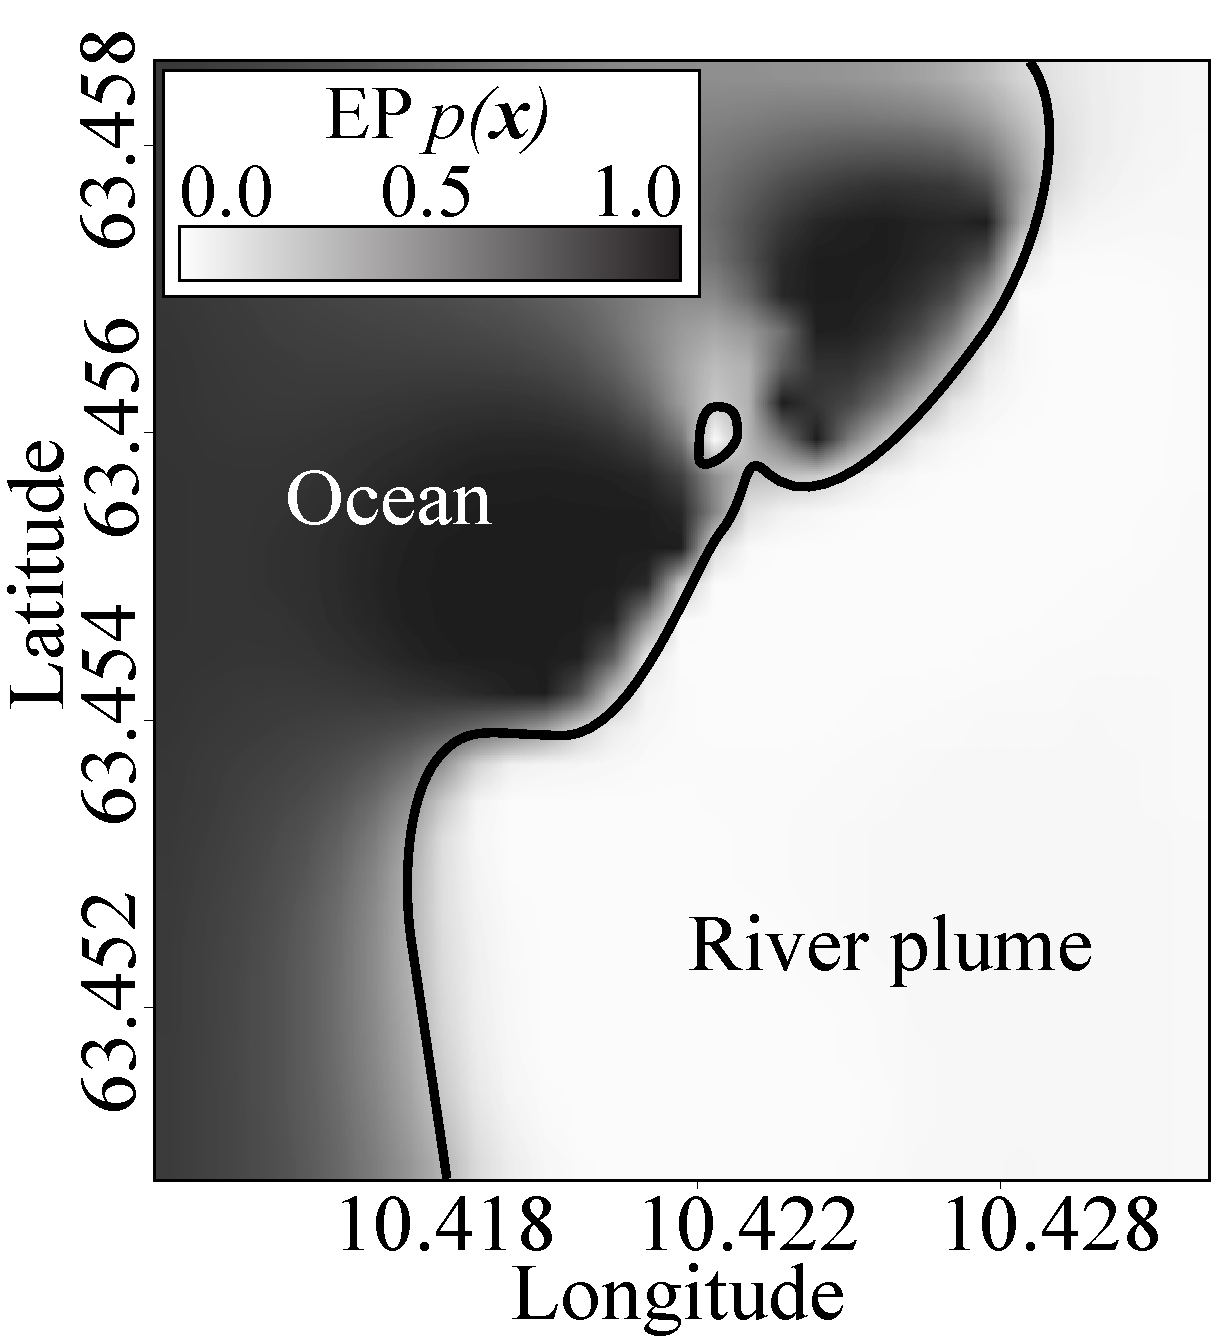
\includegraphics[height=0.41\textwidth]{Figures/field-trials/ep_1.pdf}\label{fig:res3}}\hspace{0.4cm}
%\subfigure[ES for Survey 2]{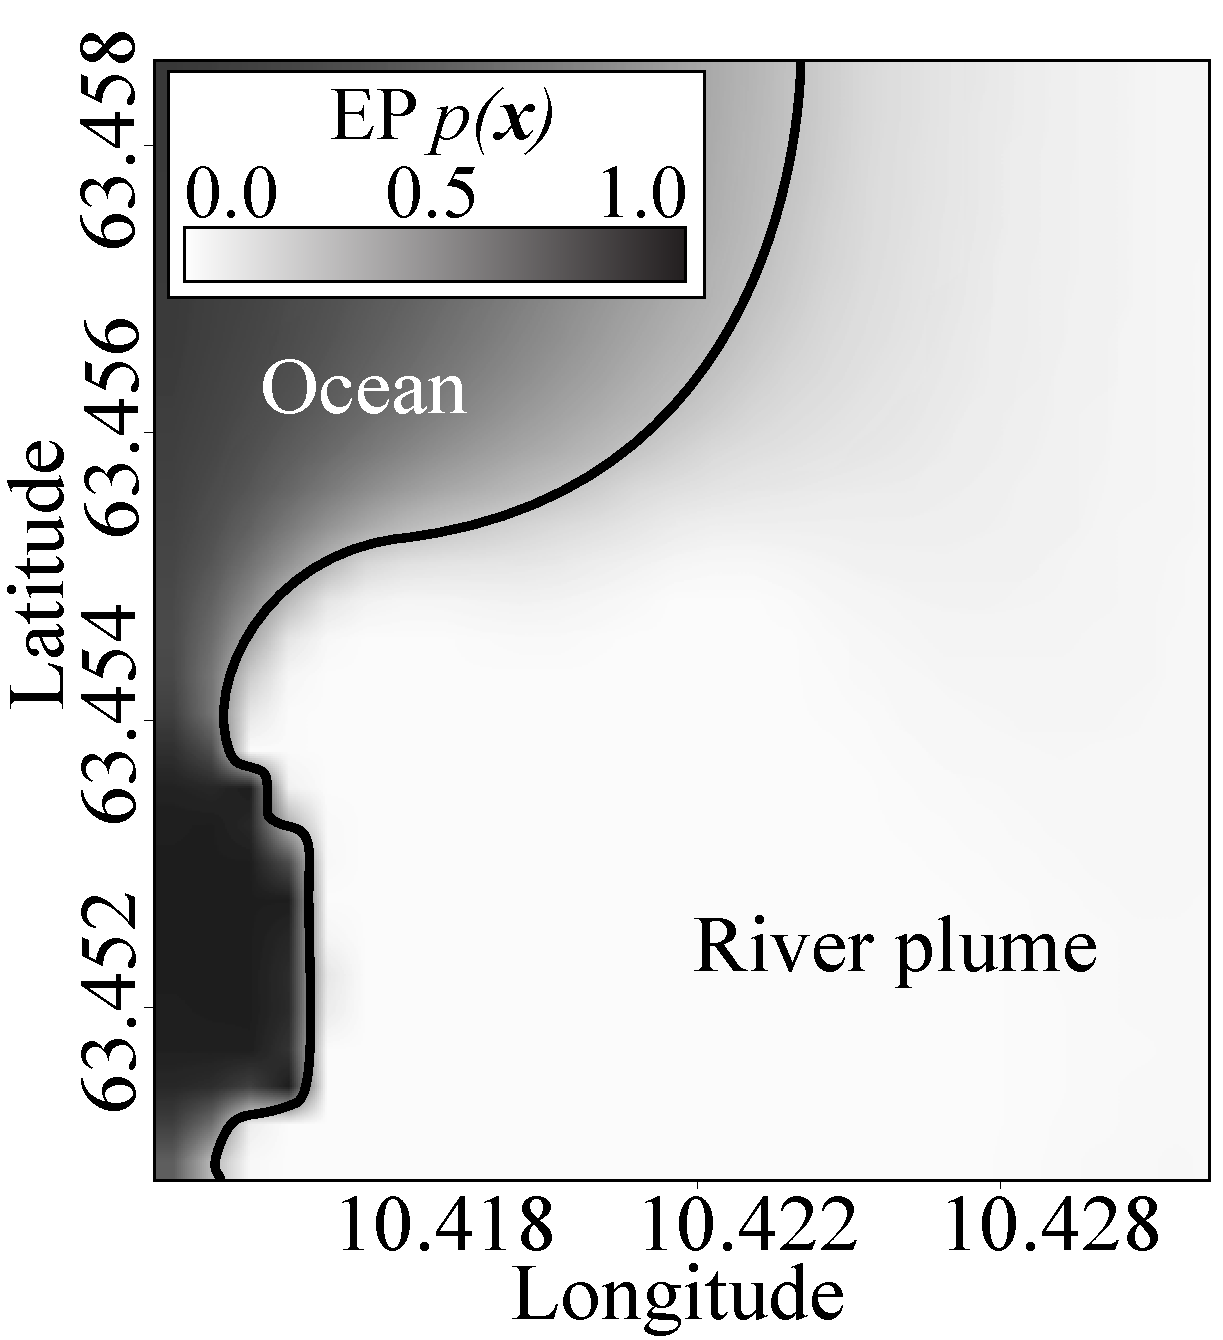
\includegraphics[height=0.41\textwidth]{Figures/field-trials/ep_4.pdf}\label{fig:res4}}
\caption{Results from mapping the Nidelva river. \ref{fig:map} Show an
  overview of the survey area overlaid with the AUV path in black and
  dashed line. Note the shaded region indicating the usual frontal
  region. \ref{fig:res_both} Presents the collected temperature data
  as colored trails. Note waypoint 5 (WP5) which indicate where the
  two surveys deviate. \ref{fig:res1} and \ref{fig:res2} Shows the
  collected salinity data (as a colored trail) overlaid on the final
  EP, which indicate the AUVs statistical impression of the front. For
  both missions the temperature and salinity data correspond with the
  EP front indication.}
\label{fig:results}
\end{figure*}

\subsection{Results}

Two missions, Surveys 1 and 2, were run successively from 11:00 AM to
01:00 PM, with a short break in between. The resulting path of the
selected waypoints are shown in the map in Fig. \ref{fig:map}, both
within the expected frontal region (shaded pink). The recorded
temperatures are shown as colored trails in Fig. \ref{fig:res_both},
clearly indicating the temperature difference between fjord and river
waters. The salinity data are then shown separately, overlaid with the
estimated EP for each survey in Fig. \ref{fig:res1} and
\ref{fig:res2}.

Both surveys successfully estimated and navigated the separation zone,
crossing the frontal boundary multiple times. As conditions changed
slightly between the two deployments, the resulting path (after
waypoint 5) is shown to deviate. Survey 1 continued northwards,
tracking the north-eastern part of the front, while Survey 2 turned
west, mapping the south-western part.

The final predictions of the front location, represented by conditional EPs in
Fig. \ref{fig:res1} and \ref{fig:res2} as dashed lines, correspond
with one another. In both surveys they yield a picture of the front being a bit to the west in the southern parts of the domain and gradually bending off toward the north east. The amount of exploration done by Survey 1
is greater than Survey 2. In Survey 1, the AUV obtained more detail by
going north from waypoint 5, while Survey 2, coming close to the survey area borders
in the south-western corner, obtained a poorer understanding of the
northern parts. A look-ahead strategy might identify and
discourage such choices.

%\begin{figure}[!h] 
% \centering 
%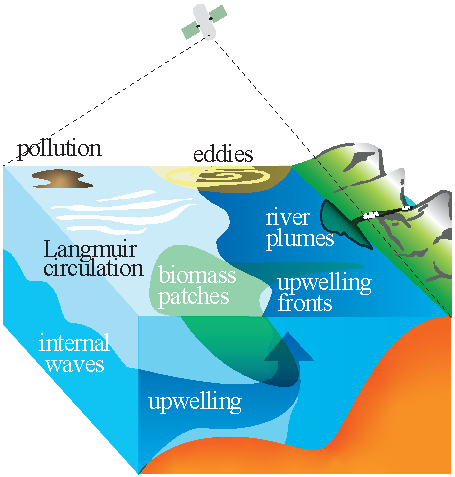
\includegraphics[width=0.48\textwidth]{Figures/envir_ocean.pdf}
%\caption{Ocean observation is moving away from %single-ship sampling
%towards more collaborative networked operations in %order to resolve
%the numerous processes and their interaction.} %\label{fig:envir}
%\end{figure}
\newpage
\section{Closing remarks}\label{sec:concl_disc}

This work builds on a multidisciplinary effort combining statistical
modeling with robotic surveying techniques for oceanographic
applications. We show how observation practices can gain efficiency
and accuracy from the development of statistical techniques to achieve
more effective spatial monitoring. We further demonstrate the
opportunities available for real-time multivariable spatial
data-gathering and analysis onboard autonomous sensing platforms,
which statisticians can exploit to create general-purpose toolkits for
similar applications.

In particular, we derive and show results for characterizing phenomena
connected to the properties of water masses. The characterization is
based on joint ESs, whereby we derive new results for the expected IBV
reduction achieved by the spatial sampling design. This result is
first calculated in closed form for the situation with a static
design, and then extended to the adaptive situation. The sequential
derivations provide new insights into efficient applications of
adaptive sampling, as demonstrated in our application of these models
with an autonomous vehicle in Trondheim fjord.

The study did not consider any temporal effects, which would be
relevant on a larger time scale. We consider the extension to
spatio-temporal modeling as future work, and envision that
advection-diffusion equations could be useful in this kind of modeling
\citep{sigrist2015stochastic}. For more complex oceanographic
phenomena, the methods will need to be extended to non-Gaussian
phenomena, possibly feature-based mixtures of GPs which could still be
run onboard and augmented by dynamical models.

The spatial-statistical design criterion, building on ESs, is relevant
in our setting with different water mass properties; this could also
be useful in other oceanographic settings, such as algal-blooms or
open water fronts. Of course, other criteria are also relevant for
decision-making. For instance, managers and regulators must make
difficult decisions related to fish farming, other marine resources
operations, or environmental projects. Value of information analysis
(VOI) \citep{Eidsvik:15} could be used in a similar vein as the IBV in
the current paper, as both analytic methods explore when, where and
which information is likely to result in improved decision-making.

While more effort could be spent on approximating the look-ahead stages
in the adaptive designs, it is perhaps more interesting to explore the
additional flexibility that can be gained by having two or more AUVs
co-temporally exploring a spatial or spatio-temporal domain together
\citep{ferreira2019advancing}. Such an approach would enable
concurrent sampling in different parts of the space, or opportunities
to move in parallel to best capture the excursion set.

\section*{Acknowledgements}

TOF and KR acknowledge support from the Centre for Autonomous Marine
Operations and Systems
(AMOS)\footnote{\url{https://www.ntnu.edu/amos}}, Center of
Excellence, project number 223254, and the Applied Underwater Robotics
Labortatory (AURLab). JE acknowledges support from Norwegian research
council project 294404. DG acknowledges support from the Swiss
National Science Foundation, project number 178858.

%\begin{supplement}
%\sname{Supplement A}\label{suppA}
%\stitle{Title of the Supplement A}
%\slink[url]{http://www.e-publications.org/ims/support/dowload/imsart-ims.zip}
%\sdescription{Dum esset rex in
%accubitu suo, nardus mea dedit odorem suavitatis. Quoniam confortavit
%seras portarum tuarum, benedixit filiis tuis in te. Qui posuit fines tuos}
%\end{supplement}

% == Adding references
\footnotesize
\bibliographystyle{imsart-nameyear}
\bibliography{ref}

% AOS,AOAS: If there are supplements please fill:
%\begin{supplement}[id=suppA]
%  \sname{Supplement A}
%  \stitle{Title}
%  \slink[doi]{10.1214/00-AOASXXXXSUPP}
%  \sdatatype{.pdf}" 
%  \sdescription{Some text}
%\end{supplement}

\end{document}
